\documentclass[a4papper]{article}
\usepackage[left=0.5cm,right=0.5cm,top=2cm,bottom=0.5cm,bindingoffset=0cm]{geometry}
\usepackage{header-linear-algebra}

\title{\Huge Линейная алгебра, Экзамен}

\author{
    Написано простым \href{https://t.me/Borislav_Timoshin}{BIT}-ом на основе лекций Гордеевой Н.М., \\ 
    учебника Канатникова А.Н., Крищенко А.П., \\
    методичек Власова П.А., Соболева С.К., \\
    записей одногруппников и старшекурсников,\\ некоторых методичек Мехмата МГУ и, конечно, \\ с помощью одного загадочного, вдохновляющего на \\ изучение математики путешественника по млечному пути, \\
    приносящего умные мысли в процессе \\
    нашего общего мозгового штурма. \\
    \href{https://github.com/BorislavTimoshin/Linear-Algebra-BMSTU-BS1-Exam-}{GitHub}.
}

\date{} % Очищаем стандартную дату

\begin{document}
    \pagestyle{fancy}
    \fancyhead[L]{\thepage}
    \fancyhead[R]{\hyperlink{toc}{\large Содержание}}

    \maketitle

    \epigraph{
        ``Верю, что проникну в пространство, невидимое доселе, и буду творить в нем чудеса!!''.
    }{\rightline{{\rm --- BIT}}}


    \vfill % Добавляем вертикальное заполнение, чтобы сдвинуть вниз

    \begin{center}
        \Large МГТУ им. Н.Э. Баумана, кафедра ФН1. \\
        \emph{2024 — 2025}
    \end{center}

    \newpage
        
    \tableofcontents

    \Hide

\part{Модуль 1.}

\section{
    Комплексные числа. Арифметические действия над комплексными числами. Возведение в степень и извлечение корня. Комплексная плоскость, модуль, аргумент. Формула Эйлера. Формула Муавра.
}

% Комплексные числа
\subsection{
    Комплексные числа.
}

\begin{definition}
    \textbf{\textit{Комплексным числом $z$}} называется пара $(x, y)$ действительных чисел $x, y \in \RR$, для которой определены понятие равенства и операции сложения и умножения следующим образом:
    
    \begin{enumerate}[nosep]
        \item $z_1 = z_2 \iff x_1 = x_2$ и $y_1 = y_2$.
        \item $z_1 + z_2 = (x_1 + x_2, \thinspace y_1 + y_2)$.
        \item $z_1 \cdot z_2 = (x_1x_2 - y_1y_2, \thinspace \thinspace x_1y_2 + x_2y_1)$
    \end{enumerate}
\end{definition}

\begin{designation}
    $\CC$.
\end{designation}

\begin{definition}
    \textbf{\textit{Мнимой единицей}} называется число $i = (0, 1)$, причем ее квадратом, является пара $(-1, 0)$.
\end{definition}

\begin{definition}
    Комплексное число $\overline{z}$ называется \textbf{\textit{сопряженным}} к $z$, если $\overline{z} = x - iy$, $z = x + iy$.
\end{definition}

\textbf{Свойства комплексного сопряжения.}

\begin{enumerate}[label={\arabic*°.}]
    \item $\overline{z + w} = \overline{z} + \overline{w}.$
    
    $\overline{z + w} = \overline{(a_1 + b_1 i) + (a_2 + b_2 i)} = \overline{(a_1 + a_2) + (b_1 + b_2) i} = (a_1 + a_2) - (b_1 + b_2)i = (a_1 - b_1 i) + (a_2 - b_2 i) = \overline{z} + \overline{w}.$
    
    \item $\overline{zw} = \overline{z} \cdot \overline{w}.$
    
    $\overline{z} \cdot \overline{w} = (a_1 - b_1 i) (a_2 - b_2 i) = (a_1 a_2 - b_1 b_2) - (a_1 b_2 + a_2 b_1) i = \overline{zw}.$

    \item $\overline{\overline{z}} = z.$

    $\overline{\overline{z}} = \overline{\overline{a + bi}} = \overline{a - bi} = a + bi = z.$
\end{enumerate}



\newpage


% Арифметические действия над комплексными числами
\subsection{
    Арифметические действия над комплексными числами.
}

\begin{itemize}[nosep]
    \item $z_1 + z_2 = x_1 + x_2 + i(y_1 + y_2)$.
    \item $z_1 - z_2 = x_1 - x_2 + i(y_1 - y_2)$.
    \item $z_1 \cdot z_2 = (x_1 + iy_1)(x_2 + iy_2) = x_1x_2 + ix_1y_2 + ix_2y_1 - y_1y_2 = x_1x_2 - y_1y_2 + i(x_1y_2 + x_2y_1)$.
    \item $\frac{z_1}{z_2} = \frac{x_1 + iy_1}{x_2 + iy_2} = \frac{(x_1 + iy_1)(x_2 - iy_2)}{x_2^2 + y_2^2} = \underbrace{\frac{x_1x_2 + y_1y_2}{x_2^2 + y_2^2}}_{\text{Re}(\frac{z_1}{z_2})} + i\underbrace{\frac{x_2y_1 - x_1y_2}{x_2^2 + y_2^2}}_{\text{Im}(\frac{z_1}{z_2})}$.
\end{itemize}

% Возведение в степень и извлечение корня
\subsection{
    Возведение в степень и извлечение корня.
}

$z^n = w$

$w = |w|e^{i\varphi}$

$z = \sqrt[n]{|w|} \cdot e^{i \frac{\varphi + 2 \pi k}{n}}, \quad k = 0, 1, \ldots, n - 1.$

При нахождении корня $n$ степени из комплексного числа получается ровно $n$ чисел, лежащих на окружности радиусом $\sqrt[n]{|w|}$ и образующих правильный $n$-угольник.

% Формула Эйлера
\subsection{
    Формула Эйлера.
}

$z = |z|(\cos \varphi + i \sin \varphi)$ — тригонометрическая форма записи.

$e^{i\varphi} = \cos \varphi + i \sin \varphi$ — \textbf{формула Эйлера}.

$z = |z|e^{i\varphi}$ — показательная форма записи.

% Формула Муавра
\subsection{
    Формула Муавра.
}

$z^n = |z|^n e^{in\varphi} = r^n(\cos n \varphi + i \sin n \varphi)$ — \textbf{формула Муавра}.



\newpage


% Комплексная плоскость, модуль, аргумент
\subsection{
    Комплексная плоскость, модуль, аргумент.
}

\begin{definition}
    \textbf{\textit{Комплексной плоскостью}} называется плоскость, образованная комплексными числами, у которой ось $Ox$ образована действительными числами, а ось $Oy$ - мнимыми числами.
\end{definition}

\begin{figure}[H]
    \centering
    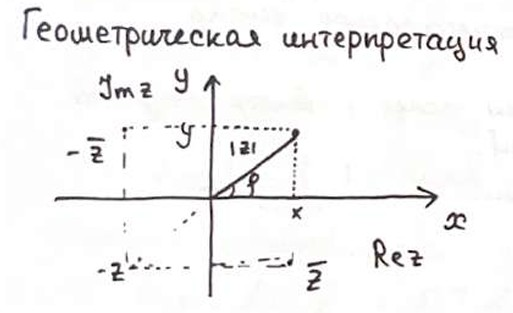
\includegraphics[scale=0.55]{images/module1/question01/1.jpg}
    \label{fig:picture_01_1}
\end{figure}


\begin{definition}
    \textbf{\textit{Модулем числа $z = x + iy$}} называется вещественное число $|z| = \sqrt{x^2 + y^2}$ (то есть длина соответствующего вектора).
\end{definition}

\textbf{Свойства.}

\begin{enumerate}[label={\arabic*°.}]
    \item $|z| \geq 0$, причем $|z| = 0 \iff z = 0$.
    \item $|z + w| \leq |z| + |w|$ (неравенство треугольника).

    Пусть $z = a + bi$, $w = c + di$.
    \begin{align*}
        |z + w| &\leq |z| + |w| \\
        \sqrt{(a + c)^2 + (b + d)^2} &\leq \sqrt{a^2 + b^2} + \sqrt{c^2 + d^2} \\
        (a + c)^2 + (b + d)^2 &\leq a^2 + b^2 + c^2 + d^2 + 2\sqrt{(a^2 + b^2)(c^2 + d^2)} \\
        ac + bd &\leq\sqrt{(a^2 + b^2)(c^2 + d^2)} \\
        ac + bd &\leq\sqrt{(ac)^2 + (ad)^2 + (bc)^2 + (bd)^2} \\
        (ac)^2 + (bd)^2 + 2acbd &\leq (ac)^2 + (ad)^2 + (bc)^2 + (bd)^2 \\
        2acbd &\leq (ad)^2 + (bc)^2 \\
        0 &\leq (ad)^2 + (bc)^2 - 2abcd \\
        0 &\leq (ad - bc)^2
    \end{align*}
    \item $z \overline{z} = |z|^2$.

    $z \overline{z} = (a + bi)(a - bi) = a^2 - (bi)^2 = a^2 + b^2 = |z|^2$
    \item $|zw| = |z||w|$.

    $|zw|^2 = (zw) \cdot (\overline{zw}) = z \cdot w \cdot \overline{z} \cdot \overline{w} = |z|^2 |w|^2$.
\end{enumerate}


\subsubsection*{
    Аргумент комплексного числа.
}


Пусть $z = a + bi \in \CC$, $z \neq 0$.

Тогда, $z = |z| \left(\frac{a}{|z|} + \frac{b}{|z|}i\right)$, при этом $\left(\frac{a}{|z|}\right)^2 + \left(\frac{b}{|z|}\right)^2 = (\frac{a}{\sqrt{a^2 + b^2}})^2 + (\frac{b}{\sqrt{a^2 + b^2}})^2 = \frac{a^2}{a^2 + b^2} + \frac{b^2}{a^2 + b^2} = \frac{a^2 + b^2}{a^2 + b^2} = 1.$

Значит, $\frac{a}{|z|}$ и $\frac{b}{|z|}$ являются синусом и косинусом некоторого угла.

\begin{definition}
    \textbf{\textit{Аргументом числа}} $z = a + bi \in \CC \setminus \{0\}$ называется любое число $\phi \in \RR$, такое что
    \begin{equation*}
        \cos \phi = \frac{a}{|z|} = \frac{a} {\sqrt{a^2 + b^2}}.
    \end{equation*}

    \begin{equation*}
        \sin \phi = \frac{b}{|z|} = \frac{b}{\sqrt{a^2 + b^2}}.
    \end{equation*}

    В геометрических терминах, $\phi$ есть угол между положительным направлением оси $Ox$ и вектором с началом в точке $0$ и концом в точке $z$.
\end{definition}

\begin{comment}
    Таких чисел бесконесно много, причем такие числа отличаются на $2\pi k, k \in \ZZ$.
\end{comment}


\newpage
\section{
    Линейные пространства. Определение, примеры. Базис и размерность пространства. Линейная оболочка системы векторов. Способы задания и переход между разными способами задания. Дать определение базиса и размерности линейного пространства. Связь между этими понятиями. Доказать теорему о единственности разложения вектора по базису. Привести пять примеров различных линейных пространств.
}

% Линейные пространства. Определение, примеры
\subsection{
    Линейные пространства. Определение, примеры.
}

\begin{definition}
    Непустое множество $\mathcal{L}$ называется \textbf{\textit{линейным пространством}} (афинным, векторным) над полем $\PP$, если $\forall \alpha, \beta \in \PP$ и $\forall \vec{a}, \vec{b} \in \mathcal{L}$ выполнены  линейность:  $(\alpha \vec{a} + \beta \vec{b}) \in \mathcal{L}$, и следующие аксиомы векторного пространства:

    \begin{enumerate}[nosep]
        \item $\vec{a} + \vec{b} = \vec{b} + \vec{a}$.
        \item $\forall \vec{c} \in \mathcal{L} \colon (\vec{a} + \vec{b}) + \vec{c} = \vec{a} + (\vec{b} + \vec{c})$.
        \item $\forall \vec{a} \thinspace \thinspace \exists \overrightarrow{0} \in \mathcal{L} \colon \vec{a} + \overrightarrow{0} = \vec{a}$.
        \item $\forall \vec{a} \thinspace \thinspace \exists \vec{a}' \in \mathcal{L} \colon \vec{a} + \vec{a'} = \overrightarrow{0}$.
        \item $(\alpha \beta) \vec{a} = \alpha(\beta \vec{a})$.
        \item $(\alpha + \beta)\vec{a} = \alpha \vec{a} + \beta \vec{a}$.
        \item $\alpha(\vec{a} + \vec{b}) = \alpha \vec{a} + \alpha \vec{b}$.
        \item $1 \cdot \vec{a} = \vec{a}$, $\forall \vec{a}$.
    \end{enumerate}
\end{definition}

\begin{definition}
    \textbf{\textit{Полем}} называется множество $\PP$ произвольной природы, на котором заданы две бинарные операции ($+$ и $\cdot$) и которое подчиняется следующим аксиомам:
    \begin{enumerate}[nosep]
        \item $\vec{a} + \vec{b} = \vec{b} + \vec{a}$.
        \item $\forall \vec{c} \colon (\vec{a} + \vec{b}) + \vec{c} = \vec{a} + (\vec{b} + \vec{c})$.
        \item $\forall \vec{a} \thinspace \thinspace \exists \overrightarrow{0} \in \PP \colon \vec{a} + \overrightarrow{0} = \vec{a}$.
        \item $\forall \vec{a} \thinspace \thinspace \exists \vec{a}' \in \PP \colon \vec{a} + \vec{a'} = \overrightarrow{0}$.
        \item $\vec{a} \cdot \vec{b} = \vec{b} \cdot \vec{a}$.
        \item $(\vec{a} \cdot \vec{b}) \cdot \vec{c} = \vec{a} \cdot (\vec{b} \cdot \vec{c})$.
        \item $\forall \vec{a} \thinspace \thinspace \exists \vec{e} \in \PP \thinspace \text{(\textbf{единичный})} \colon \vec{a} \cdot \vec{e} = \vec{a}$.
        \item $\forall \vec{a} \in \PP, \vec{a} \ne \vec{0} \thinspace \thinspace \exists \vec{a}^{-1} \in \PP \thinspace \colon \vec{a} \cdot \vec{a}^{-1} = \vec{e}$.
        \item $(\vec{a} + \vec{b}) \cdot \vec{c} = (\vec{a} \cdot \vec{c}) + (\vec{b} \cdot \vec{c})$.
    \end{enumerate}
\end{definition}

\begin{definition}
    Элементы линейного пространства называются (абстрактными) \textbf{\textit{векторами}}.
\end{definition}

\begin{example}~
    \begin{itemize}[nosep]
        \item множество $\mathcal{V}_3 (\mathcal{V}_2)$ всех \textit{свободных векторов} в пространстве (на плоскости) с линейными операциями над векторами - линейное пространство.
        
        \item множество всех \textit{геометрических векторов} в пространстве с началом в данной точке и параллельных данной плоскости (рис. \ref{fig:picture_02_1}) с линейными операциями над векторами.
        \begin{figure}[H]
            \centering
            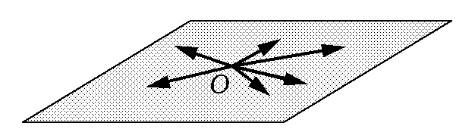
\includegraphics[scale=0.5]{images/module1/question02/1.jpg}
            \label{fig:picture_02_1}
            \caption{}
        \end{figure}

        \item множество $M_{mn}(\RR)$ матриц типа $m \times n$, элементами которых являются действительные числа, с линейными операциями над матрицами.

        \item множество $K_n[x]$ многочленов переменного $x$ степени, не превышающей $n$, которые как функции можно складывать и умножать на действительные числа.

        \item множество всех решений данной ОСЛАУ (решения можно рассматривать как матрицы-столбцы, складывать и умножать на числа по законам матричных операций).

        \item множество функций, непрерывных на отрезке, с обычными операциями сложения функций и умножения функции на число.

        \item $\RR$ является линейным пространством над полем $\QQ$.
        
        \item $\CC$ является линейным пространством над полем $\RR$.
    \end{itemize}
\end{example}



\newpage


% Базис и размерность пространства
\subsection{
    Базис и размерность пространства.
}

\begin{definition}
    \textbf{\textit{Базисом линейного пространства}} $\mathcal{L}$ называют любую упорядоченную систему векторов, для которой выполнены два условия:
    \begin{enumerate}[nosep]
        \item эта система векторов линейно независима.
        \item каждый вектор в линейном пространстве может быть представлен в виде линейной комбинации векторов этой системы.
    \end{enumerate}
\end{definition}

\begin{definition}
    Максимальное количество линейно независимых векторов в данном линейном пространстве называют \textbf{\textit{размерностью линейного пространства}}.
\end{definition}

\begin{designation}
    $n = \dim \mathcal{L}$, где $n$ - размерность линейного пространства $\mathcal{L}$.
\end{designation}



\newpage


% Связь между базисом и размерностью пространства
\subsection{
    Связь между базисом и размерностью пространства.
}

\begin{theorem}
    Если $\dim \mathcal{L} = n$, то любая линейно независимая система из $n$ векторов является его базисом.
    \label{thm:theorem_2_1}
\end{theorem}

\begin{proof}~

    Пусть система векторов $\vec{b_1}, \ldots, \vec{b_n} \in \mathcal{L}$ линейно независима. Тогда для любого вектора $\vec{x} \in \mathcal{L}$ система векторов $\vec{x}, \vec{b_1}, \ldots, \vec{b_n}$ линейно зависима, так как она содержит $n + 1$ вектор, т.е. количество большее, чем размерность линейного пространства. Это значит, что существуют такие коэффициенты $\alpha_0, \alpha_1, \ldots, \alpha_n$, одновременно не равные нулю, что

    \begin{equation}
        \alpha_0\vec{x} + \alpha_1\vec{b_1} + \ldots + \alpha_n\vec{b_n} = \vec{0}
        \label{eq:theorem_2_1_1}
    \end{equation}

    Заметим, что $\alpha_0 \ne 0$, так как в противном случае равенство \eqref{eq:theorem_2_1_1} сводится к равенству

    \begin{equation}
        \alpha_1\vec{b_1} + \ldots + \alpha_n\vec{b_n} = \vec{0},
    \end{equation}

    причем среди коэффициентов $\alpha_1, \ldots, \alpha_n$ есть хотя бы один ненулевой (так как $\alpha_0 = 0$). Но это означало бы, что система векторов $\vec{b_1}, \ldots, \vec{b_n}$ линейно зависима. 
    
    Учитывая, что $\alpha_0 \ne 0$, из \eqref{eq:theorem_2_1_1} находим

    \begin{equation}
        \vec{x} = -\frac{\alpha_1}{\alpha_0}\vec{b_1} - \ldots - \frac{\alpha_n}{\alpha_0}\vec{b_n}.
    \end{equation}

    Так как вектор $\vec{x}$ был выбран произвольно, заключаем, что любой вектор в линейном пространстве $\mathcal{L}$ можно представить в виде линейной комбинации системы векторов $\vec{b_1}, \ldots, \vec{b_n}$.

    Поэтому эта система векторов, по предположению линейно независимая, является базисом в $\mathcal{L}$.
\end{proof}

\begin{theorem}[обратная]
    Если в линейном пространстве $\mathcal{L}$ существует базис из $n$ векторов, то $\dim \mathcal{L} = n$.
    \label{thm:theorem_2_2}
\end{theorem}


\newpage


% Теорема о единственности разложения вектора по базису
\subsection{
    Теорема о единственности разложения вектора по базису.
}

\begin{theorem}
    В линейном пространстве разложение любого вектора по данному базису единственно.
    \label{thm:theorem_2_3}
\end{theorem}

\begin{proof}
    Выберем в линейном пространстве $\mathcal{L}$ произвольный базис $\vec{b_1}, \ldots, \vec{b_n}$ и предположим, что вектор $\vec{x}$ имеет в этом базисе два разложения
    \begin{align*}
        \vec{x} = x_1\vec{b_1} + \ldots + x_n\vec{b_n},\\
        \vec{x} = x_1'\vec{b_1} + \ldots + x_n'\vec{b_n}.
    \end{align*}
    Воспользуемся тем, что аксиомы линейного пространства позволяют преобразовывать линейные комбинации так же, как и обычные алгебраические выражения. Вычитая записанные равенства почленно, получим
    $$(x_1 - x_1')\vec{b_1} + \ldots + (x_n - x_n')\vec{b_n} = 0$$
    Так как базис - это линейно независимая система векторов, ее линейная комбинация равна $0$, лишь если она тривиальная. Значит, все коэффициенты этой линейной комбинации равны нулю: $x_1 - x_1' = 0, \ldots, x_n - x_n' = 0$. Таким образом, $x_1 = x_1', \ldots, x_n = x_n'$ и два разложения вектора $\vec{x}$ в базисе $\vec{b_1}, \ldots, \vec{b_n}$ совпадают.
\end{proof}



\newpage


% Линейная оболочка системы векторов. Способы задания линейного подпространства и переход между разными способами задания
\subsection{
    Линейная оболочка системы векторов. Способы задания линейного подпространства и переход между разными способами задания.
}

\begin{definition}
    \textbf{\textit{Линейной оболочкой}} системы векторов $\vec{a_1}, \ldots, \vec{a_n}$ называется множество всех линейных комбинаций этой системы.
\end{definition}

\begin{theorem}
    Линейная оболочка является линейным пространством.
\end{theorem}

\begin{designation}
    $\Span(\vec{a_1}, \ldots, \vec{a_n})$.
\end{designation}

Существует 2 способа задания линейного подпространства:

\begin{enumerate}
    \item явное - $\mathcal{L} = \Span(\vec{a_1}, \ldots, \vec{a_k})$.
    \item неявное - $\mathcal{L}$ - решение однородной СЛАУ.
\end{enumerate}

\subsection*{Переход между разными способами задания.
}

\begin{itemize}
    \item Если подпространство задано неявно, то для перехода к явному способу достаточно решить однородную систему уравнений, выбрав какую-либо ФСР. Столбцы ФСР - это столбцы координат векторов некоторого базиса рассматриваемого подпространства. Следовательно, подпространство можно задать как линейную оболочку системы этих векторов.
    \item Опишем два способа перехода от явного описания к неявному.

    \begin{enumerate}
        \item Выберем в линейном пространстве какой-либо базис и запишем векторы заданной системы векторов $\vec{a}_1, \vec{a}_2, \ldots, \vec{a}_k$ через координаты в выбранном базисе. Вектор $\vec{b}$ с координатами $b = \begin{pmatrix}
            b_1 \\
            b_2 \\
            \vdots \\
            b_n
        \end{pmatrix}$ является линейной комбинацией заданной системы векторов тогда и только тогда, когда СЛАУ $\begin{pmatrix}
            \vec{a}_1 & \vec{a}_2 & \ldots & \vec{a}_k & \vec{b}
        \end{pmatrix}$ совместна. Записывая условие совместности с помощью теоремы Кронекера-Капелли, получим уравнения, связывающие координаты вектора $\vec{b}$. Эти уравнения составляют СЛАУ, неявно описывающую подпространство $\mathcal{H} = \Span(\vec{a}_1, \vec{a}_2, \ldots, \vec{a}_k)$.
    
    \item Пусть $\mathcal{H} = \Span(\vec{a}_1, \vec{a}_2, \ldots, \vec{a}_k)$. Составим матрицу $A$ из столбцов координат векторов $\vec{a}_1, \vec{a}_2, \ldots, \vec{a}_k$ в некотором базисе. Решим однородную СЛАУ $A^T\vec{x} = \vec{0}$, найдя какую-либо ФСР этой СЛАУ. Из столбцов ФСР составим матрицу $F$. Однородная СЛАУ $F^T\vec{x} = \vec{0}$ неявно описывает подпространство $\mathcal{H}$.
    \end{enumerate}
\end{itemize}


\newpage
\section{
    Линейные подпространства. Определения, теоремы, примеры и контрпримеры. Базис и размерность. Привести примеры задания пространств и подпространств без использования матриц и СЛАУ.
}

% Линейные подпространства. Определения, теоремы, примеры и контрпримеры
\subsection{
    Линейные подпространства. Определения, теоремы, примеры и контрпримеры.
}

\begin{definition}
    Подмножество $\mathcal{L}_1 \subset \mathcal{L}$ называется \textbf{\textit{линейным подпространством}} над полем $\PP$, если \\ $\forall \vec{a}, \vec{b} \in \mathcal{L}_1, \forall \alpha, \beta \in \PP \colon \alpha \vec{a} + \beta \vec{b} \in \mathcal{L}$.
\end{definition}

\begin{theorem}
    Линейное подпространство является линейным пространством.
\end{theorem}

\begin{example}~

    \begin{enumerate}
        \item В любом линейном пространстве $\mathcal{L}$ всегда имеются два линейных подпространства: само пространство $\mathcal{L}$ и нулевое подпространство, состоящее из одного нулевого элемента. Эти подпространства называются \textbf{\textit{несобственными}}. Все остальные линейные пространства называются \textbf{\textit{собственными}}.
        \item Множество всех свободных векторов, параллельных данной плоскости, образуют линейное подпространство пространства $\mathcal{V}_3$ всех свободных векторов трехмерного пространства.
        \item В линейном пространстве $M_n(\RR)$ всех квадратных матриц порядка $n$ линейное подпространство образуют все симметрические матрицы.
    \end{enumerate}
\end{example}

\begin{counterexample}~

    \begin{enumerate}
        \item Множество всех векторов на плоскости, у которых первая координата положительна. Это множество не является подпространством, потому что оно не замкнуто относительно умножения на скаляр. Например, вектор $(1, 1)$ принадлежит этому множеству, но вектор $-1 \cdot (1, 1) = (-1, -1)$ — нет, так как первая координата отрицательна.
        \item Множество всех векторов в $\RR^3$, лежащих в первой октанте (где все координаты неотрицательны). Это множество не замкнуто относительно умножения на скаляр. Например, вектор $(1, 1, 1)$ принадлежит этому множеству, но вектор $-1 \cdot (1, 1, 1) = (-1, -1, -1)$ не принадлежит.
    \end{enumerate}
\end{counterexample}



\newpage


% Базис и размерность
\subsection{
    Базис и размерность.
}

\begin{definition}
    \textbf{\textit{Базисом линейного подпространства}} $\mathcal{L}$ называют любую упорядоченную систему векторов, для которой выполнены два условия:
    \begin{enumerate}[nosep]
        \item эта система векторов линейно независима.
        \item каждый вектор в линейном подпространстве может быть представлен в виде линейной комбинации векторов этой системы.
    \end{enumerate}
\end{definition}

\begin{definition}
    Максимальное количество линейно независимых векторов в данном линейном подпространстве называют \textbf{\textit{размерностью линейного подпространства}}.
\end{definition}



\newpage


% Привести примеры задания пространств и подпространств без использования матриц и СЛАУ
\subsection{
    Привести примеры задания пространств и подпространств без использования матриц и СЛАУ.
}

\begin{enumerate}
    \item В любом линейном пространстве $\mathcal{L}$ всегда имеются два линейных подпространства: само пространство $\mathcal{L}$ и нулевое подпространство, состоящее из одного нулевого элемента.
    \item Множество всех свободных векторов, параллельных данной плоскости, образуют линейное подпространство пространства $\mathcal{V}_3$ всех свободных векторов трехмерного пространства.
    \item Любая прямая, проходящая через начало координат $(0, 0, 0)$ в $\RR^3$.
    \item Линейное пространство - множество $P_n[x]$ многочленов переменного $x$ степени, не превышающей $n$. Для данного линейного пространства линейным подпространтсвом является множество $K_m[x]$ многочленов переменного $x$ степени, не превышающей $m$, где $m \leq n$. При этом подпространством не является множество всех многочленов степени ровно $m$. Например, сумма двух многочленов степени $m$ может иметь степень меньше $m$ (например, x² + (-x²) = 0).
    \item Множество функций, непрерывных на отрезке, с обычными операциями сложения функций и умножения функции на число.
\end{enumerate}


\newpage
\section{
    Сумма и пересечение линейных подпространств. Доказать, что указанные множества являются линейными подпространствами. Нахождение базисов для суммы и пересечения подпространств. Теорема о размерностях подпространств, суммы и пересечения.
}

% Сумма и пересечение линейных подпространств
\subsection{
    Сумма и пересечение линейных подпространств.
}   

\begin{definition}
    Пусть $\mathcal{H}_1$ и $\mathcal{H}_2$ - линейные подпространства в линейном пространстве $\mathcal{L}$. Множество $\mathcal{H}_1 + \mathcal{H}_2$ всех векторов $\vec{x}$ вида $\vec{x} = \vec{x_1} + \vec{x_2}$, где $\vec{x_1} \in \mathcal{H}_1$, $\vec{x_2} \in \mathcal{H}_2$, называют \textbf{\textit{суммой линейных подпространств}} $\mathcal{H}_1$ и $\mathcal{H}_2$. 
\end{definition}

\begin{figure}[H]
    \centering
    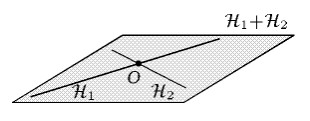
\includegraphics[scale=0.7]{images/module1/question04/1.jpg}
    \label{fig:picture_04_1}
    \caption{Сумма линейных подпространств.}
\end{figure}

\begin{definition}
    Пусть $\mathcal{H}_1$ и $\mathcal{H}_2$ - линейные подпространства в линейном пространстве $\mathcal{L}$. Множество $\mathcal{H}_1 \cap \mathcal{H}_2$ всех векторов $\vec{x}$, где $\vec{x} \in \mathcal{H}_1$ и $\vec{x} \in \mathcal{H}_2$, называют \textbf{\textit{пересечением линейных подпространств}} $\mathcal{H}_1$ и $\mathcal{H}_2$.
\end{definition}

\begin{figure}[H]
    \centering
    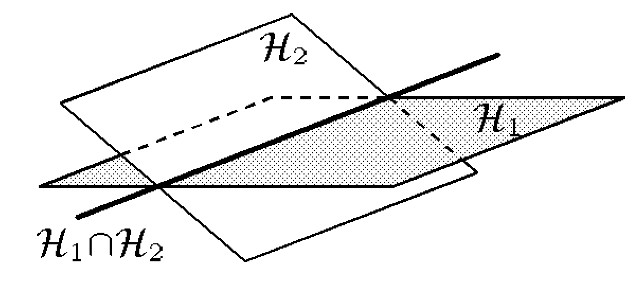
\includegraphics[scale=0.4]{images/module1/question04/2.jpg}
    \label{fig:picture_04_2}
    \caption{Пересечение линейных подпространств.}
\end{figure}




\newpage


% Доказать, что указанные множества (сумма и пересечение ЛПП) являются линейными подпространствами
\subsection{
    Доказать, что указанные множества (сумма и пересечение ЛПП) являются линейными подпространствами.
}

\begin{theorem}
    Сумма линейных подпространств данного линейного пространства является линейным подпространством в том же линейном пространстве.
\end{theorem}

\begin{proof}~

    Проверим, выполняются ли условия определения линейного подпространства:
    \begin{enumerate}[nosep]
        \item Рассмотрим два вектора $\vec{v}$ и $\vec{w}$ из множества $\mathcal{H}_1 + \mathcal{H}_2$. Согласно определению суммы линейных подпространств, имеют место представления $\vec{v} = \vec{x_1} + \vec{x_2}$, $\vec{w} = \vec{y_1} + \vec{y_2}$, где векторы $\vec{x_i}$, $\vec{y_i}$ принадлежат $\mathcal{H}_i$, $i = 1, 2$. Складывая эти равенства, получаем
        $$\vec{v} + \vec{w} = (\vec{x_1} + \vec{y_1}) + (\vec{x_2} + \vec{y_2}).$$
        Сумма $\vec{x_1} + \vec{y_1}$ векторов $\vec{x_1}$ и $\vec{y_1}$ линейного подпространства $\mathcal{H}_1$ принадлежит $\mathcal{H}_1$. Точно так же сумма $\vec{x_2} + \vec{y_2}$ векторов $\vec{x_2}$ и $\vec{y_2}$ линейного подпространства $\mathcal{H}_2$ принадлежит $\mathcal{H}_2$. Поэтому вектор $\vec{v} + \vec{w}$ принадлежит множеству $\mathcal{H}_1 + \mathcal{H}_2$.
        \item Произвольный вектор $\vec{v} \in \mathcal{H}_1 + \mathcal{H}_2$ имеет представление $\vec{v} = \vec{x_1} + \vec{x_2}$, где $\vec{x_1} \in \mathcal{H}_1$, $\vec{x_2} \in \mathcal{H}_2$. Для любого действительного числа $\lambda$ получаем равенства 
        $$\lambda \vec{v} = \lambda (\vec{x_1} + \vec{x_2}) = \lambda \vec{x_1} + \lambda \vec{x_2}.$$
        Так как вектор $\lambda \vec{x_1}$ принадлежит $\mathcal{H}_1$, а вектор $\lambda \vec{x_2}$ - $\mathcal{H}_2$, то вектор $\lambda \vec{u}$ является элементом множества $\mathcal{H}_1 + \mathcal{H}_2$.
    \end{enumerate}
    Мы доказали, что множество $\mathcal{H}_1 + \mathcal{H}_2$ замкнуто относительно линейных операций объемлющего линейного пространства и поэтому, согласно определению линейного подпространства, оно является линейным подпространством.
\end{proof}

\begin{theorem}
    Пересечение $\mathcal{H}_1 \cap \mathcal{H}_2$ двух линейных подпространств $\mathcal{H}_1$ и $\mathcal{H}_2$ в линейном пространстве $\mathcal{L}$ является линейным подпространством в $\mathcal{L}$.
\end{theorem}

\begin{proof}~

    Проверим, выполняются ли условия определения линейного подпространства:
    \begin{enumerate}[nosep]
        \item Если векторы $\vec{x_1}$ и $\vec{x_2}$ принадлежат $\mathcal{H}_1 \cap \mathcal{H}_2$, то каждый из этих векторов принадлежит как $\mathcal{H}_1$, так и $\mathcal{H}_2$. Поскольку $\mathcal{H}_1$ - линейное подпространство, то согласно определению линейного подпространства, заключаем, что вектор $\vec{x_1} + \vec{x_2}$, равный сумме векторов этого линейного подпространства, тоже принадлежит $\mathcal{H}_1$. Аналогично $\vec{x_1} + \vec{x_2} \in \mathcal{H}_2$, так как каждое из слагаемых является элементом линейного подпространства $\mathcal{H}_2$. Следовательно, $\vec{x_1} + \vec{x_2} \in \mathcal{H}_1 \cap \mathcal{H}_2$.
        \item Выберем произвольный вектор $\vec{x} \in \mathcal{H}_1 \cap \mathcal{H}_2$. Тогда $\vec{x} \in \mathcal{H}_1$ и $\vec{x} \in \mathcal{H}_2$. Так как $\mathcal{H}_1$ является линейным подпространством, то произведение элемента $\vec{x}$ этого линейного подпространства на произвольное действительное число $\lambda$ принадлежит $\mathcal{H}_1$. Но совершенно аналогично вектор $\lambda \vec{x}$ принадлежит и $\mathcal{H}_2$. Поэтому $\lambda \vec{x} \in \mathcal{H}_1 \cap \mathcal{H}_2$. 
    \end{enumerate}
    Итак, оба условия определения линейного подпространства выполнены. Следовательно, $\mathcal{H}_1 \cap \mathcal{H}_2$ является линейным подпространством.
\end{proof}



\newpage

% Нахождение базисов для суммы и пересечения подпространств
\subsection{
    Нахождение базисов для суммы и пересечения подпространств.
}

\begin{theorem}
    Если $\{e\}$ - базис $\mathcal{L}_1$, $\{f\}$ - базис $\mathcal{L}_2$, $\ldots$, $\{g\}$ - базис $\mathcal{L}_k$, то $\sum_{j=1}^{k} L_j = span(e, f, \ldots, g)$.
\end{theorem}

\begin{proof}
    $\vec{x} = \underbrace{\vec{x_1}}_{\text{расклад. по $e$}} + \underbrace{\vec{x_2}}_{\text{расклад. по $f$}} + \ldots + \underbrace{\vec{x_k}}_{\text{расклад. по $g$}}$
\end{proof}

\begin{comment}
    Набор $(e, f, \ldots, g)$ может быть избыточен; нужны только ЛНЗ векторы.
\end{comment}

\begin{proposition}
    $\dim \sum_{j=1}^{k} \mathcal{L}_j = rank(e, f, \ldots, g)$.
\end{proposition}

Пусть $\mathcal{L}_1, \mathcal{L}_2, \ldots, \mathcal{L}_k$ заданы с помощью СЛАУ. Базисом суммы подпространств $\mathcal{L}_1 + \mathcal{L}_2 + \ldots + \mathcal{L}_k$ будет любая её ФСР. Базисом пересечения подпространств $\mathcal{L}_1 \cap \mathcal{L}_2 \cap \ldots \cap \mathcal{L}_k$ будет любая его ФСР.



\newpage


% Теорема о размерностях подпространств, суммы и пересечения
\subsection{
    Теорема о размерностях подпространств, суммы и пересечения.
}

\begin{theorem}
    Если $\mathcal{H}$ - линейное подпространство линейного пространства $\mathcal{L}$, то $\dim \mathcal{H} \leq \dim \mathcal{L}$. Если к тому же $\mathcal{H} \ne \mathcal{L}$, то $\dim \mathcal{H} < \dim \mathcal{L}$.
\end{theorem}

\begin{proof}~

    Любой базис линейного подпространства $\mathcal{H}$ является ЛНЗ системой векторов в линейном пространстве $\mathcal{L}$. Если этот базис из $\mathcal{H}$ является базисом и в $\mathcal{L}$, то согласно теореме \eqref{thm:theorem_2_2}, $\dim \mathcal{H} = \dim \mathcal{L}$ и ясно, что в этом случае $\mathcal{H} = \mathcal{L}$, так как у них общий базис. Если базис $\mathcal{H}$ не является базисом $\mathcal{L}$, то $\exists \vec{x} \in \mathcal{L}$, который не является линейной комбинацией векторов этого базиса $\implies \mathcal{H} \ne \mathcal{L}$. Добавив вектор $x$ к векторам базиса, получим ЛНЗ систему векторов. Значит, в $\mathcal{L}$ больше ЛНЗ векторов, чем в $\mathcal{H} \implies \dim \mathcal{H} < \dim \mathcal{L}$.
\end{proof}

\begin{theorem}
    Если $\mathcal{H}_1$ и $\mathcal{H}_2$ - линейные подпространства линейного пространства $\mathcal{L}$, то
    $$\dim(\mathcal{H}_1 + \mathcal{H}_2) = \dim\mathcal{H}_1 + \dim\mathcal{H}_2 - \dim(\mathcal{H}_1 \cap \mathcal{H}_2).$$
    \label{thm:theorem_4_6}
\end{theorem}

\begin{proof}~

    В линейном подпространстве $\mathcal{H}_1 \cap \mathcal{H}_2$ выберем некоторый базис $\vec{e} = (\vec{e_1}, \ldots, \vec{e_m})$. Множество $\mathcal{H}_1 \cap \mathcal{H}_2$ является линейным подпространством не только в $\mathcal{L}$, но и в его части $\mathcal{H}_1$. Поэтому выбранный базис можно дополнить некоторой системой векторов $f = (\vec{f_1}, \ldots, \vec{f_l})$ до базиса $(e, f)$ в линейном подпространстве $\mathcal{H}_1$. Аналогично систему $e$ можно дополнить некоторым набором векторов $g = (\vec{g_1}, \ldots, \vec{g_k})$ до базиса $(e, g)$ в $\mathcal{H}_2$. Докажем, что система векторов
    $$(e, f, g) = (\vec{e_1}, \ldots, \vec{e_m}, \vec{f_1}, \ldots, \vec{f_l}, \vec{g_1}, \ldots, \vec{g_k})$$
    является базисом в линейном пространстве $\mathcal{H}_1 + \mathcal{H}_2$.

    \textbf{Во-первых}, установим, что указанная система линейно независима. Пусть имеет место равенство
    $$\alpha_1\vec{e_1} + \ldots + \alpha_m\vec{e_m} + \beta_1\vec{f_1} + \ldots + \beta_l\vec{f_l} + \gamma_1\vec{g_1} + \ldots \gamma_k\vec{g_k} = \vec{0}$$
    Тогда для вектора
    \begin{equation}
        \vec{y} = \beta_1\vec{f_1} + \ldots + \beta_l\vec{f_l}.
        \label{eq:theorem_4_6_1}
    \end{equation}
    выполнено равенство
    \begin{equation}
        \vec{y} = -\alpha_1\vec{e_1} - \ldots -\alpha_m\vec{e_m} - \gamma_1\vec{g_1} - \ldots - \gamma_k\vec{g_k}.
        \label{eq:theorem_4_6_2}
    \end{equation}
    Согласно равенству \eqref{eq:theorem_4_6_1} заключаем, что $\vec{y} \in \mathcal{H}_1$, а согласно \eqref{eq:theorem_4_6_2} делаем вывод, что $\vec{y} \in \mathcal{H}_2$. Следовательно, $\vec{y} \in \mathcal{H}_1 \cap \mathcal{H}_2$ и потому имеет единственное разложение
    \begin{equation}
        \vec{y} = \delta_1\vec{e_1} + \ldots + \delta_m\vec{e_m}.
        \label{fig:theorem_4_6_3}
    \end{equation}
    по базису $e$ линейного пространства $\mathcal{H}_1 \cap \mathcal{H}_2$.

    Рассмотрев разложение по $(e, g)$ и $(e, f)$, получим, что все коэффициенты равны нулю. Значит, система векторов $(e, f, g)$ линейно независима.

    \textbf{Во-вторых}, всякий вектор $\vec{y} \in \mathcal{H}_1 + \mathcal{H}_2$ есть линейная комбинация системы векторов $(e, f, g)$. Действительно, такой вектор представим в виде $\vec{y} = \vec{y_1} + \vec{y_2}$, где $\vec{y_1} \in \mathcal{H}_1$, $\vec{y_2} \in \mathcal{H}_2$. Вектор $\vec{y_1}$ представляется линейной комбинацией системы векторов $(e, f)$, а $\vec{y_2}$ - линейной комбинацией системы векторов $(e, g)$. Поэтому $\vec{y}$ разлагается по системе векторов $(e, f, g)$.

    Итак, система векторов $(e, f, g)$ линейно независима и любой вектор из $\mathcal{H}_1 + \mathcal{H}_2$ разлагается по этой системе. Следовательно, $(e, f, g)$ - базис $\mathcal{H}_1 + \mathcal{H}_2$. Остается подсчитать размерности:
    
    \begin{table}[H]
        \centering
        \begin{tabular}{|c|c|c|}
            \hline
            Линейное подпространство & базис & размерность\\
            \hline
            $\mathcal{H}_1$ & $(e, f)$ & $m + l$\\
            \hline
            $\mathcal{H}_2$ & $(e, g)$ & $m + k$\\
            \hline
            $\mathcal{H}_1 \cap \mathcal{H}_2$ & $e$ & $m$\\
            \hline
            $\mathcal{H}_1 + \mathcal{H}_2$ & $(e, f, g)$ & $m + l + k$\\
            \hline
        \end{tabular}
        \label{tab:my_label}
    \end{table}
    Таким образом, получаем утверждение теоремы.
\end{proof}

\begin{corollary}
    $\dim(\mathcal{H}_1 \oplus \mathcal{H}_2) = \dim \mathcal{H}_1 + \dim \mathcal{H}_2.$
    \label{cor:corollary_4_6}
\end{corollary}


\newpage
\section{
    Прямая сумма подпространств. Критерий прямой суммы.
}

% Прямая сумма подпространств. Критерий прямой суммы
\begin{definition}
    Сумма линейных подпространств $\mathcal{H}_1, \mathcal{H}_2, \ldots, \mathcal{H}_j$ данного пространства $\mathcal{H}$ называется \textbf{\textit{прямой суммой}}, если представление любого ее вектора $\vec{x} = \vec{x}_1 + \vec{x}_2 + \ldots + \vec{x}_j, \vec{x}_j \in \mathcal{H}_j$ - единственно.
\end{definition}

\begin{designation}
    $\mathcal{H}_1 \oplus \mathcal{H}_2 \oplus \ldots \oplus \mathcal{H}_j = \mathcal{H}$.
\end{designation}

\begin{theorem}[Критерий прямой суммы]
    Для линейных подпространств $\mathcal{L}_1, \ldots, \mathcal{L}_k$ конечномерного пространства $\mathcal{L}$ следующие утверждения равносильны:
    \begin{enumerate}
        \item Сумма $\mathcal{L}_1, \ldots, \mathcal{L}_k$ - прямая.
        \item Совокупность их базисов линейно независима.
        \item Совокупность базисов образует базис суммы.
        \item Размерность суммы равна сумме размерностей $\mathcal{L}_j$.
        \item В сумме существует хотя бы один вектор с единственным разложением по подпространством.
        \item Произвольная система $\vec{x}_j \in \mathcal{L}_j$, взятых по одному из любого $\mathcal{L}_j$, линейно независима.
        \item Только для $k = 2$, т.е. $\mathcal{L}_1$ и $\mathcal{L}_2$, $\mathcal{L}_1 \cap \mathcal{L}_2 = \vec{0}$.
    \end{enumerate}
\end{theorem}

\begin{proof}~

    $1 \to 2$: Предположим, что линейно зависима $\Rightarrow$ разложение не единственно, т.е. $\vec{0} = \alpha_1(\vec{x}_1 - \vec{x}_1') + \ldots + \alpha_n(\vec{x}_n - \vec{x}_n')$, что противоречит определению прямой суммы.

    \bigbreak

    $2 \to 3$: Совокупность базисов линейно независима и каждый вектор имеет единственное разложение, то есть совокупность базисов является базисом.

    \bigbreak

    $3 \to 4$: суммируем базисы $\dim \Sigma \mathcal{L}_j = \Sigma \dim \mathcal{L}_j$.

    \bigbreak

    $4 \to 5$: От противного $\Rightarrow$ линейная зависимость векторов базиса.

    \bigbreak

    $5 \to 6$: $\vec{x} = \vec{x}_1 + \ldots + \vec{x}_k$, предположим линейную зависимость, т.е. $\alpha_1\vec{x}_1 + \ldots + \alpha_k\vec{x}_k = \vec{0}$

    $\vec{x} + \vec{0} = \vec{x}$ - не единственное.

    \bigbreak

    $6 \to 1$: $\vec{x}_1,\ldots,\vec{x}_k$ линейно независима $\Rightarrow$ сумма подпространств $\mathcal{L}_1, \ldots, \mathcal{L}_k$ прямая. Предположим обратное. 

    $\vec{x} = \alpha_1\vec{x}_1 + \ldots + \alpha_k\vec{x}_k$,
    
    $\vec{x} = \beta_1\vec{x}_1 + \ldots + \beta_k\vec{x}_k$

    То есть $\vec{x}_1,\ldots,\vec{x}_k$ линейно зависимы - противоречие.

    \bigbreak

    $7\leftrightarrow 4$: значит, $\dim \mathcal{L}_1 \cap \mathcal{L}_2 = \vec{0}$.
\end{proof}


\newpage
\section{
    Линейное аффинное многообразие. Вектор сдвига. Пересечение линейных аффинных многообразий. 
}

% Линейное аффинное многообразие. Вектор сдвига
\subsection{
    Линейное аффинное многообразие. Вектор сдвига.
}

\begin{definition}
    Пусть $\mathcal{V}$ - линейное пространство над полем $\PP$, $\mathcal{W}$ - это его подпространство. Зафиксируем вектор $\vec{a} \in \mathcal{V}$. Тогда множество $\vec{a} + \mathcal{W} = \{\, \vec{a} + \vec{x} \mid \vec{x} \in \mathcal{W} \,\}$ называется \textbf{\textit{линейным аффинным многообразием}}.

    При этом подпространство $\mathcal{W}$ называется \textbf{\textit{направляющим подпространством}}, а вектор $\vec{a}$ называется \textbf{\textit{вектором сдвига}}.
\end{definition}

Заметим, что ЛАМ, вообще говоря, не является подпространством (например, потому что оно может не содержать $\vec{0} \in \mathcal{V}$.)

\begin{proof}~

    Если $\vec{a} \notin \mathcal{W}$, то согласно аксиоме линейного пространства, и $(-\vec{a}) \notin \mathcal{W}$. 

    \begin{gather*}
        \text{Предположим, что } \underbrace{\vec{a} + (-\vec{a})}_{\vec{0}} \in \vec{a} + \mathcal{W}. \\
        \exists \vec{w} \in \mathcal{W} (\vec{a} + (-\vec{a}) = \vec{a} + \underbrace{\vec{w}}_{\in \mathcal{W}}). \\
        \exists \vec{w} \in \mathcal{W} ((-\vec{a}) = \vec{w}). \\
        \downimplies \\
        -\vec{a} \notin \mathcal{W}\text{. Противоречие.}
    \end{gather*}
    Это и означает, что если $\vec{a} \notin \mathcal{W}$, то $\vec{a} + \mathcal{W}$ не является подпространством.
\end{proof}

\begin{definition}
    \textbf{\textit{Размерностью}} линейного аффинного многообразия $\vec{a} + \mathcal{W}$ называется размерность $\mathcal{W}$, т.е. $$\dim (\vec{a} + \mathcal{W}) = \dim \mathcal{W}.$$
\end{definition}

\begin{definition}
    Пусть 

    \begin{enumerate}
        \item $\mathcal{V}$ - линейное пространство,
        \item $\dim \mathcal{V} = n$,
        \item $\mathcal{W}$ - некоторое подпространство $\mathcal{V}$.
    \end{enumerate}
    
    Тогда \textbf{\textit{гиперплоскостью}} в нем будет называться ЛАМ вида $(\vec{a} + \mathcal{W})$, где $\dim \mathcal{W} = n - 1$.
\end{definition}



\newpage


% Пересечение линейных аффинных многообразий
\subsection{
    Пересечение линейных аффинных многообразий.
}

\begin{theorem}
    Пересечение двух линейных аффинных многообразий одного линейного пространства либо пусто, либо является линейным аффинным многообразием.
\end{theorem}

\begin{proof}~

    Пусть дано линейное пространство $\mathcal{V}$, в нем есть некоторые линейные подпространства $\mathcal{U}$ и $\mathcal{W}$. Зафиксируем $\vec{a}, \vec{b} \in \mathcal{V}$. Тогда возникают ЛАМ-я $(\vec{a} + \mathcal{U})$ и $(\vec{b} + \mathcal{W})$.

    Рассмотрим их пересечение $(\vec{a} + \mathcal{U}) \cap (\vec{b} + \mathcal{W})$.

    \textbf{1 случай}: $(\vec{a} + \mathcal{U}) \cap (\vec{b} + \mathcal{W}) = \emptyset$.

    Тогда всё доказано. Достаточно привести пример, когда действительно $(\vec{a} + \mathcal{U}) \cap (\vec{b} + \mathcal{W}) = \emptyset$.

    \bigbreak

    \textbf{2 случай}: $(\vec{a} + \mathcal{U}) \cap (\vec{b} + \mathcal{W}) \ne \emptyset$.

    Зафиксируем некоторый вектор $\vec{c} \in \vec{a} + \mathcal{U}$ и $\vec{c} \in \vec{b} + \mathcal{W}$, т.е. $\vec{c} = \vec{a} + \underbrace{\vec{u}}_{\in \mathcal{U}} = \vec{b} + \underbrace{\vec{w}}_{\in \mathcal{W}}$.

    Докажем, что $(\vec{a} + \mathcal{U}) \cap (\vec{b} + \mathcal{W}) = \vec{c} + \underbrace{(\mathcal{U} \cap \mathcal{W})}_{\text{явл. ЛПП } \mathcal{V}.}$.

    \begin{enumerate}
        \item[$\subseteq$] Рассмотрим произвольный вектор $\vec{\varphi} = \vec{a} + \underbrace{\vec{x}}_{\in \mathcal{U}} =\vec{b} + \underbrace{\vec{y}}_{\in \mathcal{W}}.$
    
        Докажем, что он лежит в $\vec{c} + (\mathcal{U} \cap \mathcal{W})$.
    
        $$\vec{\varphi} = \vec{a} + \vec{x} = (\vec{a} + \vec{u}) + ((-\vec{u}) + \vec{x}) = \vec{c} + \underbrace{(\underbrace{(-\vec{u})}_{\in \mathcal{U}} + \underbrace{\vec{x}}_{\in \mathcal{U}})}_{\in \mathcal{U}} \in \vec{c} +\mathcal{U}.$$
    
        Аналогично,
    
        $$\vec{\varphi} = \vec{b} + \vec{y} = (\vec{b} + \vec{w}) + ((-\vec{w}) + \vec{y}) = \vec{c} + \underbrace{(\underbrace{(-\vec{w})}_{\in \mathcal{W}} + \underbrace{\vec{y}}_{\in \mathcal{W}})}_{\in \mathcal{W}} \in \vec{c} +\mathcal{W}.$$
    
        Итак, $\vec{\varphi} - \vec{c} \in \mathcal{U}$ и $\vec{\varphi} - \vec{c} \in \mathcal{W}$. Значит, $\vec{\varphi} - \vec{c} \in \mathcal{U} \cap \mathcal{W} \Rightarrow \vec{\varphi} \in \vec{c} + (\mathcal{U} \cap \mathcal{W})$, ч.т.д.
        
        \item[$\supseteq$] Возьмем произвольный элемент $\vec{c} + \vec{z}$, где $\vec{z} \in \mathcal{U}$ и $\vec{z} \in \mathcal{W}$.

        Докажем, что он лежит в $(\vec{a} + \mathcal{U})$. Действительно, 
    
        $$\vec{c} + \vec{z} = \vec{a} + \underbrace{(\underbrace{(-\vec{a}) + \vec{c}}_{\vec{u} \in \mathcal{U}} + \underbrace{\vec{z}}_{\in \mathcal{U}})}_{\in \mathcal{U}} \in \vec{a} + \mathcal{U.}$$
    
        Докажем, что он лежит в $(\vec{b} + \mathcal{W})$. Действительно, 
    
        $$\vec{c} + \vec{z} = \vec{b} + \underbrace{(\underbrace{(-\vec{b}) + \vec{c}}_{\vec{w} \in \mathcal{W}} + \underbrace{\vec{z}}_{\in \mathcal{W}})}_{\in \mathcal{W}} \in \vec{b} + \mathcal{W.}$$
    
        Таким образом, $\vec{c} + \vec{z} \in (\vec{a} + \mathcal{U}) \cap (\vec{b} + \mathcal{W})$.
    \end{enumerate}
\end{proof}


\newpage
\section{
    Линейное аффинное многообразие. Вектор сдвига. Представление $k$-мерного линейного аффинного многообразия. Решения неоднородной СЛАУ. 
}

% Представление $k$-мерного линейного аффинного многообразия
\subsection{
    Представление $k$-мерного линейного аффинного многообразия.
}

Пусть даны $\mathcal{V}$ - линейное пространство над $\PP$, $\mathcal{W}$ - его подпространство, $\vec{a} \in \mathcal{V}$ - некоторый вектор.

\begin{definition}
    \textbf{\textit{Аффинной линейной комбинацией}} произвольных $s$ векторов $\vec{b}_1, \vec{b}_2, \ldots, \vec{b}_s \in \mathcal{V}$ называется вектор

    $$\lambda_0\vec{a} + \lambda_1\vec{b}_1 + \lambda_2\vec{b}_2 +  \ldots + \lambda_s\vec{b}_s,$$

    где числа $\lambda_i$ удовлетворяют соотношению $\lambda_0 + \lambda_1 + \ldots + \lambda_s = 1$.
\end{definition}

\begin{definition}
    \textbf{\textit{Аффинной оболочкой заданных векторов $\vec{b}_1, \vec{b}_2, \ldots, \vec{b}_s \in \mathcal{V}$}} называется множество всех их аффинных линейных комбинаций.
\end{definition}

\begin{designation}
    $\Aff(\vec{b}_1, \vec{b}_2, \ldots, \vec{b}_s)$.
\end{designation}

\begin{theorem}
    Всякое $k$-мерное ЛАМ $(\vec{a} + \mathcal{W})$ линейного пространства $\mathcal{V}$ может быть представлено как аффинная линейная оболочка $\leq k$ векторов.
\end{theorem}

\begin{proof}~

    \begin{gather*}
        (\vec{a} + \mathcal{W})\text{ - это $k$-мерное ЛАМ.} \\
        \downimplies \\
        \dim \mathcal{W} = k. \\
        \downimplies \\
        \text{Можно зафиксировать базис }\mathcal{W}\text{ - векторы }\vec{e}_1, \vec{e}_2, \ldots, \vec{e}_k. \\
        \text{Тогда рассмотрим векторы: } \\
        \vec{v}_1 = \vec{a} + \vec{e}_1 \\
        \vec{v}_2 = \vec{a} + \vec{e}_2 \\
        \vdots \\
        \vec{v}_k = \vec{a} + \vec{e}_k. \\
        \text{И докажем, что } \vec{a} + \mathcal{W} = \Aff(\vec{v}_1, \vec{v}_2, \ldots, \vec{v}_k).
    \end{gather*}

    \begin{enumerate}
        \item[$\subseteq$] Возьмем любой $\vec{a} + \vec{w} \in \vec{a} + \mathcal{W}$.

        Тогда 

        \begin{align*}
            \vec{a} + \vec{w} &= \vec{a} + \lambda_1\vec{e}_1 + \ldots + \lambda_k\vec{e}_k = \\
            &= \vec{a} + \lambda_1(\vec{v}_1 - \vec{a}) + \ldots + \lambda_k(\vec{v}_k - \vec{a}) = \\
            &= \vec{a} + \lambda_1\vec{v}_1 - \lambda_1\vec{a} + \ldots + \lambda_k\vec{v}_k - \lambda_k\vec{a} = \\
            &= (\underbrace{1 - \lambda_1 - \lambda_2 - \ldots - \lambda_k}_{\lambda_0})\vec{a} + \lambda_1\vec{v}_1 + \ldots + \lambda_k\vec{v}_k = \\
            &= \lambda_0\vec{a} + \lambda_1\vec{v}_1 + \ldots + \lambda_k\vec{v}_k,
        \end{align*}
        при этом $\lambda_0 + \lambda_1 + \ldots + \lambda_k = 1$.
        
        Значит, $\vec{a} + \vec{w} \in \Aff(\vec{v}_1, \vec{v}_2, \ldots, \vec{v}_k)$.
        
        \item[$\supseteq$] Рассмотрим любой $\vec{x} \in \Aff(\vec{v}_1, \vec{v}_2, \ldots, \vec{v}_k)$.

        Тогда $\vec{x} = \lambda_0\vec{a} + \lambda_1\vec{v}_1 + \ldots + \lambda_k\vec{v}_k$, где $\lambda_0 + \lambda_1 + \ldots + \lambda_k = 1$. Выразим $\lambda_0 = 1 - \lambda_1 - \lambda_2 - \ldots - \lambda_k$.

        Тогда

        \begin{align*}
            \vec{x} &= (1 - \lambda_1 - \lambda_2 - \ldots - \lambda_k)\vec{a} + \lambda_1\vec{v}_1 + \ldots + \lambda_k\vec{v}_k = \\
            &= \vec{a} + \lambda_1(\vec{v}_1 - \vec{a}) + \ldots + \lambda_k(\vec{v}_k - \vec{a}) = \\
            &= \vec{a} + \underbrace{\lambda_1\vec{e}_1 + \ldots + \lambda_k\vec{e}_k}_{\in \mathcal{W}} \in \vec{a} + \mathcal{W}.
        \end{align*}
    \end{enumerate}
\end{proof}



\newpage


% Связь с решениями неоднородной СЛАУ
\subsection{
    Связь с решениями неоднородной СЛАУ.
}

Рассмотрим неоднородную СЛАУ

$$A\vec{x} = \vec{b},$$

где $A \in \RR^{m \times n}, \vec{x} = \begin{pmatrix} x_1 \\ \vdots \\ x_n \end{pmatrix} \in \RR^n, \vec{b} = \begin{pmatrix} b_1 \\ \vdots \\ b_m \end{pmatrix} \in \RR^m$.

Из курса Ан. Геом. известно, что если СЛАУ имеет бесконечно много решений, то они задаются так:

$$\vec{x} = \vec{x}_0 + c_1\vec{f}_1 + \ldots + c_k\vec{f}_k,$$

где $\vec{x}_0 \in \RR^n$ - вектор с постоянными коэффициентами, $\vec{f}_1, \ldots, \vec{f}_k \in \RR^n$ - векторы, образующие ФСР, $c_1, \ldots, c_k$ - произвольные константы.

Если рассмотреть $\mathcal{W} = \Span \{\vec{f}_1, \ldots, \vec{f}_k\}$, то получится, что множество $\mathcal{U}$ всех решений СЛАУ будет представлять из себя ЛАМ:

$$\mathcal{U} = \vec{x}_0 + \mathcal{W}.$$

Представляете!


\newpage
\section{
    Линейное аффинное многообразие. Вектор сдвига. Пересечение линейного аффинного многообразия с подпространством, дополнительным к его направляющему подпространству.
}

% Пересечение линейного аффинного многообразия с подпространством, дополнительным к его направляющему подпространству
\subsection{
    Пересечение линейного аффинного многообразия с подпространством, дополнительным к его направляющему подпространству.
}

\begin{theorem}
    Пусть
    \begin{enumerate}
        \item $\mathcal{V}$ - линейное пространство.
        \item $\mathcal{W}$ - его подпространство.
        \item $\mathcal{W'}$ - прямое дополнение к $\mathcal{W}$.
        \item $\vec{a} \in \mathcal{V}$ - фиксированный вектор.
    \end{enumerate}
    Тогда $(\vec{a} + \mathcal{W}) \cap \mathcal{W}'$ - одноэлементное множество (т.е. множество, состоящее из одного вектора).
\end{theorem}

\begin{proof}~

    Рассмотрим произвольный вектор $\vec{\varphi} \in (\vec{a} + \mathcal{W}) \cap \mathcal{W}'$. 
    
    Тогда $\vec{\varphi} = \vec{a} + \vec{w}$, для некоторого $\vec{w} \in \mathcal{W}$ и $\vec{\varphi} \in \mathcal{W}'$.

    Так как $\mathcal{W}'$ - прямое дополнение к $\mathcal{W}$, то вектор $\vec{\varphi}$ единственным образом раскладывается в сумму векторов из $\mathcal{W}$ и из $\mathcal{W}'$:

    \begin{equation}
        \underbrace{\vec{\varphi}}_{\in \mathcal{W'}} = \underbrace{\vec{0}}_{\in \mathcal{W}} + \underbrace{\vec{\varphi}}_{\in \mathcal{W'}}\text{ - вот оно, это единственное разложение.}
        \label{eq:equation_8_1}
    \end{equation}

    Такое же разложение рассмотрим для $\vec{a}$:

    \begin{equation}
        \vec{a} = \underbrace{\vec{z}}_{\in \mathcal{W}} + \underbrace{\vec{z'}}_{\in \mathcal{W}'}\text{ - оба вектора определены единственным образом}
        \label{eq:equation_8_2}
    \end{equation}
    
    Тогда 

    \begin{equation}
        \vec{\varphi} = \vec{a} + \vec{w} = (\vec{z} + \vec{z'}) + \vec{w} = \underbrace{(\vec{z} + \vec{w})}_{\in \mathcal{W}} + \underbrace{\vec{z'}}_{\in \mathcal{W}'}.
        \label{eq:equation_8_3}
    \end{equation}
    Из \eqref{eq:equation_8_1} и \eqref{eq:equation_8_3} имеем: $\vec{\varphi} = \vec{z'}$, а $\vec{z'}$ определяется единственным образом из \eqref{eq:equation_8_2}.
\end{proof}


\newpage
\section{
    Скалярное произведение, примеры (привести три примера). Косинус. Евклидовы пространства. Понятие метрики и нормы, способы задания норм (привести три примера). 
}

% Скалярное произведение, примеры (привести три примера). Евклидовы пространства
\subsection{
    Скалярное произведение, примеры (привести три примера). Евклидовы пространства.
}

\begin{definition}
    Пусть дано линейное пространство $\mathcal{V} = \{\vec{a}, \vec{b}, \vec{c}, \vec{d}, \dots\}$. Множество вида 
    
    $\{(\vec{a}, \vec{a}), (\vec{a}, \vec{b}), (\vec{a}, \vec{c}), (\vec{a}, \vec{d}), \dots, (\vec{b}, \vec{a}), (\vec{b}, \vec{b}), (\vec{b}, \vec{c}), (\vec{b}, \vec{d}), \dots\}$ называется \textbf{\textit{декартовым квадратом}} $\mathcal{V} \times \mathcal{V}$.
\end{definition}

\begin{definition}
    Отображение $\mathcal{V} \times \mathcal{V} \to \RR$, где $\mathcal{V}$ - линейное пространство над полем $\RR$, называется \textbf{\textit{скалярным произведением}}, если выполнены 4 аксиомы:
    \begin{enumerate}[nosep]
        \item $(\vec{x}, \vec{y}) = (\vec{y}, \vec{x})$.
        \item $(\vec{x} + \vec{y}, \vec{z}) = (\vec{x}, \vec{z}) + (\vec{y}, \vec{z})$ - аддитивность по первому аргументу.
        \item $(\alpha \vec{x}, \vec{y}) = \alpha(\vec{x}, \vec{y})$ - однородность по первому аргументу.
        \item $(\vec{x}, \vec{x}) \geq 0$, причем $(\vec{x}, \vec{x}) = 0 \iff \vec{x} = 0$.
    \end{enumerate}
\end{definition}

\begin{definition}
    Вещественное линейное пространство с так введенным скалярным произведением называется \textbf{\textit{евклидовым пространством}}.
\end{definition}

\begin{designation}
    $\mathcal{E}$.
\end{designation}

\begin{definition}
    Отображение $\mathcal{V} \times \mathcal{V} \to \CC$, где $\mathcal{V}$ - линейное пространство над полем $\CC$, называется \textbf{\textit{скалярным произведением}}, если выполнены 4 аксиомы:
    \begin{enumerate}[nosep]
        \item $(\vec{x}, \vec{y}) = \overline{(\vec{y}, \vec{x})}$.
        \item $(\vec{x} + \vec{y}, \vec{z}) = (\vec{x}, \vec{z}) + (\vec{y}, \vec{z})$ - аддитивность по первому аргументу.
        \item $(\alpha \vec{x}, \vec{y}) = \alpha(\vec{x}, \vec{y})$ - однородность по первому аргументу.
        \item $(\vec{x}, \vec{x}) \geq 0$, причем $(\vec{x}, \vec{x}) = 0 \iff \vec{x} = 0$.
    \end{enumerate}
\end{definition}

\begin{definition}
    Комплексное линейное пространство с так введенным скалярным произведением называется \textbf{\textit{унитарным пространством}}.
\end{definition}

\begin{designation}
    $\mathcal{U}$.
\end{designation}

\begin{example}~
    \begin{enumerate}[nosep]
        \item В линейных пространствах $\mathcal{V}_2$ и $\mathcal{V}_3 \colon (\vec{x}, \vec{y}) = |\vec{x}||\vec{y}|\cos \widehat{(\vec{x}, \vec{y})}$.
        \item В арифметическом линейном пространстве $\RR^n \colon (\vec{x}, \vec{y}) = x_1y_1 + \dots + x_ny_n$. 
        \item Линейное пространство $C[0, 1]$ всех функций, непрерывных на отрезке $[0, 1]$ становится евклидовым, если в нем ввести скалярное произведение:
        $$(\vec{f}, \vec{g}) = \int_{0}^{1} f(x)g(x) \dd x.$$
    \end{enumerate}
\end{example}

\textbf{Свойства скалярного произведения.}

\begin{enumerate}[label={\arabic*°.}]
    \item $(\vec{x}, \vec{y} + \vec{z}) = (\vec{x}, \vec{y}) + (\vec{x}, \vec{z}).$
    
    $(\vec{x}, \vec{y} + \vec{z}) = (\vec{y} + \vec{z}, \vec{x}) = (\vec{y}, \vec{x}) + (\vec{z}, \vec{x}) = (\vec{x}, \vec{y}) + (\vec{x}, \vec{z}).$
    
    \item $(\vec{x}, \lambda \vec{y}) = \overline{\lambda}(\vec{x}, \vec{y}).$

    $(\vec{x}, \lambda \vec{y}) = \overline{(\lambda \vec{y}, \vec{x})} = \overline{\lambda \cdot (\vec{y}, \vec{x})} = \overline{\lambda} \cdot \overline{(\vec{y}, \vec{x})} = \overline{\lambda} (\vec{x}, \vec{y}).$
    
    \item $(\vec{x}, \vec{0}) = 0.$

    $(\vec{x}, \vec{0}) = (\vec{x}, 0 \cdot \vec{0}) = \overline{0} \cdot (\vec{x}, \vec{0}) = 0 \cdot (\vec{x}, \vec{0}) = 0.$
    
    \item $(\forall \vec{y} \colon(\vec{x}, \vec{y}) = 0 )\implies \vec{x} = \vec{0}.$
    
    Возьмем $\vec{y} = \vec{x}$. Тогда $(\vec{x}, \vec{x}) = 0$. Значит, по определению $(\vec{x}, \vec{x}) = 0$.
    
    \item Любое подпространство $\mathcal{E}$ ($\mathcal{U}$) само является евклидовым (унитарным).
    
    Непосредственная проверка всех аксиом ленейного пространства и скалярного произведения.
\end{enumerate}



\newpage


% Понятие нормы, способы задания норм (привести три примера)
\subsection{
    Понятие нормы, способы задания норм (привести три примера). 
}

\begin{definition}
    Функция, заданная на линейном пространстве $\mathcal{V}$, которая каждому вектору ставит в соответствие вещественное число, называется \textbf{\textit{нормой}}, если выполнены 3 аксиомы:
    \begin{enumerate}[nosep]
        \item $\norm{\vec{x}} \geq 0$, причем $\norm{\vec{x}} = 0 \iff \vec{x} = \vec{0}$;
        \item $\norm{\lambda \vec{x}} = |\lambda| \cdot  \norm{\vec{x}}, \thinspace \lambda \in \RR$;
        \item $\norm{\vec{x} + \vec{y}} \leq \norm{\vec{x}} + \norm{\vec{y}}$ (неравенство треугольника).
    \end{enumerate}
\end{definition}

\begin{definition}
    Линейное пространство с заданной нормой называется \textbf{\textit{нормированным}}.
\end{definition}

\begin{theorem}
    Всякое скалярное произведение в евклидовом пространстве определяет норму $\norm{\vec{x}} = \sqrt{(\vec{x}, \vec{x})}$.
\end{theorem}

\begin{proof}~

    Проверим норму с помощью трех аксиом:
    \begin{enumerate}[nosep]
        \item $(\vec{x}, \vec{x}) \geq 0 \implies$ заданная функция определена для любого вектора $\vec{x}$ евклидова пространства.
        \item $\norm{\lambda \vec{x}} = \sqrt{(\lambda \vec{x}, \lambda \vec{x})} = \sqrt{\lambda^2(\vec{x}, \vec{x})} = \sqrt{\lambda^2}\sqrt{(\vec{x}, \vec{x})} = |\lambda| \cdot \norm{\vec{x}}$.
        \item Воспользуемся неравенством Коши-Буняковского: 

        \begin{gather*}
            (\vec{x}, \vec{y}) \leq \sqrt{(\vec{x}, \vec{x})}\cdot\sqrt{(\vec{y}, \vec{y})} \\
            (\vec{x}, \vec{y}) \leq \norm{\vec{x}} \cdot \norm{\vec{y}}.
        \end{gather*}
        
        Используя это неравенство, получаем:

        \begin{align*}
            &\norm{\vec{x} + \vec{y}} ^2 = (\vec{x} + \vec{y}, \vec{x} + \vec{y}) = \\
            &= (\vec{x}, \vec{x}) + 2(\vec{x}, \vec{y}) + (\vec{y}, \vec{y}) \leq (\vec{x}, \vec{x}) + 2 \norm{\vec{x}} \cdot \norm{\vec{y}} + (\vec{y}, \vec{y}) = \\
            &= (\norm{\vec{x}} + \norm{\vec{y}})^2 \implies \norm{\vec{x} + \vec{y}} \leq \norm{\vec{x}} + \norm{\vec{y}}.
        \end{align*}
    \end{enumerate}
\end{proof}

\subsubsection*{
    Способы задания норм (привести три примера).
}

\begin{definition}
    Норма вида $\norm{\vec{x}}_2 = \sqrt{(\vec{x}, \vec{x})}$ называется \textbf{\textit{евклидовой}} $(l_2)$
\end{definition}

\begin{definition}
    Норма вида $\norm{\vec{x}}_1 = |x_1| + \dots + |x_n|$ называется \textbf{\textit{октаэдрической}} $(l_1)$
\end{definition}

\begin{definition}
    Норма вида $\norm{\vec{x}}_{\infty} = max\{|x_1|, \dots, |x_n|\}$ называется \textbf{\textit{кубической}} $(l_{\infty})$
\end{definition}



\newpage


% Понятие метрики
\subsection{
    Понятие метрики.
}

\begin{definition}
    Пусть $M$ - произвольное непустое множество. Отображение декартова квадрата $M \times M$ на поле $\RR$ называется метрикой, если оно удовлетворяет трем аксиомам:
    \begin{enumerate}
        \item $\rho(\vec{x}, \vec{y}) = \rho(\vec{y}, \vec{x})$.
        \item $\rho(\vec{x}, \vec{y}) \geq 0$, причем $\rho(\vec{x}, \vec{y}) = 0 \iff \vec{x} = \vec{y}$.
        \item $\rho(\vec{x}, \vec{y}) \leq \rho(\vec{x}, \vec{z}) + \rho(\vec{z}, \vec{y})$ - неравенство треугольника.
    \end{enumerate}
\end{definition}

\begin{example}~

    \begin{enumerate}
        \item $M = \RR, \rho(\vec{x}, \vec{y}) = |\vec{x} - \vec{y}|$.
        \item $M$ - произвольное непустое множество. Тогда дискретная метрика: 
        
        $\rho(\vec{x}, \vec{y}) = 
        \begin{cases}
        1, & \vec{x} \ne \vec{y} \\
        0, & \vec{x} = \vec{y}
        \end{cases}$.
    \end{enumerate}
\end{example}



\newpage


% Косинус
\subsection{
    Косинус.
}

\begin{definition}
    \textbf{\textit{Косинусом угла между}} $\vec{x}$ и $\vec{y} \in \mathcal{V}$ называется величина $\cos \widehat{(\vec{x}, \vec{y})} = \frac{(\vec{x}, \vec{y})}{\norm{\vec{x}} \cdot\norm{\vec{y}}}, \thinspace \varphi \in [0, \pi]$.
\end{definition}

\begin{definition}
    Пусть $\vec{x} \ne \vec{0}$ и $\vec{y} \ne \vec{0}$. Тогда \textbf{\textit{углом}} $\widehat{(\vec{x}, \vec{y})}$ называется число $\arccos{\frac{(\vec{x}, \vec{y})}{\sqrt{(\vec{x}, \vec{x})} \sqrt{(\vec{y}, \vec{y})}}}$.
\end{definition}



\newpage


% *Полезные факты, которые тоже могут быть на экзамене
\subsection{
    *Полезные факты, которые тоже могут быть на экзамене.
}

\begin{lemma}~

    Пусть

    \begin{enumerate}
        \item $\mathcal{E}$ - $n$-мерное евклидово пространство;
        \item $\vec{e}_1, \ldots, \vec{e}_n$ - некоторый базис $\mathcal{E}$;
        \item $\vec{x}_e = \begin{pmatrix}
            x_1 \\
            \vdots \\
            x_n
        \end{pmatrix}$ - столбец координат $\vec{x}$ в базисе $\vec{e}_1, \ldots, \vec{e}_n$;
        \item $\vec{y}_e = \begin{pmatrix}
            y_1 \\
            \vdots \\
            y_n
        \end{pmatrix}$ - столбец координат $\vec{y}$ в базисе $\vec{e}_1, \ldots, \vec{e}_n$;
    \end{enumerate}

    Тогда 
    $$(\vec{x}, \vec{y}) = \vec{x}^T_e\Gamma_e\vec{y}_e.$$
    \label{lemma:lemma_1}
\end{lemma}

\begin{proof}~

    \begin{align*}
        (\vec{x}, \vec{y}) &= (\sum_{i = 1}^nx_i\vec{e}_i, \sum_{j = 1}^ny_j\vec{e}_j) = \\ 
        &=\sum_{i = 1}^n\sum_{j =  1}^n(x_iy_j(\vec{e}_i, \vec{e}_j)) = \\
        &= \vec{x}^T_e\Gamma_e\vec{y}_e,
    \end{align*}

    где $\Gamma_e$ - матрица Грама для системы векторов $\vec{e}_1, \ldots, \vec{e}_n$.
\end{proof}

\begin{corollary}~

    Пусть $e$ - ОНБ $\mathcal{E}$. Тогда матрица Грама для этого базиса является единичной. Поэтому

    $$(\vec{x}, \vec{y}) = \vec{x}^T_eE\vec{y}_e = \vec{x}^T_e\vec{y}_e = x_1y_1 + x_2y_2 + \ldots + x_ny_n.$$

    В частности,

    $$\norm{\vec{x}} = \sqrt{(\vec{x}, \vec{x})} = \sqrt{x^T_ex_e} = \sqrt{x^2_1 + \ldots + x^2_n}.$$

    \label{corollary:corollary_1}
\end{corollary}


\newpage
\section{
    Евклидово пространство. Ортонормированный базис. Процесс ортогонализации Грама-Шмидта, вывод формулы. Построение ортонормированного базиса.
}

% Евклидово пространство
\subsection{
    Евклидово пространство.
}

\begin{definition}
    Отображение $\mathcal{V} \times \mathcal{V} \to \RR$, где $\mathcal{V}$ - линейное пространство над полем $\RR$, называется \textbf{\textit{скалярным произведением}}, если выполнены 4 аксиомы:
    \begin{enumerate}[nosep]
        \item $(\vec{x}, \vec{y}) = (\vec{y}, \vec{x})$.
        \item $(\vec{x} + \vec{y}, \vec{z}) = (\vec{x}, \vec{z}) + (\vec{y}, \vec{z})$ - аддитивность по первому аргументу.
        \item $(\alpha \vec{x}, \vec{y}) = \alpha(\vec{x}, \vec{y})$ - однородность по первому аргументу.
        \item $(\vec{x}, \vec{x}) \geq 0$, причем $(\vec{x}, \vec{x}) = 0 \iff \vec{x} = 0$.
    \end{enumerate}
\end{definition}

\begin{definition}
    Вещественное линейное пространство с так введенным скалярным произведением называется \textbf{\textit{евклидовым пространством}}.
\end{definition}

\subsection{
    Ортонормированный базис.
}

\begin{definition}
    Векторы $\vec{x}$ и $\vec{y}$ называются \textbf{\textit{ортогональными}}, если $(\vec{x}, \vec{y}) = 0$.
\end{definition}

\begin{definition}
    Система векторов называется \textit{\textbf{ортогональной}}, если все векторы в ней попарно ортогональны.
\end{definition}

\begin{definition}
    Система векторов называется \textit{\textbf{ортонормированной}}, если она ортогональна и норма каждого вектора равна 1.
\end{definition}



\newpage


% Процесс ортогонализации Грама-Шмидта, вывод формулы. Построение ортонормированного базиса
% Евклидово пространство
\subsection{
    Процесс ортогонализации Грама-Шмидта, вывод формулы. Построение ортонормированного базиса.
}

Построить ортонормированный базис можно, отталкиваясь от некоторого исходного базиса, при помощи алгоритма, который называют процессом ортогонализации Грама-Шмидта:

\bigbreak

Пусть $f = (\vec{f_1}, \ldots, \vec{f_n})$ - некоторый базис в евклидовом $n$-мерном пространстве $\mathcal{E}$. Модифицируя этот базис, мы будем строить новый базис $e = (\vec{e_1}, \ldots, \vec{e_n})$, который будет ортонормированным. Последовательно вычисляем векторы $\vec{g_1}$ и $\vec{e_1}$, $\vec{g_2}$ и $\vec{e_2}$ и т.д. по формулам:

\begin{align*}
    \vec{g_1} = \vec{f_1}, \quad \quad \quad \quad \quad \quad \quad \quad \quad \quad \quad \quad \quad \quad \quad
    \quad \quad \quad \quad \quad \thinspace \thinspace \thinspace \thinspace \thinspace \vec{e_1} = \frac{\vec{g_1}}{\norm{\vec{g_1}}};\\
    \vec{g_2} = \vec{f_2} - (\vec{f_2}, \vec{e_1}) \cdot \vec{e_1}, \quad \quad \quad \quad \quad \quad \quad \quad \quad \quad
    \quad \quad \quad \quad \thinspace \thinspace \thinspace \thinspace \thinspace \vec{e_2} = \frac{\vec{g_2}}{\norm{\vec{g_2}}};\\
    \vec{g_3} = \vec{f_3} - (\vec{f_3}, \vec{e_1}) \cdot \vec{e_1} - (\vec{f_3}, \vec{e_2}) \cdot \vec{e_2}, \quad \quad \quad \quad \quad \quad \quad \quad \thinspace \thinspace \thinspace \thinspace \thinspace \vec{e_3} = \frac{\vec{g_3}}{\norm{\vec{g_3}}};\\
    \ldots \ldots \ldots \ldots \ldots \ldots \ldots
    \ldots \ldots \ldots \ldots
    \quad \quad \quad \quad \quad \quad
    \quad \quad \quad \quad
    \ldots \ldots \ldots \\
    \vec{g_n} = \vec{f_n} - (\vec{f_n}, \vec{e_1}) \cdot \vec{e_1} - \ldots - (\vec{f_n}, \vec{e}_{n - 1}) \cdot \vec{e}_{n - 1}, \quad \quad \quad \thinspace \thinspace \thinspace \vec{e_n} = \frac{\vec{g_n}}{\norm{\vec{g_n}}}.
\end{align*}

\begin{proof}~

    Рассмотрим индукцию по количеству векторов $n$.
    \begin{enumerate}
        \item При $n = 1$ утверждение очевидно.
        \item Пусть это утверждение выполнено для количества векторов, равного $n$, докажем его для $n + 1$. 
        
        Т.к. утверждение верно для $n$ векторов, то мы можем считать, что векторы $\vec{g_1}, \ldots, \vec{g_n}$ с указанными свойствами уже построены. Построим вектор $\vec{g}_{n + 1}$ в виде 
        $$\vec{g}_{n + 1} = \vec{f}_{n + 1} + \lambda_1 \vec{g_1} + \ldots + \lambda_n\vec{g_n}.$$ 
        Линейная оболочка векторов $\vec{g_1}, \ldots,  \vec{g}_{n + 1}$ совпадает с $\vec{f_1}, \ldots, \vec{f}_{n + 1}$ при любых $\lambda_i$, поэтому мы будем подбирать коэффициенты $\lambda_i$ так, чтобы выполнялось условие $(\vec{g}_{n + 1},  \vec{g_i}) = 0$ для всех $i = 1, \ldots, n$. Рассмотрим скалярное произведение $$0 = (\vec{g}_{n + 1}, \vec{g_i}) = (\vec{f}_{n + 1}, \vec{g_i})+ \lambda_1(\vec{g_1}, \vec{g_i}) + \ldots + \lambda_n(\vec{g_n}, \vec{g_i}).$$
        Поскольку $(\vec{g_j}, \vec{g_i}) = 0$ при $j \ne i$ по предположению индукции, то 
        $$0 = (\vec{f}_{n + 1}, \vec{g_i}) + \lambda_i(\vec{g_i}, \vec{g_i}),$$ следовательно 
        $$\lambda_i = -\frac{(\vec{f}_{n + 1}, \vec{g_i})}{(\vec{g_i}, \vec{g_i})} \text{ (знаменатель отличен от нуля).}$$ 
        
        Таким образом, чтобы получить вектор $\vec{g}_{n + 1}$, надо из вектора $\vec{f}_{n + 1}$ вычесть его ортогональные проекции на векторы $\vec{g_1}, \ldots, \vec{g_n}$:
        $$\vec{g}_{n + 1} = \vec{f}_{n + 1} -\frac{(\vec{f}_{n + 1}, \vec{g_1})}{(\vec{g_1}, \vec{g_1})} \cdot \vec{g_1} - \ldots -\frac{(\vec{f}_{n + 1}, \vec{g_n})}{(\vec{g_n}, \vec{g_n})} \cdot \vec{g_n}.$$
    \end{enumerate}
\end{proof}



\newpage


% *Полезные факты, которые тоже будут на экзамене
\subsection{
    *Полезные факты, которые тоже будут на экзамене.
}

\begin{definition}
    Линейные подпространства $\mathcal{L}_1$ и $\mathcal{L}_2$ называются \textbf{\textit{ортогональными}}, если $\forall \vec{x} \in \mathcal{L}_1, \forall \vec{y} \in \mathcal{L}_2 \colon \vec{x} \perp \vec{y}$.
\end{definition}

\begin{theorem}
    Любая ортогональная система ненулевых векторов линейно независима.
\end{theorem}

\begin{proof}
    Рассмотрим произвольную ортогональную систему ненулевых векторов $\vec{e_1}, \ldots, \vec{e_m}$. Предположим, что для действительных коэффициентов $\alpha_1, \ldots, \alpha_m$ выполняется равенство
    \begin{equation}
        \alpha_1\vec{e_1} + \ldots + \alpha_m\vec{e_m} = \vec{0}.
        \label{eq:theorem_10_1_1}
    \end{equation}
    Умножим это равенство скалярно на какой-либо вектор $\vec{e_i}$:
    $$(\alpha_1\vec{e_1} + \ldots + \alpha_m\vec{e_m}, \vec{e_i}) = (\vec{0}, \vec{e_i}).$$
    $$\alpha_1(\vec{e_1}, \vec{e_i}) + \ldots + \alpha_i(\vec{e_i}, \vec{e_i}) + \ldots + \alpha_m(\vec{e_m}, \vec{e_i}) = 0.$$
    Так как система ортогональна, то все слагаемые слева, кроме одного, равны нулю, т.е.
    \begin{equation}
        \alpha_i(\vec{e_i}, \vec{e_i}) = 0.
        \label{eq:theorem_10_1_2}
    \end{equation}
    Так как вектор $\vec{e_i}$ ненулевой, то $(\vec{e_i}, \vec{e_i}) \ne 0$. Поэтому из $\eqref{eq:theorem_10_1_2}$ следует, что $\alpha_i = 0$. Индекс $i$ можно было выбирать произвольно, так что на самом деле все коэффициенты $a_i$ являются нулевыми. Значит, равенство $\eqref{eq:theorem_10_1_1}$ возможно лишь при нулевых коэффициентах. Значит, система векторов $\vec{e_1}, \ldots, \vec{e_m}$ линейно независима.
\end{proof}

\begin{corollary}
    Ортонормированная система векторов линейно независима. 
\end{corollary}

\begin{corollary}
    В $n$-мерном пространстве ортогональная/ортонормированная система из $n$ векторов является базисом.
\end{corollary}

\begin{definition}
    Если базис евклидова пространства представляет собой ортогональную систему векторов, то этот базис называют \textbf{\textit{ортогональным}}.
\end{definition}

\begin{definition}
    Ортогональный базис называется \textbf{\textit{ортонормированным}}, если каждый вектор этого базиса имеет норму (длину), равную единице.
\end{definition}

\begin{theorem}
    В конечномерном евклидовом пространстве существует ортонормированный базис.
\end{theorem}


\newpage
\section{
    Матрица Грама. Свойства матрицы.
}

% Матрица Грама. Свойства матрицы
\begin{definition}
    Пусть даны векторы \( \vec{x}_1, \vec{x}_2, \dots, \vec{x}_m \) в некотором евклидовом пространстве. \textit{\textbf{Матрицей Грама}} этой системы называется квадратная матрица \( \Gamma \) размера \( m \times m \), элементы которой задаются скалярными произведениями:

    \[
    \Gamma = \begin{pmatrix}
    (\vec{x}_1, \vec{x}_1) & (\vec{x}_1, \vec{x}_2) & \cdots & (\vec{x}_1, \vec{x}_m) \\
    (\vec{x}_2, \vec{x}_1) & (\vec{x}_2, \vec{x}_2) & \cdots & (\vec{x}_2, \vec{x}_m) \\
    \vdots     & \vdots     & \ddots & \vdots     \\
    (\vec{x}_m, \vec{x}_1) & (\vec{x}_m, \vec{x}_2) & \cdots & (\vec{x}_m, \vec{x}_m)
    \end{pmatrix},
    \]
    
    где \( (\vec{x}_i, \vec{x}_j) \) обозначает скалярное произведение векторов \( \vec{x}_i \) и \( \vec{x}_j \).
\end{definition}


\subsection*{Свойства матрицы.}

\begin{enumerate}[label={\arabic*°.}]
    \item $\Gamma = \Gamma^T$ (матрица Грама симметрическая).
    \item Матрица Грама для ОНБ: $\Gamma = \begin{pmatrix}
    1 & 0 & \cdots & 0 \\
    0 & 1 & \cdots & 0 \\
    \vdots     & \vdots     & \ddots & \vdots     \\
    0 & 0 & \cdots & 1
    \end{pmatrix}$.

    \item $\det \Gamma = 0 \iff \vec{x}_1, \vec{x}_2, \dots, \vec{x}_m$ - линейно зависимые.
    \item $\det \Gamma \geq 0$.
    \item $\det \Gamma$ равен квадрату объёма параллелепипеда, натянутого на векторы.
    \item Пусть $X = \begin{pmatrix}
    \vec{x}_1 & \vec{x}_2 & \cdots & \vec{x}_m
    \end{pmatrix}$, тогда $X^TX = \Gamma(\vec{x}_1, \vec{x}_2, \ldots, \vec{x}_m).$
\end{enumerate}


\newpage
\section{
    Проекция вектора на подпространство вдоль другого подпространства. Расстояние от вектора до подпространства и угол между вектором и подпространством (для случая евклидовых пространств). 
}

% Проекция вектора на подпространство вдоль другого подпространства
Рассмотрим $\mathcal{L} = \mathcal{L}_1 \oplus \mathcal{L}_2$.

\subsection{
    Проекция вектора на подпространство вдоль другого подпространства.
}

\begin{definition}
    \textit{\textbf{Проекцией вектора $\vec{x}$ на подпространство $\mathcal{L}_1$ вдоль подпространства $\mathcal{L}_2$}} называется вектор $x_1$ из представления $\vec{x} = \vec{x_1} + \vec{x_2}$, $\vec{x_1} \in \mathcal{L}_1, \vec{x_2} \in \mathcal{L}_2$.
\end{definition}
% Расстояние от вектора до подпространства и угол между вектором и подпространством (для случая евклидовых пространств)
\subsection{
    Расстояние от вектора до подпространства и угол между вектором и подпространством (для случая евклидовых пространств). 
}

\begin{definition}
    \textit{\textbf{Расстоянием от вектора $\vec{a}$ до подпространства $\mathcal{L}_1$}} называется норма вектора, опущенного из конца вектора $\vec{a}$ на линейное подпространство $\mathcal{L}$ и ортогонального ему, т.е. норма ортогональной составляющей вектора $\vec{a}$ относительно подпространства $\mathcal{L}$.
\end{definition}

\begin{definition}
    \textit{\textbf{Углом между вектором $\vec{a}$ и подпространством $\mathcal{L}_1$}} называется угол между вектором $\vec{a}$ и его ортогональной проекцией на подпространство $\mathcal{L}_1$. (имеется в виду векторной ортогональной проекцией, не скалярной, как в АГ).

    $\varphi = \widehat{\vec{a}, \mathcal{L}} = \widehat{\vec{a}, \vec{b}} = \arccos(\cos(\widehat{\vec{a}, \vec{b}})) = \arccos \frac{(\vec{a}, \vec{b})}{\norm{\vec{a}} \cdot \norm{\vec{b}}}$, где $\vec{b}$ - ортогональная проекция вектора $\vec{a}$ на подпространство $\mathcal{L}_1$.
\end{definition}


\newpage
\section{
    Прямое дополнение. Ортогональное дополнение.
}

% Прямое дополнение
\subsection{
    Прямое дополнение.
}

\begin{definition}
    Если линейные подпространства $\mathcal{H}_1$ и $\mathcal{H}_2$ в линейном пространстве $\mathcal{L}$ образуют прямую сумму, причем $\mathcal{H}_1 \oplus \mathcal{H}_2 = \mathcal{L}$, то говорят, что $\mathcal{H}_1$ является \textit{\textbf{прямым дополнением}} для $\mathcal{H}_2$.
\end{definition}

\begin{theorem}
    Любое линейное подпространство $\mathcal{H}$ в линейном пространстве $\mathcal{L}$ имеет прямое дополнение.
\end{theorem}

\begin{proof}~

    Если линейное подпространство $\mathcal{H}$  совпадает со всем линейным пространством $\mathcal{L}$, то в качестве его прямого дополнения следует взять другое несобственное подпространство: $\mathcal{H}_1 = \{\vec{0}\}$. Точно так же прямым дополнением к нулевому подпространству $\{\vec{0}\}$ является само линейное пространство $\mathcal{L}$. Опуская эти два тривиальных случая, полагаем, что линейное подпространство $\mathcal{H}_1$ является собственным.

    Выберем в $\mathcal{H}$ какой-либо базис $e = (\vec{e_1}, \ldots, \vec{e_k})$ и дополним его системой векторов $f = (\vec{f_1}, \ldots, \vec{f_m})$ до базиса в $\mathcal{L}$. Положим, $\mathcal{H}_1 = \Span(f)$. Тогда $\mathcal{H} + \mathcal{H}_1 = \mathcal{L}$, так как сумма $\mathcal{H} + \mathcal{H}_1$ содержит все векторы системы $(e, f)$, являющейся базисом в $\mathcal{L}$, а значит, и любой другой вектор линейного пространства. Остается доказать, что сумма $\mathcal{H} + \mathcal{H}_1$ является прямой.

    Выберем произвольный вектор $\vec{y} \in \mathcal{H} \cap \mathcal{H}_1$. Тогда, с одной стороны, $\vec{y} = \alpha_1\vec{e_1} + \ldots + \alpha_k\vec{e_k}$, так как $\vec{y}$ принадлежит линейному подпространству $\mathcal{H}$, а с другой стороны, $\vec{y} = \beta_1\vec{f_1} + \ldots + \beta_m\vec{f_m}$, так как $\vec{y}$ принадлежит линейному подпространству $\mathcal{H}_1$. Эти две линейные комбинации есть два разложения вектора в базисе $(e, f)$ линейного пространства $\mathcal{L}$ и, следовательно, должны совпадать:
    $$\alpha_1\vec{e_1} + \ldots + \alpha_k\vec{e_k} = \beta_1\vec{f_1} + \ldots + \beta_m\vec{f_m},$$
    или
    $$\alpha_1\vec{e_1} + \ldots + \alpha_k\vec{e_k} - \beta_1\vec{f_1} - \ldots - \beta_m\vec{f_m} = \vec{0}.$$
    Система векторов $(e, f)$ линейно независима, так как является базисом. Поэтому из последнего равенства векторов следует, что в нем все коэффициенты нулевые. Значит, вектор $\vec{y}$ является нулевым, а так как он выбирался произвольно, то $\mathcal{H} \cap \mathcal{H}_1 = \{\vec{0}\}$. Поэтому линейные подпространства $\mathcal{H}$ и $\mathcal{H}_1$ образуют прямую сумму.
\end{proof}



\newpage


% Ортогональное дополнение
\subsection{
    Ортогональное дополнение.
}

\begin{definition}
    \textit{\textbf{Ортогональным дополнением}} линейного подпространства $\mathcal{H}$ в евклидовом пространстве $\mathcal{E}$ называют множество $\mathcal{H}^\perp$ всех векторов $\vec{x} \in \mathcal{E}$, ортогональных каждому вектору линейного подпространства $\mathcal{H}$.
\end{definition}

\begin{theorem}
    Ортогональное дополнение $\mathcal{H}^\perp$ линейного подпространства $\mathcal{H}$ в евклидовом пространстве $\mathcal{E}$ является линейным подпространством в $\mathcal{E}$, причем $\mathcal{E} = \mathcal{H} \oplus \mathcal{H}^\perp$ и $\dim \mathcal{H} + \dim \mathcal{H}^\perp = \dim \mathcal{E}$.
\end{theorem}

\begin{proof}
    Чтобы доказать, что $\mathcal{H}^\perp$ является линейным подпространством в $\mathcal{E}$, нужно проверить 2 условия определения линейного подпространства:
    \begin{enumerate}
        \item $\forall \vec{x}, \vec{y} \in \mathcal{H}^\perp$ умножим скалярно их сумму на произвольный вектор $\vec{h} \in \mathcal{H}$. Получим:
        $$(\vec{x} + \vec{y}, \vec{h}) = (\vec{x}, \vec{h}) + (\vec{y}, \vec{h}) = 0 + 0 = 0,$$
        т.е. $\forall \vec{x}, \vec{y} \in \mathcal{H}^\perp \colon \vec{x} + \vec{y} \in \mathcal{H}^\perp$. 
        \item Теперь рассмотрим произведение $\vec{x} \in \mathcal{H}^\perp$ на произвольное $\lambda \in \RR$. Для произвольного вектора $\vec{h} \in \mathcal{H}$
        $$(\lambda \vec{x}, \vec{h}) = \lambda(\vec{x}, \vec{h}) = \lambda \cdot 0 = 0,$$
        и поэтому $\lambda \vec{x} \in \mathcal{H}^\perp$, если $\vec{x} \in \mathcal{H}^\perp$.
    \end{enumerate}
    Следовательно, $\mathcal{H}^\perp$ является линейным подпространством в $\mathcal{E}$.

    Отметим, что любой вектор $\vec{x} \in \mathcal{H} \cap \mathcal{H}^\perp$ ортогонален самому себе: $(\vec{x}, \vec{x}) = 0$, так как любой вектор из $\mathcal{H}^\perp$ ортогонален любому вектору подпространства $\mathcal{H}$. Но вектор ортогонален самому себе лишь в случае, когда он нулевой. Поэтому $\mathcal{H} \cap \mathcal{H}^\perp = \{\vec{0}\}$, а сумма $\mathcal{H} + \mathcal{H}^\perp$ рассматриваемых линейных подпространств является прямой. Докажем, что эта прямая сумма совпадает со всем евклидовым пространством $\mathcal{E}$.

    Выберем некоторый ортонормированный базис $\vec{f_1}, \ldots, \vec{f_m}$ в линейном подпространстве $\mathcal{H}$ и дополним его до базиса 
    
    $\vec{f_1}, \ldots, \vec{f_m}, \vec{f}_{m + 1}, \ldots, \vec{f_n}$ во всем евклидовом пространстве $\mathcal{E}, \dim \mathcal{E} = n$. Исходя из этого базиса построим при помощи процесса Грама-Шмидта ортонормированный базис $e = (\vec{e_1}, \ldots, \vec{e_m}, \vec{e}_{m + 1}, \ldots, \vec{e_n})$ в $\mathcal{E}$. Так как первые $m$ векторов $\vec{f_1}, \ldots, \vec{f_m}$ исходного базиса попарно ортогональны и имеют единичную длину, процесс ортогонализации оставит их без изменения, т.е. $\vec{e_i} = \vec{f_i}, i = \overline{1, m}$. Векторы $\vec{e}_{m + 1}, \ldots, \vec{e_n}$ ортогональны каждому из векторов $\vec{e_1}, \ldots, \vec{e_m}$ базиса линейного подпространства $\mathcal{H}$ и, следовательно, ортогональны $\mathcal{H}$, так как $\mathcal{H} = \Span(\vec{e_1}, \ldots, \vec{e_m})$. Поэтому все они попадают в ортогональное дополнение $\mathcal{H}^\perp$.

    Рассмотрим произвольный вектор $\vec{x} \in \mathcal{E}$ и запишем его разложение по базису $e$:
    $$\vec{x} = x_1\vec{e_1} + \ldots + x_n\vec{e_n}.$$
    Легко увидеть, что $\vec{x_1} = x_1\vec{e_1} + \ldots + x_m\vec{e_m}$ есть вектор из $\mathcal{H}$, а $\vec{x_2} = x_{m + 1}\vec{e}_{m + 1} + \ldots + x_n\vec{e_n}$ есть вектор из $\mathcal{H}^\perp$, при этом $\vec{x} = \vec{x_1} + \vec{x_2}$. Следовательно, $\vec{x} \in \mathcal{H} \oplus \mathcal{H}^\perp$, и так как вектор $\vec{x}$ выбирался произвольно, то $\mathcal{H} \oplus \mathcal{H}^\perp = \mathcal{E}$.

    Согласно следствию $\eqref{cor:corollary_4_6}$ из теоремы $\eqref{thm:theorem_4_6}$ о размерностях суммы и пересечения подпространств, из соотношения $\mathcal{H} \oplus \mathcal{H}^\perp = \mathcal{E}$ вытекает следующее равенство для размерностей: $\dim \mathcal{E} = \dim \mathcal{H} + \dim \mathcal{H}^\perp$.
\end{proof}

\begin{corollary}
    Каково бы ни было линейное подпространство $\mathcal{H}$ в евклидовом пространстве $\mathcal{E}$, любой вектор $\vec{x} \in \mathcal{E}$ можно однозначно представить в виде
    \begin{equation}
        \vec{x} = \underbrace{\vec{h}}_{\text{ортогональная проекция}} + \underbrace{\vec{h}^\perp}_{\text{ортогональная составляющая}},
    \end{equation}
    где $\vec{h} \in \mathcal{H}, \vec{h}^\perp \in \mathcal{H}^\perp$.
\end{corollary}


\newpage
\section{
    Метод наименьших квадратов, обоснование, подробное описание, пример решения.
}

% Метод наименьших квадратов, обоснование, подробное описание
\subsection{
    Метод наименьших квадратов, обоснование, подробное описание.
}

Рассмотрим систему из $n$ линейных алгебраических уравнений (СЛАУ) относительно $k$ неизвестных

\begin{equation}
    \begin{cases}
        \begin{aligned}
            a_{11} x_1 + a_{21} x_2 + \ldots + a_{k1} x_k &= b_1 \\
            a_{12} x_1 + a_{22} x_2 + \ldots + a_{k2} x_k &= b_2 \\
            \hdotsfor{2} \\
            a_{1n} x_1 + a_{2n} x_2 + \ldots + a_{kn} x_k &= b_n \\
        \end{aligned}
    \end{cases}
    \label{eq:slau_14_1}
\end{equation}

Каждому набору неизвестных сопоставим числа

$$d_i = b_i - (a_{1i}x_1 + \ldots + a_{ki}x_k), \quad i = \overline{1, n},$$

которые называют \textbf{невязками уравнений} системы.

Отметим, что функция 

$$f(x_1, \ldots, x_k) = \sum_{i=1}^{n} [b_i - (a_{1i}x_1 + \ldots + a_{ki}x_k)]^2$$

на решениях системы равна нулю и положительна в остальных случаях. Поэтому ее можно рассматривать как оценку отклонения набора значений неизвестных от точного решения системы. Если система несовместна, то часто возникает задача найти вместо отсутствующих решений такой набор значений неизвестных, который приводит к наименьшему значению функции $f$. Такой подход в решении задачи, не имеющей решения, называют \textbf{методом наименьших квадратов}, поскольку ищется минимум функции, являющейся суммой квадратов.

Будем трактовать столбцы коэффициентов при неизвестных, столбец свободных членов как столбцы координат векторов $\vec{a_1}, \ldots, \vec{a_k}, \vec{b}$ евклидова арифметического пространства $\RR^n$ в стандартном базисе. Тогда и набор невязок уравнений системы можно рассматривать в виде вектора $\vec{d} = \begin{pmatrix} d_1 \\ \vdots \\ d_n \end{pmatrix} \in \RR^n$.

$$\vec{d} = \vec{b} - (x_1\vec{a_1} + \ldots + x_k\vec{a_k}).$$

Число $\lVert \vec{d} \rVert$ \textbf{назовем невязкой СЛАУ} $\eqref{eq:slau_14_1}$. Вычислив скалярный квадрат вектора $\vec{d}$, находим

$$\lVert \vec{d} \rVert^2 = f(x_1, \ldots, x_k).$$

Значит, задача сводится к нахождению таких действительных коэффициентов $x_1, \ldots, x_k$, при которых $\lVert \vec{d} \rVert \to \min$.

Введем линейное подпространство $\mathcal{H} = \Span(\vec{a_1}, \ldots, \vec{a_k})$ и его ортогональное дополнение $\mathcal{H}^\perp$. Разложим вектор $\vec{b}$ на его ортогональную проекцию на линейное подпространство $\mathcal{H}$ и соответствующую ортогональную составляющую:

$$b = \underbrace{\vec{h}}_{\text{ортогональная проекция.}} + \underbrace{\vec{h}^\perp}_{\text{ортогональная составляющая.}}, \quad \vec{h} \in \mathcal{H}, \thinspace \vec{h}^\perp \in \mathcal{H}^\perp.$$

Тогда

$$\vec{d} = \vec{h} + \vec{h}^\perp - (x_1\vec{a_1} + \ldots + x_k\vec{a_k}) = \vec{h}^\perp + (\vec{h} - x_1\vec{a_1} - \ldots - x_k\vec{a_k}) = \vec{h}^\perp + \vec{d_0},$$

где

$$\vec{d_0} = \vec{h} - x_1\vec{a_1} - \ldots - x_k\vec{a_k} \in \mathcal{H}.$$

Так как $\vec{d_0} \perp \vec{h}^\perp$, то по теореме Пифагора заключаем, что

$$\lVert \vec{d} \rVert^2 = \lVert \vec{d_0} \rVert^2 + \lVert \vec{h}^\perp \rVert^2.$$

Ортогональная составляющая $\vec{h}^\perp$ вектора невязок постоянна и от выбора коэффициентов $x_i$ не зависит. Поэтому минимизация величины $\lVert \vec{d} \rVert^2$ сводится к поиску минимума величины $\lVert \vec{d_0} \rVert^2$. Эта величина является неотрицательной и достигает минимума, если обращается в нуль, т.е. при условии, что $\vec{d_0} = \vec{0}$. А это равносильно тому, что $\vec{d} = \vec{h}^\perp$, т.е. вектор невязок принадлежит ортогональному дополнению $\mathcal{H}^\perp$ и поэтому является решением системы

\begin{equation}
    (\vec{a_j}, \vec{d}) = 0, \quad j = \overline{1, k},
    \label{eq:slau_14_2}
\end{equation}

или

$$(\vec{a_j}, \vec{b} - (x_1\vec{a_1} + \ldots + x_k\vec{a_k})) = 0, \quad j = \overline{1, k},$$

\bigbreak

После преобразований получаем СЛАУ

\begin{equation}
    \begin{cases}
        \begin{aligned}
            (\vec{a_1}, \vec{a_1}) x_1 + \ldots + (\vec{a_1}, \vec{a_k})x_k &= (\vec{a_1}, \vec{b}) \\
            \hdotsfor{2} \\
            (\vec{a_k}, \vec{a_1}) x_1 + \ldots + (\vec{a_k}, \vec{a_k})x_k &= (\vec{a_k}, \vec{b}) \\
        \end{aligned}
    \end{cases}
    \label{eq:slau_14_3}
\end{equation}

относительно неизвестных $x_1, \ldots, x_k$. Матрица этой системы $\Gamma = ((\vec{a_i}, \vec{a_j}))$ - это квадратная матрица порядка $k$, представляющая собой матрицу Грама для системы векторов $\vec{a_1}, \ldots, \vec{a_k}$. (\textbf{*}При этом СЛАУ вида $A^TA\vec{x} = A^T\vec{b}$ называют \textbf{нормальной}.)

СЛАУ $\eqref{eq:slau_14_3}$ всегда совместна: ее решениями являются коэффициенты разложения вектора $\vec{h} \in \mathcal{H} = \Span(\vec{a_1}, \ldots, \vec{a_k})$ по системе векторов $\vec{a_1}, \ldots, \vec{a_k}$, так как в этом случае вектор $\vec{d} = \vec{b} - \vec{h} = \vec{h}^\perp$ - решение системы $\eqref{eq:slau_14_2}$. Если система векторов $\vec{a_1}, \ldots, \vec{a_k}$ линейно независима, то матрица СЛАУ $\eqref{eq:slau_14_3}$ невырождена и эта система имеет единственное решение $x_1, \ldots, x_k$, которое дает решение исходной задачи. Если же указанная система векторов линейно зависима, то матрица СЛАУ $\eqref{eq:slau_14_3}$ вырождена. В этом случае квадратная СЛАУ $\eqref{eq:slau_14_3}$, будучи совместной, имеет бесконечно много решений $x_1, \ldots, x_k$ (\textbf{*}псевдорешений исходной СЛАУ $A\vec{x} = \vec{b}$) и каждое из них дает решение исходной задачи (т.е. $\lVert \vec{d} \rVert \to \min$). (\textbf{*}Среди этих решений можно выбирать те, которые удовлетворяют каким-то дополнительным условиям: минимальное по норме (нормальное псевдорешение) и др.).

\bigbreak

Пусть $\vec{x} = \alpha_1\vec{a}_1 + \ldots + \alpha_n\vec{a}_n$ - и есть то наилучшее приближение вектора $\vec{b}$, которое мы найдем.

\textbf{\textit{Абсолютная ошибка приближения}} $= \norm{\vec{b} - \vec{x}}$.

\textbf{\textit{Относительная ошибка приближения}} $= \frac{\norm{\vec{b} - \vec{x}}}{\norm{\vec{b}}}$.

% Пример решения
\subsection{
    Пример решения.
}

$\vec{a}_1 = \begin{pmatrix} 1 \\ -2 \\ 2 \end{pmatrix}$, $\vec{a}_2 = \begin{pmatrix} 3 \\ 1 \\ -3 \end{pmatrix}$, $\vec{b} = \begin{pmatrix} 16 \\ 6 \\ 4 \end{pmatrix}$

$A = \begin{pmatrix} \vec{a}_1 & \vec{a}_2 \end{pmatrix} = \begin{pmatrix} 1 & 3 \\ -2 & 1 \\ 2 & -3 \end{pmatrix}.$

Найдем элементы матрицы Грама $\Gamma(\vec{a}_1, \vec{a}_2) = A^TA$:

\begin{gather*}
    (\vec{a}_1, \vec{a}_1) = 1 + 4 + 4 = 9 \\
    (\vec{a}_1, \vec{a}_2) = 3 - 2 - 6 = -5 \\
    (\vec{a}_2, \vec{a}_2) = 9 + 1 + 9 = 19
\end{gather*}


Найдем элементы матрицы $A\vec{b}$:

\begin{gather*}
    (\vec{a}_1, \vec{b}) = 16 - 12 + 8 = 12 \\
    (\vec{a}_2, \vec{b}) = 48 + 6 - 12 = 42
\end{gather*}

Найдем решение СЛАУ $A^TA\vec{x} = A\vec{b}$:

\begin{equation*}
    \left(\begin{array}{cc|c}
        9 & -5 & 12 \\
        -5 & 19 & 42
    \end{array}\right)
    \sim
    \left(\begin{array}{cc|c}
        -1 & 33 & 96 \\
        0 & -146 & -438
    \end{array}\right)
    \sim
    \left(\begin{array}{cc|c}
        1 & -33 & -96 \\
        0 & 1 & 3
    \end{array}\right)
    \sim
    \left(\begin{array}{cc|c}
        1 & 0 & 3 \\
        0 & 1 & 3
    \end{array}\right)
.\end{equation*}

$\vec{x} = 3\vec{a}_1 + 3\vec{a}_2 = \begin{pmatrix} 12 \\ -3 \\ -3 \end{pmatrix}$ – наилучшее приближение вектора $\vec{b}$.

Абсолютная ошибка $= \norm{\vec{b} - \vec{x}} = \norm{\begin{pmatrix} 16 \\ 6 \\ 4 \end{pmatrix} - \begin{pmatrix} 12 \\ -3 \\ -3 \end{pmatrix}} =  \norm{\begin{pmatrix} 4 \\ 9 \\ 7 \end{pmatrix}} =  \sqrt{146}$.

Относительная ошибка $= \frac{\norm{\vec{b} - \vec{x}}}{\norm{\vec{b}}} = \frac{\sqrt{146}}{\sqrt{308}} = \frac{\sqrt{11242}}{154}$.


\newpage
\section{
    Псевдообратная матрица. Алгоритм нахождения.
}

% Алгоритм нахождения, опираясь на нормальное псевдорешение
\begin{definition}
    Для любой матрицы $A$ существует такая матрица $A^+$, что нормальное псевдорешение СЛАУ $A\vec{x} = \vec{b}$ с произвольным вектор-столбцом $\vec{b}$ имеет вид $\vec{x} = A^+\vec{b}$. Матрицу $A^+$ называют \textit{\textbf{псевдообратной}} по отношению к матрице $A$.
\end{definition}

\subsection{
    Алгоритм нахождения, опираясь на нормальное псевдорешение.
}

Рассмотрим СЛАУ $A\vec{x} = \vec{e}_i$, в правой части которой записан $i$-й вектор стандартного базиса в пространстве $\RR^n$. Ее нормальное псевдорешение $A^+\vec{e}_i$ - это $i$-й столбец псевдообратной матрицы. Вычислив все $n$ столбцов, получим $A^+$. Таким образом, $i$-й столбец псевдообратной матрицы $a_i$ можно найти из системы

\begin{equation*}
    \left(\begin{array}{c}
        A^TA \\
        F^T
    \end{array}\right)a_i
    =
    \left(\begin{array}{c}
        A^T\vec{e}_i \\
        \vec{0}
    \end{array}\right)
,\end{equation*}

где $F$ - матрица, составленная из столбцов ФСР СЛАУ $A\vec{x} = \vec{0}$. Объединив по правилам действий с блочными матрицами $n$ систем в одно матричное уравнение, получим

\begin{equation*}
    \left(\begin{array}{c}
        A^TA \\
        F^T
    \end{array}\right)A^+
    =
    \left(\begin{array}{c}
        A^T \\
        \vec{0}
    \end{array}\right)
.\end{equation*}

\textbf{Итак, алгоритм состоит в следующем:}

\begin{enumerate}
    \item Найти $F$ - матрицу, составленную из столбцов ФСР СЛАУ $A\vec{x} = \vec{0}$.
    \item Транспонируем матрицу $F$, чтобы в дальнейшем добавить $F^T$ как строки новой матрицы.
    \item Найдем $A^T$.
    \item Найдем $A^TA$.
    \item Составим матричное уравнение ниже и решим его методом элементарных преобразований.

    \begin{equation*}
        \left(\begin{array}{c}
            A^TA \\
            F^T
        \end{array}\right)A^+
        =
        \left(\begin{array}{c}
            A^T \\
            \vec{0}
        \end{array}\right)
    .\end{equation*}
    \begin{equation*}
        \left(\begin{array}{c|c}
            A^TA & A^T \\
            F^T & \vec{0}
        \end{array}\right)
        \sim \ldots \sim
        \left(\begin{array}{c|c}
            E & A^+
        \end{array}\right)
    .\end{equation*}
\end{enumerate}



\newpage


% *Алгоритм, основанный на понятии скелетного разложения
\subsection{
    *Алгоритм, основанный на понятии скелетного разложения.
}

\textit{Скелетное разложение} заключается в представлении матрицы $A$ типа $m \times n$ ранга $k$ в виде $A = UV$, где матрица $U$ имеет тип $m \times k$ и ранг $k$ (матрица максимального столбцового ранга), а матрица $V$ - тип $k \times n$ и ранг $k$ (матрица максимального строчного ранга).

\textbf{Итак, алгоритм состоит в следующем:}


\begin{enumerate}
    \item Матрицу $A$ с помощью элементарных преобразований приводим к ступенчатому виду. Выбрав базисный минор, элементарыми преобразованиями строк приводим его к единичному виду. Отбросив в полученной матрице нулевые строки, получим матрицу $V$. Матрицу $U$ составляют столбцы матрицы $A$, которые стоят на тех же местах, что и базисные столбцы матрицы ступенчатого вида.
    \item Если $U$ - матрица максимального столбцового ранга, то $U^+ = (U^TU)^{-1}U^T$.
    \item Если $V$ - матрица максимального строчного ранга, то $V^+ = V^T(VV^T)^{-1}$.
    \item Если $A$ - ненулевая матрица, а $UV$ - ее скелетное разложение, то
    $$A^+ = V^+U^+ = V^T(VV^T)^{-1}(U^TU)^{-1}U^T.$$
\end{enumerate}

\begin{example}~
    
    A = $\left(\begin{array}{ccc}
        2 & 2 & -2 \\
        -2 & -2 & 2 \\
        -1 & -2 & -1
    \end{array}\right)$

    1) $V_{k \times n}$ - матрица max строчного ранга.
    
    \begin{equation*}
        \left(\begin{array}{ccc}
            2 & 2 & -2 \\
            -2 & -2 & 2 \\
            -1 & -2 & -1
        \end{array}\right)
        \sim 
        \left(\begin{array}{ccc}
            1 & 2 & 1 \\
            1 & 1 & -1 \\
            0 & 0 & 0
        \end{array}\right)
        \sim 
        \left(\begin{array}{ccc}
            1 & 2 & 1 \\
            0 & 1 & -2
        \end{array}\right)
        \sim 
        \left(\begin{array}{ccc}
            1 & 0 & -3 \\
            0 & 1 & 2
        \end{array}\right) = V
    .\end{equation*}

    \begin{equation*}
        VV^T = \left(\begin{array}{ccc}
            1 & 0 & -3 \\
            0 & 1 & 2
        \end{array}\right)
        \left(\begin{array}{cc}
            1 & 0 \\
            0 & 1 \\
            -3 & 2
        \end{array}\right)
        =
        \left(\begin{array}{cc}
            10 & -6 \\
            -6 & 5
        \end{array}\right)
    .\end{equation*}

    Найдем $(VV^T)^{-1}$ с помощью элементарых преобразований:

    \begin{equation*}
        \left(\begin{array}{cc|cc}
            10 & -6 & 1 & 0 \\
            -6 & 5 & 0 & 1
        \end{array}\right)
        \sim \ldots \sim
        \left(\begin{array}{cc|cc}
            1 & 0 & 5/14 & 6/14 \\
            0 & 1 & 6/14 & 10/14
        \end{array}\right)
    .\end{equation*}

    $$(VV^T)^{-1} = \frac{1}{14}\left(\begin{array}{cc}
        5 & 6 \\
        6 & 10
    \end{array}\right)$$

    $$V^+ = V^T(VV^T)^{-1} = \frac{1}{14}\left(\begin{array}{cc}
        1 & 0 \\
        0 & 1 \\
        -3 & 2
    \end{array}\right)
    \left(\begin{array}{cc}
        5 & 6 \\
        6 & 10
    \end{array}\right) = \frac{1}{14}\left(\begin{array}{cc}
        5 & 6 \\
        6 & 10 \\
        -3 & 2
    \end{array}\right)$$

    2) $U_{m \times k}$ - матрица max столбцового ранга.

    U = $\left(\begin{array}{cc}
        2 & 2 \\
        -2 & -2 \\
        -1 & -2
    \end{array}\right)$

    \begin{equation*}
        U^TU = \left(\begin{array}{ccc}
            2 & -2 & -1 \\
            2 & -2 & -2 \\
        \end{array}\right)
        \left(\begin{array}{cc}
            2 & 2 \\
            -2 & -2 \\
            -1 & -2
        \end{array}\right)
        =
        \left(\begin{array}{cc}
            9 & 10 \\
            10 & 12 \\
        \end{array}\right)
    .\end{equation*}

    Найдем $(U^TU)^{-1}$ с помощью элементарых преобразований:

    \begin{equation*}
        \left(\begin{array}{cc|cc}
            9 & 10 & 1 & 0 \\
            10 & 12 & 0 & 1
        \end{array}\right)
        \sim \ldots \sim
        \left(\begin{array}{cc|cc}
            1 & 0 & 12/8 & -10/8 \\
            0 & 1 & -10/8 & 9/8
        \end{array}\right)
    .\end{equation*}

    $$(U^TU)^{-1} = \frac{1}{8}\left(\begin{array}{cc}
        12 & -10 \\
        -10 & 9
    \end{array}\right)$$

    $$U^+ = (U^TU)^{-1}U^T = \frac{1}{8}\left(\begin{array}{cc}
        12 & -10 \\
        -10 & 9
    \end{array}\right)
    \left(\begin{array}{ccc}
        2 & -2 & -1 \\
        2 & -2 & -2
    \end{array}\right) = \frac{1}{4}\left(\begin{array}{ccc}
        2 & -2 & -4 \\
        -1 & 1 & -4 \\
    \end{array}\right)$$

    $$A^+ = V^+U^+ = \frac{1}{56}\left(\begin{array}{cc}
        5 & 6 \\
        6 & 10 \\
        -3 & 2
    \end{array}\right)
    \left(\begin{array}{ccc}
        2 & -2 & -4 \\
        -1 & 1 & -4 \\
    \end{array}\right)
    = \frac{1}{56}\left(\begin{array}{ccc}
        4 & -4 & -4 \\
        2 & -2 & -16 \\
        -8 & 8 & -20
    \end{array}\right)
    = \frac{1}{28}\left(\begin{array}{ccc}
        2 & -2 & -2 \\
        1 & -1 & -8 \\
        -4 & 4 & -10
    \end{array}\right).$$
\end{example}


\newpage
\section{
    Псевдорешение, алгоритм нахождения. Нормальное псевдорешение, алгоритм нахождения. Определение, смысл. Рассмотреть случаи для совместных и несовместных систем.
}

% Псевдорешение, алгоритм нахождения
\subsection{
    Псевдорешение, алгоритм нахождения.
}

Рассмотрим СЛАУ 

$$A\vec{x} = \vec{b},$$

где $A$ - матрица размера $m \times n, \vec{x} \in \RR^n, \vec{b} \in \RR^m$. Каждому столбцу $\vec{x}$ можно сопоставить столбец $\vec{b} - A\vec{x}$, называемый \textit{вектором невязок}. Евклидову норму этого столбца $\norm{\vec{b} - A\vec{x}} = \sqrt{(\vec{b} - A\vec{x}, \vec{b} - A\vec{x})}$ называют \textit{нормой невязки}.

Для любой СЛАУ $A\vec{x} = \vec{b}$ найдется хотя бы один столбец $\vec{x}$, на котором норма невязки $v(x) = \norm{\vec{b} - A\vec{x}}$ принимает наименьшее значение $v_0$. Каждый такой столбец называется \textit{псевдорешением} СЛАУ $A\vec{x} = \vec{b}$. Итак,

\begin{definition}
    Вектор-столбец $\vec{x}$, такой, что норма невязки $\norm{\vec{b} - A\vec{x}}$ СЛАУ $A\vec{x} = \vec{b}$ принимает наименьшее значение, называется \textit{\textbf{псевдорешением}}.
\end{definition}

Если система совместна, то минимальное значение нормы невязки равно нулю и множество псевдорешений совпадает с множеством решений системы. Множество псевдорешений СЛАУ совпадает с множеством решений соответствующей \textit{нормальной системы} $A^TA\vec{x} = A^T\vec{b}$ (\textbf{*}см. 14 "билет"). 



\newpage


% Нормальное псевдорешение, алгоритм нахождения
\subsection{
    Нормальное псевдорешение, алгоритм нахождения.
}


Среди всех псевдорешений СЛАУ $A\vec{x} = \vec{b}$ есть единственное псевдорешение, имеющее наименьшую норму. Оно называется \textit{нормальным}. Итак,

\begin{definition}
    Наименьшее по норме псевдорешение СЛАУ $A\vec{x} = \vec{b}$ называется \textbf{\textit{нормальным псевдорешением}}.
\end{definition}

Нормальное псевдорешение СЛАУ $A\vec{x} = \vec{b}$ является решением системы уравнений, которая получается, если к нормальной системе $A^TA\vec{x} = A^T\vec{b}$ добавить уравнения СЛАУ $F^T\vec{x} = \vec{0}$, где $F$ - матрица, составленная из столбцов ФСР СЛАУ $A\vec{x} = \vec{0}$.

\begin{equation*}
    \left(\begin{array}{c}
        A^TA \\
        F^T
    \end{array}\right)\vec{x}
    =
    \left(\begin{array}{c}
        A^T\vec{b} \\
        \vec{0}
    \end{array}\right)
.\end{equation*}



\newpage


% Пример для несовместной системы
\subsection{
    Пример для несовместной системы.
}

\begin{example}
    Рассмотрим простейшую систему

    \begin{equation}
        \begin{cases}
            x + y = 0 \\
            x + y = 1
        \end{cases}
    \end{equation}

    двух уравнений с двумя неизвестными. Видно, что эта система несовместна. Последовательно вычисляем

    \begin{equation}
        A = \left(\begin{array}{cc}
            1 & 1 \\
            1 & 1
        \end{array}\right), \thinspace \thinspace
        A^TA = \left(\begin{array}{cc}
            1 & 1 \\
            1 & 1
        \end{array}\right)^2 = \left(\begin{array}{cc}
            2 & 2 \\
            2 & 2
        \end{array}\right), \thinspace \thinspace
        A^Tb = \left(\begin{array}{cc}
            1 & 1 \\
            1 & 1
        \end{array}\right)\left(\begin{array}{c}
            0 \\
            1
        \end{array}\right) = \left(\begin{array}{c}
            1 \\
            1
        \end{array}\right)
    \end{equation}

    Таким образом, нормальная СЛАУ в этом случае состоит из двух одинаковых уравнений:

    \begin{equation}
        \begin{cases}
            2x + 2y = 1 \\
            2x + 2y = 1
        \end{cases}
    \end{equation}

    Множество решений нормальной системы, т.е. множество пар $x, y$, дающих минимальную невязку в исходной системе, на плоскости изображаются прямой $x + y = 0.5$ (рис. \ref{fig:picture_16_1}), а нормальным псевдорешением будет точка этой прямой, ближайшая к началу координат, т.е. точка с координатами $x = 0.25, y = 0.25$. Этой точке соответствует радиус-вектор с наименьшей нормой среди всех радиус-векторов точек прямой $x + y = 0.5$.
    
    К слову, если одно из уравнений исходной системы умножить на коэффициент, то и множество решений нормальной системы, и нормальное псевдорешение данной системы изменятся, так как умножение на коэффициент, вообще говоря, меняет его невязку.

    \begin{figure}[H]
        \centering
        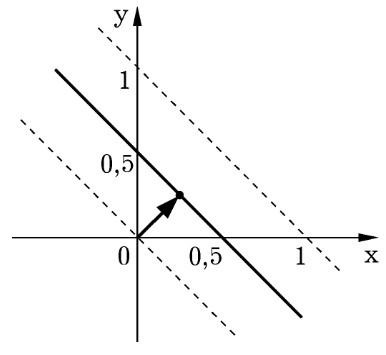
\includegraphics[scale=0.6]{images/module1/question16/1.jpg}
        \caption{}
        \label{fig:picture_16_1}
    \end{figure}

\end{example}


\newpage
\section{
    Матрица перехода от базиса к базису, вывод формулы для преобразования координат вектора при переходе к новому базису. Обратный переход. Работа с тремя и более базисами.
}

% Матрица перехода от базиса к базису
\subsection{
    Матрица перехода от базиса к базису.
}

\begin{definition}
    \textit{\textbf{Матрицей перехода}} от старого базиса к новому называется матрица, элементами \textit{\textbf{столбцов}} которой являются координаты векторов нового базиса, разложенных по старому базису.
    \label{fig:definition_17_1}
\end{definition}

% Вывод формулы для преобразования координат вектора при переходе к новому базису
\subsection{
    Вывод формулы для преобразования координат вектора при переходе к новому базису.
}

Пусть в $n$-мерном линейном пространстве $\mathcal{L}$ заданы два базиса: старый $b = (\vec{b_1}, \ldots, \vec{b_n})$ и новый $c = (\vec{c_1}, \ldots, \vec{c_n})$.

Разложим векторы базиса $c$ по базису $b$:

$$\vec{c_i} = \alpha_{1i}\vec{b_1} + \ldots + \alpha_{ni}\vec{b_n}, \quad i = \overline{1, n}.$$

Запишем эти представления в матричной форме:

$$\vec{c_i} = b \begin{pmatrix} \alpha_{1i} \\ \vdots \\ \alpha_{ni} \end{pmatrix}, \quad  i = \overline{1, n},$$

или

$$c = bT_{b \to c},$$

где

\begin{equation*}
    T_{b \to c} = \left(\begin{array}{ccc}
        \alpha_{11} & \ldots & \alpha_{1n} \\
        \hdotsfor{3} \\
        \alpha_{n1} & \ldots & \alpha_{nn}
    \end{array}\right).
\end{equation*}

% *Полезное дополнение про преобразование координат вектора при переходе от старого базиса к новому
\subsection{
    *Полезное дополнение про преобразование координат вектора при переходе от старого базиса к новому.
    \label{subsection:subsection_17_3}
}

Выберем произвольный вектор $\vec{x} \in \mathcal{L}$ и разложим его в старом базисе $b$:

$$\vec{x} = bx_b, \quad \quad x_b = \begin{pmatrix} x_1 \\ \vdots \\ x_n \end{pmatrix}.$$

Разложение того же вектора в новом базисе $c$ имеет вид:

$$\vec{x} = cx_c, \quad \quad x_c = \begin{pmatrix} x_1' \\ \vdots \\ x_n' \end{pmatrix}.$$

Найдем связь между старыми координатами $x_b$ вектора $\vec{x}$ и его новыми координатами $x_c$. Из соотношений выше следует, что $bx_b = cx_c$. Учитывая, что $c = bT_{b \to c}$, получаем 
$$bx_b = (bT_{b \to c})x_c,$$ или 
$$bx_b = b(T_{b \to c}x_c).$$ 
Последнее равенство можно рассматривать как запись двух разложений одного и того же вектора $\vec{x}$ в базисе $b$. Разложениями соответствуют столбцы координат $x_b$ и $T_{b \to c}x_c$, которые, согласно теореме \ref{thm:theorem_2_3} о единственности разложения вектора по базису, должны быть равны:
$$x_b = T_{b \to c}x_c, \quad \quad \text{или} \quad \quad x_c = T^{-1}_{b \to c}x_b.$$



\newpage


% Обратный переход. Работа с тремя и более базисами
\subsection{
    Обратный переход. Работа с тремя и более базисами.
}

\textbf{Свойства.}

\begin{enumerate}[label={\arabic*°.}]
    \item Матрица перехода невырождена и всегда имеет обратную.
    \begin{proof}~

        Столбцы матрицы перехода - столбцы координат векторов нового \textbf{базиса} в старом. Следовательно, они, как и векторы базиса, линейно независимы. Значит, матрица $T$ невырожденная и имеет обратную матрицу $T^{-1}$.
    \end{proof}
    
    \item Если в $n$-мерном линейном пространстве задан базис $b$, то для любой невырожденной квадратной матрицы $T$ порядка $n$ существует такой базис $c$ в этом линейном пространстве, что $T$ будет матрицей перехода то базиса $b$ к базису $c$.
    \begin{proof}~

        Из невырожденности матрицы $T$ следует, что ее ранг равен $n$, и поэтому ее столбцы, будучи базисными, линейно независимы. Эти столбцы являются столбцами координат векторов системы $c = bT_{b \to c}$. Линейная независимость столбцов матрицы $T$ равносильна линейной независимости системы векторов $c$. Так как система $c$ содержит $n$ векторов, причем линейное пространство $n$-мерно, то согласно теореме $\eqref{thm:theorem_2_1}$, эта система является базисом.
    \end{proof}
    
    \item Если $T_{b \to c}$ - матрица перехода от старого базиса $b$ к новому базису $c$ линейного пространства, то $T^{-1}_{b \to c}$ - матрица перехода от базиса $c$ к базису $b$.
    \begin{proof}~

        Матрица $T_{b \to c}$ невырождена, и поэтому из равенства $c = bT_{b \to c}$ следует, что $cT^{-1}_{b \to c} = b$. Последнее равенство означает, что столбцы матрицы $T^{-1}_{b \to c}$ являются столбцами координат векторов $b$ относительно базиса $c$, т.е. согласно определению $\eqref{fig:definition_17_1}$ $T^{-1}_{b \to c}$ - это матрица перехода от базиса $c$ к базису $b$.
    \end{proof}

    \item Если в линейном пространстве заданы базисы $b, c$ и $d$, причем $T_{b \to c}$ - матрица перехода от базиса $b$ к новому базису $c$, а $T_{c \to d}$ - матрица перехода от базиса $c$ к базису $d$, то произведение этих матриц $T_{b \to c}T_{c \to d}$ - матрица перехода от базиса $b$ к базису $d$.
    \begin{proof}~

        Согласно определению $\eqref{fig:definition_17_1}$ матрицы перехода, имеем равенства
        $$c = bT_{b \to c}, \quad d = cT_{c \to d},$$
        откуда
        $$d = cT_{c \to d} = (b T_{b \to c}) \cdot T_{c \to d} = b(T_{b \to c} \cdot T_{c \to d}),$$
        т.е. $T_{b \to c} \cdot T_{c \to d} = T_{b \to d}$ - матрица перехода от базиса $b$ к базису $d$.
    \end{proof}

    \item Пусть $b_1, b_2, \ldots, b_n$ - это $n$ базисов линейного пространства $\mathcal{V}$ ($n \geq 4$). $T_k$ - матрица перехода от $b_k$ к $b_{k + 1}$, $k = \overline{1, n - 1}$. Тогда матрица перехода от $b_1$ к $b_n$ равна $T_1\cdot T_2 \cdot \ldots \cdot T_{n - 1}$.
    \begin{proof}
        Последовательное применение свойства 4°.
    \end{proof}
\end{enumerate}


\newpage
\section{
    Евклидовы и унитарные пространства. Три примера. Неравенство Коши-Буняковского (Шварца).
}

% Евклидовы и унитарные пространства. Три примера
\subsection{
    Евклидовы и унитарные пространства. Три примера.
}

\textbf{Примеры $\mathcal{E}$:}
\begin{enumerate}
    \item В линейных пространствах $\mathcal{V}_2$ и $\mathcal{V}_3 \colon (\vec{x}, \vec{y}) = |\vec{x}||\vec{y}|\cos \widehat{(\vec{x}, \vec{y})}$.
    \item В арифметическом линейном пространстве $\RR^n \colon (\vec{x}, \vec{y}) = x_1y_1 + \ldots + x_ny_n$. 
    \item Линейное пространство $C[0, 1]$ всех функций, непрерывных на отрезке $[0, 1]$ становится евклидовым, если в нем ввести скалярное произведение:
    $$(\vec{f}, \vec{g}) = \int_{0}^{1} f(x)g(x) \dd x.$$
\end{enumerate}

\textbf{Примеры $\mathcal{U}$:}

\begin{enumerate}
    \item $\CC^n \colon (\vec{x}, \vec{y}) = x_1\overline{y}_1 + x_2\overline{y}_2 + \ldots + x_n\overline{y}_n$.
\end{enumerate}



\newpage


% Неравенство Коши-Буняковского (Шварца)
\subsection{
    Неравенство Коши-Буняковского (Шварца).
}

\begin{theorem}
    Для любых векторов $\vec{x}, \vec{y} \in \mathcal{E}$ (или $\mathcal{U}$) справедливо неравенство Коши-Буняковского
    $$|(\vec{x}, \vec{y})|^2 \leq (\vec{x}, \vec{x}) (\vec{y}, \vec{y}),$$
    причем $|(\vec{x}, \vec{y})|^2 = (\vec{x}, \vec{x}) (\vec{y}, \vec{y}) \iff \vec{x} \parallel \vec{y}.$
\end{theorem}

\begin{corollary}~

    В случае линейного арифметического пр-ва $\RR^n$ неравенство Коши-Буняковского трансформируется в \textbf{неравенство Коши}:
    $$(a_1b_1 + \ldots + a_nb_n)^2 \leq (a_1^2 + \ldots + a_n^2)(b_1^2 + \ldots + b_n^2).$$
    Равенство достигается при линейной зависимости векторов, т.е. $\frac{a_i}{b_i} = const, \quad i = \overline{1, n}$.
\end{corollary}

\begin{corollary}~

    В евклидовом пространстве $C[0, 1]$, скалярное произведение в котором выражается определенным интегралом, неравенство Коши-Буняковского превращается в неравенство Буняковского-Шварца:
    $$\left( \int_0^1 f(x)g(x) \, dx \right)^2 \le \left( \int_0^1 f(x)^2 \, dx \right) \left( \int_0^1 g(x)^2 \, dx \right).$$
\end{corollary}



\newpage


% Неравенство Коши-Буняковского (доказательство для $\mathcal{U}$)
\subsection{
    Неравенство Коши-Буняковского (доказательство для $\mathcal{U}$).
}


\begin{proof}~
    
    При $\vec{y} = \vec{0}$ обе части неравенства равны нулю, значит, неравенство выполняется. Отбрасывая этот очевидный случай, будем считать, что $\vec{y} \ne \vec{0}$. Для любого комплексного числа $t$, в силу аксиомы 4 скалярного произведения, выполняется неравенство 

    $$(\vec{x} + t\vec{y}, \vec{x} + t\vec{y}) \geq 0.$$

    Преобразуем левую часть неравенства, используя аксиомы и свойства скалярного произведения:  
    
    \begin{align*}
        (\vec{x} + t\vec{y}, \vec{x} + t\vec{y}) &= (\vec{x}, \vec{x}) + \underbrace{t(\vec{y}, \vec{x}) + \overline{t}(\vec{x}, \vec{y})}_{\star} + t \cdot \overline{t}(\vec{y}, \vec{y}) = \\
        &= (\vec{x}, \vec{x}) + \underbrace{2 \text{Re}(t(\vec{y}, \vec{x}))}_{\star} + |t|^2(\vec{y}, \vec{y}) = \\
        &= \underbrace{(\vec{y}, \vec{y})}_{\ne 0}|t|^2 + \underbrace{2|(\vec{x}, \vec{y})||t|}_{\star \star} + (\vec{x}, \vec{x}) \geq 0.
    \end{align*}
    
    $\text{\textbf{Примечание} } (\star) \colon$ Пусть $t = p + iq, (\vec{y}, \vec{x}) = a + ib$, $\overline{t} = p - iq, \overline{(\vec{y}, \vec{x})} = a - ib$. Тогда

    \begin{enumerate}
        \item \begin{align*}
            t(\vec{y}, \vec{x}) &+ \overline{t} \cdot (\vec{x}, \vec{y}) = t(\vec{y}, \vec{x}) + \overline{t} \cdot \overline{(\vec{y}, \vec{x})} = \\
            &= (p + iq)(a + ib) + (p - iq)(a - ib) = \\ 
            &= pa + pib + aiq - qb + pa - pib - aiq - qb = 2pa - 2qb = \\
            &= 2 \cdot (pa - qb).
        \end{align*}
        \item \begin{align*}
            2 \cdot \text{Re} (t \cdot (\vec{y}, \vec{x})) &= 2 \cdot \text{Re}((p + iq)(a + ib)) = \\
            &= 2 \cdot \text{Re}(pa - qb + i(pb + aq)) = \\
            &= 2 \cdot (pa - qb).
        \end{align*}
        \item \begin{align*}
            t(\vec{y}, \vec{x}) + \overline{t} \cdot (\vec{x}, \vec{y}) = 2 \cdot \text{Re} (t \cdot (\vec{y}, \vec{x})).
        \end{align*}
    \end{enumerate}

    $\text{\textbf{Примечание} } (\star \star) \colon$ Выберем $t$ так, чтобы $\arg{t} = -\arg{(\vec{y}, \vec{x})}$, тогда $\arg{(\vec{y}, \vec{x})} = -\arg{t}$.

    \begin{gather*}
        t = |t|e^{i\varphi} \\
        \text{Так как }\arg{(\vec{y}, \vec{x})} = -\arg{t}, \text{ то } \\
        (\vec{y}, \vec{x}) = |(\vec{x}, \vec{y})|e^{i(-\varphi)}.
    \end{gather*}

    Итак, 
    
    $$2 \cdot \text{Re} (t \cdot (\vec{y}, \vec{x})) = 2 \cdot \text{Re} (|t|e^{i\varphi} \cdot |(\vec{x}, \vec{y})|e^{-i\varphi}) = 2|t||(\vec{x}, \vec{y})|.$$

    Мы получили квадратным трехчлен относительно параметра $|t|$, неотрицательный при всех действительных значениях параметра. Следовательно, его дискриминант равен нулю или отрицательный, т.е.

    \begin{gather*}
        |(\vec{x}, \vec{y})|^2 - (\vec{x}, \vec{x})(\vec{y}, \vec{y}) \leq 0.
    \end{gather*}
\end{proof}



\newpage


% Неравенство Коши-Буняковского (доказательство для $\mathcal{E}$)
\subsection{
    Неравенство Коши-Буняковского (доказательство для $\mathcal{E}$).
}


\begin{theorem}
    Для любых векторов $\vec{x}, \vec{y}$ евклидова пространства справедливо неравенство Коши-Буняковского

    \begin{equation}
        (\vec{x}, \vec{y})^2 \leq (\vec{x}, \vec{x}) (\vec{y}, \vec{y}).
        \label{equition:equition_18_1}
    \end{equation}
\end{theorem}

\begin{proof}~

    При $\vec{x} = \vec{0}$ обе части неравенства \eqref{equition:equition_18_1} равны нулю согласно свойствам скалярного произведения, значит, неравенство выполняется. Отбрасывая этот очевидный случай, будем считать, что $\vec{x} \ne \vec{0}$. Для любого действительного числа, в силу аксиомы 4 скалярного произведения, выполняется неравенство

    $$(\lambda \vec{x} - \vec{y}, \lambda \vec{x} - \vec{y}) \geq 0.$$

    Преобразуем левую часть неравенства, используя аксиомы и свойства скалярного произведения:

    \begin{align*}
        (\lambda \vec{x} - \vec{y}, \lambda \vec{x} - \vec{y}) &= \lambda (\vec{x}, \lambda \vec{x} - \vec{y}) - (\vec{y}, \lambda\vec{x} - \vec{y}) = \\
        &= \lambda^2\underbrace{(\vec{x}, \vec{x})}_{\ne 0} - 2\lambda(\vec{x}, \vec{y}) + (\vec{y}, \vec{y}) \geq 0.
    \end{align*}

    Мы получили квадратным трехчлен относительно параметра $\lambda$, неотрицательный при всех действительных значениях параметра. Следовательно, его дискриминант равен нулю или отрицательный, т.е.

    $$(\vec{x}, \vec{y})^2 - (\vec{x}, \vec{x})(\vec{y}, \vec{y}) \leq 0.$$
\end{proof}


\newpage
\section{
    Матрица Грама для системы векторов. Определитель и ранг матрицы Грама. Как изменится грамиан, если один из векторов заменить его ортогональной проекцией?
}

% Матрица Грама для системы векторов
\subsection{
    Матрица Грама для системы векторов.
}
    
\begin{definition}
    Пусть даны векторы \( \vec{x}_1, \vec{x}_2, \dots, \vec{x}_m \) в некотором евклидовом пространстве. \textit{\textbf{Матрицей Грама}} этой системы называется квадратная матрица \( \Gamma \) размера \( m \times m \), элементы которой задаются скалярными произведениями:

    \[
    \Gamma = \begin{pmatrix}
    (\vec{x}_1, \vec{x}_1) & (\vec{x}_1, \vec{x}_2) & \cdots & (\vec{x}_1, \vec{x}_m) \\
    (\vec{x}_2, \vec{x}_1) & (\vec{x}_2, \vec{x}_2) & \cdots & (\vec{x}_2, \vec{x}_m) \\
    \vdots     & \vdots     & \ddots & \vdots     \\
    (\vec{x}_m, \vec{x}_1) & (\vec{x}_m, \vec{x}_2) & \cdots & (\vec{x}_m, \vec{x}_m)
    \end{pmatrix},
    \]
    
    где \( (\vec{x}_i, \vec{x}_j) \) обозначает скалярное произведение векторов \( \vec{x}_i \) и \( \vec{x}_j \).
\end{definition}

Её определитель называется определителем Грама (или \textbf{\textit{грамианом}}).

% Определитель и ранг матрицы Грама
\subsection{
    Определитель и ранг матрицы Грама.
}


\begin{itemize}
    \item $\det \Gamma \geq 0$ (всегда неотрицателен).
    \item $\det \Gamma = 0$ $\iff$ векторы $\vec{x}_1, \vec{x}_2, \dots, \vec{x}_m$ линейно зависимы.
    \item Для линейно независимых векторов $\det \Gamma > 0$.
    \item Геометрический смысл: $\det \Gamma$ равен квадрату объёма параллелепипеда, натянутого на векторы.
\end{itemize}

Ранг матрицы Грама равен максимальному числу линейно независимых векторов в системе, т.е. 

$\rank \Gamma(\vec{x}_1, \vec{x}_2, \dots, \vec{x}_m) = \dim \Span (\vec{x}_1, \vec{x}_2, \dots, \vec{x}_m)$.

% Как изменится грамиан, если один из векторов заменить его ортогональной проекцией?
\subsection{
    Как изменится грамиан, если один из векторов заменить его ортогональной проекцией?
}

Рассмотрим линейное пространство $\mathcal{L} = \Span(\vec{e}_1, \ldots, \vec{e}_{k - 1}, \vec{e}_k, \vec{e}_{k + 1}, \ldots, \vec{e}_n)$ и его подпространство 

$\mathcal{H} = \Span(\vec{e}_1, \ldots, \vec{e}_{k - 1}, \vec{e}_{k + 1}, \ldots, \vec{e}_n)$.

\bigbreak

Представим вектор $\vec{e}_k \in \mathcal{L}$ в виде 
$$\vec{e}_k = \vec{e}^{\parallel}_k + \vec{e}^{\perp}_k,$$

где $\vec{e}^{\parallel}_k \in \mathcal{H}$ - ортогональная проекция, а $\vec{e}^{\perp}_k \in \mathcal{H}^\perp$ - ортогональная составляющая.

Значит,

\begin{gather*}
    \vec{e}^{\parallel}_k = \alpha_1\vec{e}_1 + \ldots + \alpha_{k - 1}\vec{e}_{k - 1} + \alpha_{k + 1}\vec{e}_{k + 1} + \ldots + \alpha_n\vec{e}_n. \\
    \downimplies \\
    \vec{e}_1, \ldots, \vec{e}_{k - 1}, \vec{e}^{\parallel}_k, \vec{e}_{k + 1}, \ldots, \vec{e}_n \text{ - линейно зависимы.} \\
    \downimplies \\
    \det \Gamma(\underbrace{\vec{e}_1, \ldots, \vec{e}_{k - 1}, \vec{e}^{\parallel}_k, \vec{e}_{k + 1}, \ldots, \vec{e}_n}_{\text{Система векторов, полученная заменой } \vec{e}_k \text{ на } \vec{e}^{\parallel}_k.}) = 0
\end{gather*}


\newpage
\section{
    Норма вектора в евклидовом пространстве. Привести три примера задания нормы. Свойства нормы (с доказательством).
}

% Норма вектора в евклидовом пространстве
\subsection{
    Норма вектора в евклидовом пространстве.
}

\begin{definition}
    Функция, заданная на линейном пространстве $\mathcal{V}$, которая каждому вектору ставит в соответствие вещественное число, называется \textbf{\textit{нормой}}, если выполнены 3 аксиомы:
    \begin{enumerate}[nosep]
        \item $\norm{\vec{x}} \geq 0$, причем $\norm{\vec{x}} = 0 \iff \vec{x} = 0$;
        \item $\norm{\lambda \vec{x}} = |\lambda| \cdot  \norm{\vec{x}}, \thinspace \lambda \in \RR$;
        \item $\norm{\vec{x} + \vec{y}} \leq \norm{\vec{x}} + \norm{\vec{y}}$ (неравенство треугольника).
    \end{enumerate}
\end{definition}

\begin{theorem}
    Всякое скалярное произведение в евклидовом пространстве определяет норму $\norm{\vec{x}} = \sqrt{(\vec{x}, \vec{x})}$.
\end{theorem}

% Три примера задания нормы
\subsection{
    Три примера задания нормы.
}


\begin{definition}
    Норма вида $\norm{\vec{x}}_2 = \sqrt{(\vec{x}, \vec{x})}$ называется \textbf{\textit{евклидовой}} $(l_2)$
\end{definition}

\begin{definition}
    Норма вида $\norm{\vec{x}}_1 = |x_1| + \dots + |x_n|$ называется \textbf{\textit{октаэдрической}} $(l_1)$
\end{definition}

\begin{definition}
    Норма вида $\norm{\vec{x}}_{\infty} = max\{|x_1|, \dots, |x_n|\}$ называется \textbf{\textit{кубической}} $(l_{\infty})$
\end{definition}

% Свойства нормы
\subsection{
    Свойства нормы.
}

\begin{enumerate}[label={\arabic*°.}]
    \item $\norm{\vec{x}} - \norm{\vec{y}} \leq \norm{\vec{x} \pm \vec{y}} \leq \norm{\vec{x}} + \norm{\vec{y}}$.
    
    \item $\norm{\alpha\vec{x} + \beta\vec{y}} \leq \norm{\alpha\vec{x}} + \norm{\beta\vec{y}} = |\alpha|\norm{\vec{x}} + |\beta|\norm{\vec{y}}$.

    \item $\norm{\vec{x} + \vec{y}}^2 + \norm{\vec{x} - \vec{y}}^2 = 2(\norm{\vec{x}}^2 + \norm{\vec{y}}^2)$.

    \begin{proof}
        \begin{gather*}
            \norm{\vec{x} + \vec{y}}^2 = (\vec{x} + \vec{y}, \vec{x} + \vec{y}) = (\vec{x}, \vec{x}) + (\vec{x}, \vec{y}) + (\vec{y}, \vec{x}) + (\vec{y}, \vec{y}),\\
            \norm{\vec{x} - \vec{y}}^2 = (\vec{x} - \vec{y}, \vec{x} - \vec{y}) = (\vec{x}, \vec{x}) - (\vec{x}, \vec{y}) - (\vec{y}, \vec{x}) + (\vec{y}, \vec{y}),\\
            \norm{\vec{x} + \vec{y}}^2 + \norm{\vec{x} - \vec{y}}^2 = 2(\vec{x}, \vec{x}) + 2(\vec{y}, \vec{y}) = 2(\norm{\vec{x}}^2 + \norm{\vec{y}}^2).
        \end{gather*}
    \end{proof}
    
    \item Если норма порождена скалярным произведением, т.е. $\norm{\vec{z}} = \sqrt{(\vec{z}, \vec{z})}$, то для неё определено
    
    $$(\vec{x}, \vec{y}) = \frac{1}{2}\cdot(\norm{\vec{x} + \vec{y}}^2 - \norm{\vec{x}}^2 - \norm{\vec{y}}^2).$$

    \begin{proof}
        \begin{align*}
            &\frac{1}{2}\cdot(\norm{\vec{x} + \vec{y}}^2 - \norm{\vec{x}}^2 - \norm{\vec{y}}^2) = \\
            &= \frac{1}{2}\cdot((\vec{x} + \vec{y}, \vec{x} + \vec{y}) - (\vec{x}, \vec{x}) - (\vec{y}, \vec{y})) = \\
            &= \frac{1}{2} \cdot ((\vec{x}, \vec{x}) + 2(\vec{x}, \vec{y}) + (\vec{y}, \vec{y})  - (\vec{x}, \vec{x}) - (\vec{y}, \vec{y})) = \\
            &= (\vec{x}, \vec{y}).
        \end{align*}
    \end{proof}
    
    \item В конечномерном пространстве любые две нормы эквивалентны.

    \begin{definition}[P.S.]
        Две нормы $p$ и $q$ на пространстве $\mathcal{V}$ называются эквивалентными, если
        
        $$\exists C_1, C_2 > 0 \colon C_1p(\vec{x}) \leq q(\vec{x}) \leq C_2p(\vec{x}), \forall \vec{x} \in \mathcal{V}.$$
    \end{definition}
\end{enumerate}



\part{Модуль 2.}

    \section{
    Линейный оператор, определение, три 
    примера. Матрица линейного оператора. 
    Вывести формулу для вычисления значений 
    линейного оператора (с помощью его 
    матрицы). Произведение линейных 
    операторов. Матрица для произведения 
    линейных операторов.
 }

% Линейный оператор, определение, три примера
\subsection{
    Линейный оператор, определение, три примера.
}

\begin{definition}
    Пусть $\mathcal{V}, \mathcal{W}$ - 
    линейные пространства над полем $\PP$, 
    $\dim \mathcal{V} = n, \dim \mathcal{W} = m$. 
    Отображение $\mathscr{A} \colon \mathcal{V} 
    \to \mathcal{W}$ называется 
    \textit{\textbf{линейным оператором}}, 
    если $\forall \vec{x}, \vec{y} \in 
    \mathcal{V}$ и $\forall \lambda \in \PP$ 
    выполнены следующие условия:
    
    \begin{enumerate}[nosep]
        \item $\mathscr{A}(\vec{x} + \vec{y}) = 
        \mathscr{A}(\vec{x}) + \mathscr{A}(\vec{y}),$
        \item $\mathscr{A}(\alpha\vec{x}) = 
        \alpha\mathscr{A}(\vec{x})$,
    \end{enumerate}
    где $\vec{x}$ - прообраз $\vec{y} = \mathscr{A}\vec{x}$,
    $\vec{y} = \mathscr{A}\vec{x}$ - образ $\vec{x}$.
\end{definition}

\begin{example}~

    \begin{enumerate}[nosep]
        \item Нулевой: $\zeroperator\vec{x} = \vec{0}$.
        \item Тождественный/единичный: 
        $\identityoperator\vec{x} = \vec{x}$.
        \item Оператор дифференцирования $\mathscr{D} \colon P_n(x) \to P_n(x)$, действующий по правилу $\mathscr{D}f = f'$.
    \end{enumerate}
\end{example}



\newpage


% Матрица линейного оператора
\subsection{
    Матрица линейного оператора.
}

Пусть $\mathcal{V}$ и $\mathcal{W}$ - два линейных пространства.

Пусть $e = (\vec{e_1}, \ldots, \vec{e_n})$ - некоторый базис в $\mathcal{V}$, $f = (\vec{f_1}, \ldots, \vec{f_m})$ - некоторый базис в $\mathcal{W}$. 

Тогда $\mathscr{A}\vec{e_1}, \ldots, \mathscr{A}\vec{e_n}$ - это некоторые векторы в $\mathcal{W}$; значит, их можно, причем единственным образом, разложить по базису $\vec{f_1}, \ldots, \vec{f_m}$:

$$\mathscr{A}\vec{e_1} = a_{11}\vec{f_1} + \ldots + a_{m1}\vec{f_m}$$
$$\ldots \ldots \ldots \ldots \ldots \ldots \ldots \ldots \ldots$$
$$\mathscr{A}\vec{e_n} = a_{1n}\vec{f_1} + \ldots + a_{mn}\vec{f_m},$$

где $(a_{ij} \in \PP)$.

\begin{definition}
    Матрицу, составленную из координатных столбцов векторов $\mathscr{A}\vec{e_1}, \ldots, \mathscr{A}\vec{e_n}$ в базисе $f = (\vec{f_1}, \ldots, \vec{f_m})$, называют \textit{\textbf{матрицей линейного оператора}} $\mathscr{A}$ в базисе $f$.
\end{definition}



\newpage

% Вывести формулу для вычисления значений линейного оператора (с помощью его матрицы)
\subsection{
    Вывести формулу для вычисления значений линейного оператора (с помощью его матрицы).
}

\begin{theorem}
    Пусть $\mathscr{A} \colon \mathcal{L} \to \mathcal{L}$ - линейный оператор. Тогда столбец $y_b$ координат вектора $\vec{y} = \mathscr{A}\vec{x}$ в данном базисе $b$ линейного пространства $\mathcal{L}$ равен произведению $A_bx_b$ матрицы $A_b$ оператора $\mathscr{A}$ в базисе $b$ на столбец $x_b$ координат вектора $\vec{x}$ в том же базисе: $y_b = A_bx_b$.
    \label{thm:theorem_21_1}
\end{theorem}

\begin{proof}
    Выберем произвольный вектор $\vec{x} = x_1\vec{b_1} + \ldots + x_n\vec{b_n}$. Его образом будет вектор

    \begin{align*}
        \vec{y} &= \mathscr{A}\vec{x} =  \mathscr{A}(x_1\vec{b_1} + \ldots + x_n\vec{b_n}) = x_1(\mathscr{A}\vec{b_1}) + \ldots + x_n(\mathscr{A}\vec{b_n}) = \\
        &= x_1(a_{11}\vec{b_1} + \ldots + a_{n1}\vec{b_n}) + \ldots + x_n(a_{1n}\vec{b_1} + \ldots + a_{nn}\vec{b_n}) = \\
        &= (a_{11}x_1 + \ldots + a_{1n}x_n)\vec{b_1} + \ldots + (a_{n1}x_1 + \ldots + a_{nn}x_n)\vec{b_n} = \\
        &= \begin{pmatrix}
            \vec{b}_1 & \ldots & \vec{b}_n
        \end{pmatrix} \cdot \begin{pmatrix} 
            a_{11}x_1 + \ldots + a_{1n}x_n \\
            \vdots \\
            a_{n1}x_1 + \ldots + a_{nn}x_n
        \end{pmatrix}
    \end{align*}

    Столбец координат вектора $\vec{y} = \mathscr{A}\vec{x}$ в базисе $b$ имеет вид

    \begin{equation*}
        y_b = (\mathscr{A}\vec{x})_b = \begin{pmatrix} 
            a_{11}x_1 + \ldots + a_{1n}x_n \\
            \vdots \\
            a_{n1}x_1 + \ldots + a_{nn}x_n
        \end{pmatrix} =
        \begin{pmatrix} 
            a_{11} \thinspace \thinspace \ldots \thinspace \thinspace a_{1n} \\
            \ldots \ldots \ldots \\
            a_{n1} \thinspace \thinspace \ldots \thinspace \thinspace a_{nn}
        \end{pmatrix}
        \begin{pmatrix} 
            x_1 \\
            \vdots \\
            x_n
        \end{pmatrix} = A_bx_b
    .\end{equation*}
\end{proof}

\begin{corollary}
    $\vec{y} = \mathscr{A}\vec{x} = bA_bx_b.$
\end{corollary}



\newpage


% Произведение линейных операторов. Матрица для произведения линейных операторов
\subsection{
    Произведение линейных операторов. Матрица для произведения линейных операторов.
}

\begin{definition}
    \textbf{\textit{Произведением операторов}} $\mathscr{A} \colon \mathcal{V} \to \mathcal{W}$ и $\mathscr{B} \colon \mathcal{L} \to \mathcal{V}$ называется оператор $(\mathscr{A}\mathscr{B}) \colon \mathcal{L} \to \mathcal{W}$, действующий по правилу $(\mathscr{A}\mathscr{B})\vec{x} = \mathscr{A}(\mathscr{B}\vec{x}), \forall \vec{x} \in \mathcal{L}$. 
    
    Этот оператор является линейным, так как $\forall \vec{x}, \vec{y} \in \mathcal{L},\thinspace \thinspace \forall \lambda, \mu \in \RR$:

    $$(\mathscr{A}\mathscr{B})(\lambda\vec{x} + \mu\vec{y}) = \mathscr{A}(\mathscr{B}(\lambda\vec{x} + \mu\vec{y})) = \mathscr{A}(\lambda\mathscr{B}\vec{x} + \mu\mathscr{B}\vec{y}) = \lambda\mathscr{A}(\mathscr{B}\vec{x}) + \mu\mathscr{A}(\mathscr{B}\vec{y}) = \lambda(\mathscr{A}\mathscr{B})\vec{x} + \mu(\mathscr{A}\mathscr{B})\vec{y}.$$
\end{definition}

\begin{theorem}
    Пусть в линейном пространстве $\mathcal{L}$ действуют линейные операторы $\mathscr{A}$ и $\mathscr{B}$, а $A_b$ и $B_b$ - матрицы этих линейных операторов в некотором базисе $b$. Тогда матрицей линейного оператора $\mathscr{B}\mathscr{A}$ в том же базисе $b$ является матрица $B_bA_b$.
\end{theorem}

\begin{proof}
    $\vec{y} = (\mathscr{B}\mathscr{A})\vec{x} = \mathscr{B}(\mathscr{A}\vec{x}) = \mathscr{B}(bA_bx_b) = b(B_b(A_bx_b)) = b(B_bA_b)x_b.$
\end{proof}


\newpage
\section{
    Линейный оператор, определение, три примера. Преобразование матрицы линейного оператора при переходе к новому базису (вывести формулу).
 }

% Преобразование матрицы линейного оператора при переходе к новому базису (вывести формулу)
\subsection{
    Преобразование матрицы линейного оператора при переходе к новому базису (вывести формулу).
}

\begin{theorem}
    Матрицы $A_b$ и $A_e$ линейного оператора $\mathscr{A} \colon \mathcal{L} \to \mathcal{L}$, записанные в базисах $b$ и $e$ линейного пространства $\mathcal{L}$, связаны друг с другом соотношением
    
    $$A_e = T^{-1}_{b \to e}A_bT_{b \to e}.$$
\end{theorem}

\begin{proof}~

    Пусть $\vec{y} = \mathscr{A}\vec{x}$. Обозначим координаты векторов $\vec{x}$ и $\vec{y}$ в старом базисе $b$ через $x_b$ и $y_b$, а в новом базисе $e$ - через $x_e$ и $y_e$. Поскольку действие линейного оператора $\mathscr{A}$ в матричной форме в базисе $b$ имеет вид $y_b = A_bx_b$ (\textbf{*}см. теорему \ref{thm:theorem_21_1}), а координаты векторов $\vec{x}$ и $\vec{y}$ в новом и старом базисах связаны между собой равенствами (\textbf{*}см. билет 17.)

    $$x_b = T_{b \to e}x_e, \quad \quad y_b = T_{b \to e}y_e,$$

    то получаем

    $$y_e = T^{-1}_{b \to e}y_b = T^{-1}_{b \to e}(A_bx_b) = T^{-1}_{b \to e}(A_bT_{b \to e}x_e) = (T^{-1}_{b \to e}A_bT_{b \to e})x_e.$$
    Равенство $y_e = (T^{-1}_{b \to e}A_bT_{b \to e})x_e$ является матричной формой записи действия линейного оператора $\mathscr{A}$ в базисе $e$ и поэтому, согласно теореме \ref{thm:theorem_21_1}, $T^{-1}_{b \to e}A_bT_{b \to e} = A_e$. 

    Изложенное доказательство теоремы хорошо иллюстрирует следующая диаграмма:

    \begin{figure}[H]
        \centering
        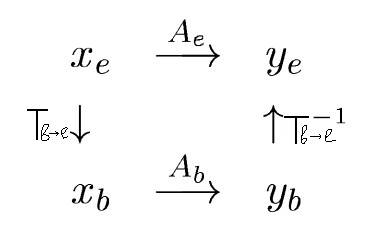
\includegraphics[scale=0.5]{images/module2/question22/1.jpg}
        \label{fig:picture_22_1}
    \end{figure}
\end{proof}


\newpage
\section{
    Линейный оператор, определение, три примера. Ранг и дефект, ядро и образ линейного оператора. Теорема про размерности. Инвариантное подпространство линейного оператора.  
}

% Ранг и дефект, ядро и образ линейного оператора
\subsection{
    Ранг и дефект, ядро и образ линейного оператора.
}

Пусть $\mathscr{A} \colon \mathcal{V} \to \mathcal{W}$ - линейный оператор.

\begin{definition}
    \textbf{\textit{Образом}} оператора $\mathscr{A}$ называется множество всех векторов $\vec{y} \in \mathcal{W}$, представимых в виде $\vec{y} = \mathscr{A}\vec{x}$.
\end{definition}

\begin{designation}
    $\Im \mathscr{A}$.
\end{designation}

\begin{definition}
    \textbf{\textit{Ядром}} оператора $\mathscr{A}$ называется множество всех векторов $\vec{x} \in \mathcal{V} \colon \mathscr{A}\vec{x} = \vec{0}_{\mathcal{W}}$.
\end{definition}

\begin{designation}
    $\ker \mathscr{A}$.
\end{designation}

\begin{definition}
    Размерность образа линейного оператора $\mathscr{A}$ называется \textbf{\textit{рангом}} линейного оператора $\mathscr{A}$. 
\end{definition}

\begin{designation}
    $\rank \mathscr{A}$.
\end{designation}

\begin{definition}
    Размерность ядра линейного оператора $\mathscr{A}$ называется \textbf{\textit{дефектом}} линейного оператора $\mathscr{A}$. 
\end{definition}

\begin{designation}
    $\defect \mathscr{A}$.
\end{designation}



\newpage


% Теорема про размерности
\subsection{
    Теорема про размерности.
}

\begin{theorem}
    Пусть $\mathscr{A} \colon \mathcal{V} \to \mathcal{W}$ - линейный оператор, $\dim \mathcal{V} = n$. Тогда $\defect \mathscr{A} + \rank \mathscr{A} = \dim \mathcal{V}$.
\end{theorem}

\begin{proof}~

    Пусть $\vec{e}_1, \ldots, \vec{e}_r$ - базис в $\ker \mathscr{A}$. Дополним его до базиса $\vec{e}_1, \ldots, \vec{e}_r, \vec{e}_{r + 1}, \ldots, \vec{e}_n$ всего пространства $\mathcal{V}$. Докажем, что $\dim \Im \mathscr{A} = n - r$. Для этого рассмотрим набор векторов $\mathscr{A}(\vec{e}_{r + 1}), \ldots, \mathscr{A}(\vec{e}_n)$ и докажем, что он является базисом в $\Im \mathscr{A}$.

    \bigbreak

    $\Im \mathscr{A} = \Span(\underbrace{\mathscr{A}(\vec{e}_1), \ldots, \mathscr{A}(\vec{e}_r)}_{\vec{0}}, \mathscr{A}(\vec{e}_{r + 1}), \ldots, \mathscr{A}(\vec{e}_n)) = \Span(\mathscr{A}(\vec{e}_{r + 1}), \ldots, \mathscr{A}(\vec{e}_n))$.

    Предположим, что $\lambda_{r + 1}\mathscr{A}(\vec{e}_{r + 1}) + \ldots + \lambda_n\mathscr{A}(\vec{e}_n) = \mathscr{A}(\lambda_{r + 1}\vec{e}_{r + 1} + \ldots + \lambda_n\vec{e}_n) = \vec{0}_{\mathcal{W}}.$

    Значит, $\lambda_{r + 1}\vec{e}_{r + 1} + \ldots + \lambda_n\vec{e}_n \in \ker \mathscr{A}$, но тогда $\lambda_{r + 1}\vec{e}_{r + 1} + \ldots + \lambda_n\vec{e}_n = \mu_1\vec{e}_1 + \ldots + \mu_r\vec{e}_r$, для некоторых $\mu_1, \ldots, \mu_r$. Так как векторы $\vec{e}_1, \ldots, \vec{e}_n$ - линейно независимы, то все $\lambda_i = 0$ (и $\mu_j$ тоже), следовательно, векторы $\vec{e}_{r + 1}, \ldots, \vec{e}_n$ - линейно независимы.

    \bigbreak

    При этом любой вектор $\vec{y} \in \Im \mathscr{A}$ является линейной комбинацией векторов $\mathscr{A}(\vec{e}_{r + 1}), \ldots, \mathscr{A}(\vec{e}_n)$.

    \bigbreak

    Следовательно, $\mathscr{A}(\vec{e}_{r + 1}), \ldots, \mathscr{A}(\vec{e}_n)$ - базис в $\Im \mathscr{A} \Rightarrow \dim \Im \mathscr{A} = n - r$.

    \bigbreak

    Значит, $\dim \ker \mathscr{A} + \dim \Im \mathscr{A} = \defect \mathscr{A} + \rank \mathscr{A} = r + n - r = n = \dim \mathcal{V}$.
\end{proof}

\bigbreak

\begin{comment}
    Можно ли утверждать, что если $\mathscr{A} \colon \mathcal{V} \to \mathcal{V}$, то $\Im \mathscr{A} + \ker \mathscr{A} = \mathcal{V}$?

    \bigbreak

    \textbf{Ответ:} нельзя. 
    
    Например, $\mathscr{D} \colon p \longmapsto p'$.

    $p \in P_n(x)$

    $\Im \mathscr{D} = P_{n - 1}(x)$
    
    $\ker \mathscr{D} = P_0(x)$

    Но $P_0(x) + P_{n - 1}(x) \ne P_n(x)$.
    
\end{comment}



\newpage


% Инвариантное подпространство линейного оператора
\subsection{
    Инвариантное подпространство линейного оператора.
}

\begin{definition}
    Пусть $\mathscr{A} \colon \mathcal{L} \to \mathcal{L}$ - линейный оператор. Подпространство $\mathcal{V} \in \mathcal{L}$ называется \textbf{\textit{инвариантным подпространством}} оператора $\mathscr{A}$, если оператор $\mathscr{A}$ отображает всякий вектор $\vec{x} \in \mathcal{V}$, в вектор, также принадлежащий подпространству $\mathcal{V}$, то есть $\forall \vec{x} \in \mathcal{V} \colon \vec{y} = \mathscr{A}\vec{x} \in \mathcal{V}$.
\end{definition}

\begin{example}~

    \begin{itemize}
        \item Тривиальными примерами являются: само пространство $\mathcal{L}$ и нулевое подпространство (состоящее из единственного нулевого вектора).
        \item Любой собственный вектор оператора порождает его одномерное инвариантное подпространство.
        \item Ядро линейного оператора $\ker \mathcal{L}$. 
    \end{itemize}
\end{example}


\newpage
\section{
    Операции с линейными операторами. Ранг произведения операторов. Линейное пространство линейных операторов.
}

% Операции с линейными операторами
\subsection{
    Операции с линейными операторами.
}

\begin{definition}
    Операторы $\mathscr{A} \colon \mathcal{V} \to \mathcal{W}$ и $\mathscr{B} \colon \mathcal{V} \to \mathcal{W}$ называются \textbf{\textit{равными}}, если $\mathscr{A}\vec{x} = \mathscr{B}\vec{x}, \forall \vec{x} \in \mathcal{V}$.
\end{definition}

\begin{definition}
    \textbf{\textit{Суммой операторов}} $\mathscr{A} \colon \mathcal{V} \to \mathcal{W}$ и $\mathscr{B} \colon \mathcal{V} \to \mathcal{W}$ называется оператор $(\mathscr{A} + \mathscr{B}) \colon \mathcal{V} \to \mathcal{W}$, действующий по правилу $(\mathscr{A} + \mathscr{B})\vec{x} = \mathscr{A}\vec{x} + \mathscr{B}\vec{x}, \forall \vec{x} \in \mathcal{V}$.
\end{definition}

\begin{definition}
    \textbf{\textit{Произведением оператора}} $\mathscr{A} \colon \mathcal{V} \to \mathcal{W}$ \textbf{\textit{на действительное число}} $\lambda$ называется оператор $(\lambda\mathscr{A}) \colon \mathcal{V} \to \mathcal{W}$, действующий по правилу $(\lambda\mathscr{A})\vec{x} = \lambda(\mathscr{A}\vec{x}), \forall \vec{x} \in \mathcal{V}$.
\end{definition}

\begin{definition}
    \textbf{\textit{Произведением операторов}} $\mathscr{A} \colon \mathcal{V} \to \mathcal{W}$ и $\mathscr{B} \colon \mathcal{L} \to \mathcal{V}$ называется оператор $(\mathscr{A}\mathscr{B}) \colon \mathcal{L} \to \mathcal{W}$, действующий по правилу $(\mathscr{A}\mathscr{B})\vec{x} = \mathscr{A}(\mathscr{B}\vec{x}), \forall \vec{x} \in \mathcal{L}$.
\end{definition}



\newpage


% Ранг произведения операторов
\subsection{
    Ранг произведения операторов.
}

Для любых двух линейных операторов $\mathscr{A}$ и $\mathscr{B}$, действующих в линейном пространстве $\mathcal{L}$, выполняется соотношение

$$\rank(\mathscr{A}\mathscr{B}) \leq \min\{\rank\mathscr{A}, \rank\mathscr{B}\}$$

\begin{proof}~

    Рассмотрим оператор $\mathscr{A}$ как линейный оператор $\mathscr{A}\colon \Im\mathscr{B} \to \mathcal{L}$. Размерность образа оператора не превосходит размерности линейного пространства, из которого он действует, так как сумма и дефекта и ранга совпадает с размерностью этого пространства.

    $$\rank(\mathscr{A}\mathscr{B}) = \dim \Im (\mathscr{A}\mathscr{B}) \leq \dim \Im \mathscr{B} = \rank \mathscr{B}.$$
    
    Так как образ линейного оператора $\mathscr{A}\mathscr{B}$ является линейным подпространством образа линейного оператора $\mathscr{A}$, то
    
    $$\rank(\mathscr{A}\mathscr{B}) \leq \rank \mathscr{A}.$$
\end{proof}


\begin{comment}~

    Доказанное соотношение можно перенести на квадратные матрицы. 
    
    Получаем, 
    $$\rank{(AB)} \leq \min\{\rank A, \rank B\}.$$

    Пусть $B$ - невырожденная. То есть ее ранг равен размерности матрицы. 
    
    Тогда $\rank{(AB)} \leq \rank A$ и одновременно $\rank A = \rank ((AB)B^{-1}) \leq \rank (AB)$.

    То есть 
    
    $$\rank (AB) \leq \rank A \leq \rank (AB).$$
    
    Следовательно, при умножении матрицы $A$ справа на невырожденную матрицу ее ранг не изменяется. 
    
    При умножении матрицы $A$ слева на невырожденную матрицу ранг также не изменяется, что доказывается аналогично.
    \label{comment:comment_24_2}
\end{comment}



\newpage


% Линейное пространство линейных операторов
\subsection{
    Линейное пространство линейных операторов.
}

\begin{definition}
    Линейное пространство $\mathcal{L}(\mathcal{V}, \mathcal{W})$ линейных операторов из линейного пространства $\mathcal{V}$ в линейное пространство $\mathcal{W}$ называют \textbf{\textit{линейным пространством линейных операторов}}.
\end{definition}

\begin{proof}[Проверка на линейность пространства $\mathcal{L}$]~

    Пусть даны линейные операторы $\mathscr{A}б \mathscr{B} \in \mathcal{L}(\mathcal{V}, \mathcal{W})$. 

    Поскольку
    \begin{align*}
        (\mathscr{A} + &\mathscr{B})(\alpha\vec{x} + \beta \vec{y}) = \mathscr{A}(\alpha\vec{x} + \beta \vec{y}) + \mathscr{B}(\alpha\vec{x} + \beta \vec{y}) = \\
        &= (\alpha\mathscr{A}\vec{x} + \beta\mathscr{A}\vec{y}) + (\alpha\mathscr{B}\vec{x} + \beta\mathscr{B}\vec{y}) = \\
        &= \alpha(\mathscr{A}\vec{x} + \mathscr{B}\vec{x}) + \beta(\mathscr{A}\vec{y} + \mathscr{B}\vec{y}) = \\
        &= \alpha(\mathscr{A} + \mathscr{B})\vec{x} + \beta(\mathscr{A} + \mathscr{B})\vec{y}
    \end{align*}

    и

    \begin{align*}
        (\lambda\mathscr{A})&(\alpha\vec{x} + \beta \vec{y}) = \lambda(\mathscr{A}(\alpha\vec{x} + \beta\vec{y})) = \lambda (\mathscr{A}(\alpha\vec{x}) + \mathscr{A}(\beta\vec{y})) = \\ 
        &= (\alpha \lambda)\mathscr{A}\vec{x} + (\beta \lambda)\mathscr{A}\vec{y} = \alpha(\lambda \mathscr{A}\vec{x}) + \beta(\lambda \mathscr{A}\vec{y}) = \\
        &= \alpha((\lambda\mathscr{A})\vec{x}) + \beta((\lambda\mathscr{A})\vec{y})
    \end{align*}

    отображения $\mathscr{A} + \mathscr{B}$ и $\lambda \mathscr{A}$ действительно являются линейными операторами. Таким образом, относительно введенных нами операций множество $\mathcal{L}(\mathcal{V}, \mathcal{W})$ замкнуто. Проверив аксиомы линейного пространства, можно убедиться, что $\mathcal{L}(\mathcal{V}, \mathcal{W})$ относительно этих операций является линейным пространством.
\end{proof}


\newpage
\section{
    Собственные векторы и собственные значения линейного оператора. Характеристическое уравнение и характеристический многочлен линейного оператора. Нахождение собственных значений линейного оператора (вывести характеристическое уравнение). Геометрическая и алгебраическая кратность. Жорданова нормальная форма.
}

% Собственные векторы и собственные значения линейного оператора
\subsection{
    Собственные векторы и собственные значения линейного оператора.
}

\begin{definition}
    Ненулевой вектор $\vec{x}$ в линейном пространстве $\mathcal{L}$ называют \textbf{\textit{собственным вектором}} линейного оператора $\mathscr{A}\colon \mathcal{L} \to \mathcal{L}$, если для некоторого действительного числа $\lambda$ выполняется соотношение $\mathscr{A}\vec{x} = \lambda\vec{x}$. При этом число $\lambda$ называют \textbf{\textit{собственным значением}} линейного оператора $\mathscr{A}$.
\end{definition}

% Характеристическое уравнение и характеристический многочлен линейного оператора
\subsection{
    Характеристическое уравнение и характеристический многочлен линейного оператора.
}

Для произвольной квадратной матрицы $A = (a_{ij})$ порядка $n$ рассмотрим определитель

$$\det(A - \lambda E) = \begin{vmatrix} 
    a_{11} - \lambda & a_{12} & \ldots & a_{1n} \\
    a_{21} & a_{22} - \lambda & \ldots & a_{2n} \\
    \vdots & \vdots & \ddots & \vdots \ \\
    a_{n1} & a_{12} & \ldots & a_{nn} - \lambda \\
\end{vmatrix},$$

где $E$ - единичная матрица, а $\lambda$ - действительное переменное.

\begin{definition}
    Многочлен $\chi_A(\lambda) = \det(A - \lambda E)$ называют \textbf{\textit{характеристическим многочленом}} матрицы $A$, а уравнение $\chi_A(\lambda) = 0$ — \textbf{\textit{характеристическим уравнением}} матрицы $A$.
\end{definition}

\begin{definition}
    \textbf{\textit{Характеристическим многочленом линейного оператора}} $\mathscr{A} \colon \mathcal{L} \to \mathcal{L}$ называют характеристический многочлен его матрицы $A$, записанной в некотором базисе, а \textbf{\textit{характеристическим уравнением}} этого \textbf{\textit{оператора}} - характеристическое уравнение матрицы $A$.
\end{definition}

% *Полезные факты, которые тоже могут быть на экзамене
\subsection{
    *Полезные факты, которые тоже могут быть на экзамене.
}

\begin{definition}
    Квадратные матрицы $A$ и $B$ порядка $n$ называются \textit{\textbf{подобными}}, если существует такая невырожденная матрица $P$, что $P^{-1}AP = B$.
    \label{def:definition_17_1}
\end{definition}

\begin{theorem}
    Если матрицы $A$ и $B$ подобны, то $\det A = \det B$.
    \label{thm:theorem_25_1}
\end{theorem}

\begin{proof}~

    Если матрицы подобны, то согласно определению \eqref{def:definition_17_1}, существует такая невырожденная матрица $P$, что $B = P^{-1}AP$. Так как определитель произведения квадратных матриц равен произведению определителей этих матриц, а $\det(P^{-1}) = (\det P)^{-1}$, то получаем
    $$\det B = \det(P^{-1}AP) = \det(P^{-1})\det A \det P = \det(P)^{-1}\det A \det P = \det A.$$
\end{proof}

\begin{corollary}
    Определитель матрицы линейного оператора не зависит от выбора базиса.
\end{corollary}

\begin{proof}
    Действительно, возьмем матрицы $A_b$ и $A_e$ линейного оператора $\mathscr{A}$ в двух различных базисах $b$ и $e$.

    $$A_e = T^{-1}_{b \to e}A_bT_{b \to e}.$$

    Согласно определению \eqref{def:definition_17_1}, матрицы $A_b$ и $A_e$ подобны. Поэтому $\det A_b = \det A_e$ по теореме \ref{thm:theorem_25_1}.
\end{proof}



\newpage


% Нахождение собственных значений линейного оператора (вывести характеристическое уравнение)
\subsection{
    Нахождение собственных значений линейного оператора (вывести характеристическое уравнение).
}

\begin{theorem}
    Для того чтобы действительное число $\lambda$ являлось собственным значением линейного оператора, необходимо и достаточно, чтобы оно было корнем характеристического уравнения этого оператора.
\end{theorem}

\begin{proof}~
    \begin{description}
        \item[$(\implies)$] 
            Пусть число $\lambda$ является собственным значением линейного оператора $\mathscr{A} \colon \mathcal{L} \to \mathcal{L}$. Это значит, что существует вектор $\vec{x} \ne \vec{0}$, для которого 

            $$\mathscr{A}\vec{x} = \lambda \vec{x}.$$

            Используя тождественный оператор $\mathscr{I}\vec{x} = \vec{x}$, преобразуем равенство: $\mathscr{A}\vec{x} = \lambda\mathscr{I}\vec{x}$, или
            
            $$(\mathscr{A} - \lambda\mathscr{I})\vec{x} = \vec{0}.$$

            Запишем векторное равенство выше в каком-либо базисе $b$. Матрицей линейного оператора $\mathscr{A} - \lambda\mathscr{I}$ будет матрица $A - \lambda E$, где $A$ - матрица линейного оператора $\mathscr{A}$ в базисе $b$, а $E$ - единичная матрица, и пусть $x$ - столбец координат собственного вектора $\vec{x}$. Тогда $x \ne 0$, а векторное равентсво выше равносильно матричному

            $$(A - \lambda E) = 0,$$

            которое представляет собой матричную форму записи ОСЛАУ с квадратной матрицей $A - \lambda E$ порядка $n$. Эта система имеет ненулевое решение, являющееся столбцом координат $x$ собственного вектора $\vec{x}$. Поэтому $\det(A - \lambda E) = 0$. А это означает, что $\lambda$ является корнем характеристического уравнения линейного оператора $\mathscr{A}$.
        \item[$(\impliedby)$]
            Приведенные рассуждения можно привести в обратном порядке. Если $\lambda$ является корнем характеристического уравнения, то в заданном базисе $b$ выполняется равенство $\det (A - \lambda E) = 0$. Следовательно, матрица ОСЛАУ, записанной в матричной форме, вырождена, и система имеет ненулевое решение $x$. Это ненулевое решение $x$ представляет собой набор координат в базисе $b$ некоторого ненулевого вектора $\vec{x}$, для которого выполняется равенство $(\mathscr{A} - \lambda\mathscr{I})\vec{x} = \vec{0}$. Значит, число $\lambda$ - собственное значение линейного оператора $\mathscr{A}$.
    \end{description}
\end{proof}



\newpage


% Геометрическая и алгебраическая кратность
\subsection{
    Геометрическая и алгебраическая кратность.
}

\begin{definition}
    \textbf{\textit{Геометрической кратностью}} собственного значения линейного оператора называется максимальное число линейно независимых собственных векторов, соответствующих данному собственному значению.
\end{definition}

\begin{definition}
    \textbf{\textit{Алгебраической кратностью}} собственного значения линейного оператора называется его кратность как корня характеристического многочлена.
\end{definition}



\newpage


% Жорданова нормальная форма
\subsection{
    Жорданова нормальная форма.
}

Для произвольного действительного числа $\mu$ введем обозначение матрицы порядка $s$:

$$J_s(\mu) = \begin{pmatrix} 
    \mu & 1 & 0 & \ldots & 0 & 0 \\
    0 & \mu & 1 & \ldots & 0 & 0 \\
    \hdotsfor6 \\
    0 & 0 & 0 & \ldots & \mu & 1 \\
    0 & 0 & 0 & \ldots & 0 & \mu
\end{pmatrix}$$

Для любого комплексного числа $\lambda = \alpha + i\beta (\beta \ne 0)$ введем обозначение блочной матрицы порядка $2r$:

$$C_r(\alpha, \beta) = \begin{pmatrix} 
    C(\alpha, \beta) & E & 0 & \ldots & 0 & 0 \\
    0 & C(\alpha, \beta) & E & \ldots & 0 & 0 \\
    \hdotsfor6 \\
    0 & 0 & 0 & \ldots & C(\alpha, \beta) & E \\
    0 & 0 & 0 & \ldots & 0 & C(\alpha, \beta)
\end{pmatrix},$$

где $C(\alpha, \beta) = \begin{pmatrix} 
    \alpha & \beta \\
    -\beta & \alpha
\end{pmatrix}$. Все остальные блоки также являются квадратными матрицами порядка 2, где $E$ - единичная матрица, 0 - нулевая.

Блочно-диагональную матрицу вида

\[
A = \begin{pmatrix}
    C_{r_1}(\alpha_1, \beta_1) &        &        &        &  \\
                               & \ddots &        &        & \scaleobj{4}{0}   \\
                               &        & C_{r_m}(\alpha_m, \beta_m) &        &   \\
                               &        &        & J_{s_1}(\mu_1) &   \\
                               & \scaleobj{4}{0} &        &     & \ddots  &  \\
                               &        &        &        & &J_{s_k}(\mu_k)
\end{pmatrix},
\]

где $\alpha_j, \beta_j (j = \overline{1, m})$ и $\mu_l (l = \overline{1, k})$ - действительные числа, называют \textbf{\textit{жордановой}}, ее диагональные блоки - \textbf{\textit{жордановыми клетками}}. Жорданову матрицу $A'$, подобную данной матрице $A$, называют \textbf{\textit{жордановой нормальной формой}} матрицы $A$.


\newpage
\section{
    Формулировка теоремы Гамильтона – Кэли. След линейного оператора. Инварианты.
}

% Формулировка теоремы Гамильтона – Кэли
\subsection{
    Формулировка теоремы Гамильтона – Кэли.
}

Квадратную матрицу можно использовать в качестве значения переменного в произвольном многочлене. Тогда значением многочлена от матрицы будет матрица того же порядка, что и исходная. Интерес представляют такие многочлены, значение которых от данной матрицы есть нулевая матрица. Их называют аннулирующими многочленами. Оказывается, что одним из таких аннулирующих многочленов для матрицы является ее характеристический многочлен.

\begin{theorem}
    Для любой квадратной матрицы характеристический многочлен является ее аннулирующим многочленом.
\end{theorem}

% След линейного оператора
\subsection{
    След линейного оператора.
}

\begin{definition}
    \textbf{\textit{Следом линейного оператора $\mathscr{A}$ (матрицы $A$)}} называется сумма диагональных элементов матрицы $A$ линейного оператора $\mathscr{A}$.
\end{definition}

\begin{designation}
    $\tr \mathscr{A}$ или $\Sp \mathscr{A}$.
\end{designation}

% Инварианты
\subsection{
    Инварианты.
}

Коэффициенты характеристического многочлена не зависят от выбора базиса (если представить в виде $\sum_{k=0}^{n} d_k \lambda^k
$), т.е. являются инвариантами относительно выбора базиса.

\begin{comment}
    Наиболее просто выражается коэффициент $d_{n - 1} = \tr \mathscr{A}$.
\end{comment}

\begin{comment}
    Коэффициент $d_0$ характеристического многочлена совпадает со значением этого многочлена при $\lambda = 0$ и равен определителю линейного оператора $\mathscr{A}$.
\end{comment}


\newpage
\section{
    Формулировка теоремы про ЖНФ. Алгоритм построения ЖНФ. Определение количества клеток. Нахождение базиса. 
}

\begin{theorem}
    Пусть $\lambda_1, \lambda_2, \ldots$ – все собственные числа (корни характеристического уравнения) оператора $\mathscr{A}$, действующего в $n$-мерном пространстве $\mathcal{L}$. Тогда в $\mathcal{L}$ существует базис, в котором матрица оператора имеет блочно-диагональный вид $A_J = J_1 \oplus J_2 \oplus \ldots \oplus J_s$, т.е. является прямой суммой жордановых клеток (блоков), каждая из которых является квадратной матрицей, на главной диагонали которой стоят одинаковые числа $\lambda_i$, над диагональю стоят единицы, а все остальные элементы равны нулю:

    \begin{figure}[H]
        \centering
        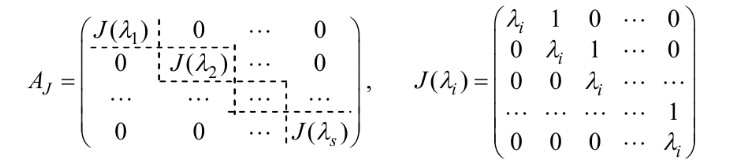
\includegraphics[scale=0.7]{images/module2/question27/1.jpg}
        \label{fig:picture_27_1}
    \end{figure} 
\end{theorem}


\newpage
\section{
    Собственные векторы и собственные значения линейного оператора. Доказать независимость характеристического многочлена и характеристического уравнения линейного оператора от выбора базиса.
}

\begin{theorem}
    Характеристические многочлены (уравнения) подобных матриц совпадают.
    \label{thm:theorem_28_1}
\end{theorem}

\begin{proof}~

    Пусть квадратные матрицы $A$ и $A'$ одного порядка подобны, т.е. существует такая невырожденная матрица $P$ того же порядка, что $A' = P^{-1}AP$. Тогда в силу свойств определителей имеем

    \begin{align*}
        \chi_{A'}&(\lambda) = \det(A' - \lambda E) = \det(P^{-1}AP - \lambda P^{-1}EP) = \\
        &=\det(P^{-1}(A - \lambda E)P) = \det P^{-1}\det(A - \lambda E)\det P = \\
        &=\det(A - \lambda E) = \chi_A(\lambda).
    \end{align*}
\end{proof}

\begin{theorem}
    Характеристический многочлен и характеристическое уравнение линейного оператора не зависят от выбора базиса.
\end{theorem}

\begin{proof} Пусть 

    \begin{enumerate}[nosep]
        \item $\mathscr{A} \colon \mathcal{L} \to \mathcal{L}$ - линейный оператор,
        \item $A_b$ - матрица линейного оператора $\mathscr{A}$ в некотором ''старом'' базисе $b$, 
        \item $A_e$ - матрица линейного оператора $\mathscr{A}$  в некотором ''новом'' базисе $e$.
    \end{enumerate}
    
    Тогда 
    
    $$A_e = T^{-1}_{b \to e}A_bT_{b \to e},$$ где $T_{b \to e}$ - матрица перехода от базиса $b$ к базису $e$.

    $A_e$ и $A_b$ - две подобные матрицы.

    Значит, по теореме \ref{thm:theorem_28_1} характеристические многочлены двух подобных матриц $A_e$ и $A_b$ равны. Следовательно, и характеристический многочлен линейного оператора не зависит от выбора базиса.
\end{proof}


\newpage
\section{
    Собственные векторы и собственные значения линейного оператора. Свойство собственных векторов линейного оператора, соответствующих одному и тому же собственному значению (с доказательством).
}

% Свойство собственных векторов линейного оператора, соответствующих одному и тому же собственному значению (с доказательством)
\subsection{
    Свойство собственных векторов линейного оператора, соответствующих одному и тому же собственному значению (с доказательством).
}

Если $\vec{x}$ - собственный вектор оператора $\mathscr{A}$, отвечающий собственному значению, то для любого числа $k \ne 0$ вектор $k\vec{x}$ также является собственным вектором оператора $\mathscr{A}$, отвечающим собственному значению.

\begin{proof}~

    $\mathscr{A}\vec{x} = \lambda\vec{x}$,
    
    $\mathscr{A}(k\vec{x}) = k\mathscr{A}\vec{x} = k\lambda\vec{x}$.
\end{proof}

Если $\vec{x}$ и $\vec{y}$ - собственные векторы оператора $\mathscr{A}$, отвечающие собственному значению, то вектор $\vec{x} + \vec{y} \ne \vec{0}$ также является собственным вектором, отвечающим собственному значению.

\begin{proof}~

    $\mathscr{A}\vec{x} = \lambda\vec{x}$,
    
    $\mathscr{A}\vec{y} = \lambda\vec{y}$,
    
    $\mathscr{A}(\vec{x} + \vec{y}) = \mathscr{A}\vec{x} + \mathscr{A}\vec{y} = \lambda\vec{x} + \lambda\vec{y} = \lambda(\vec{x} + \vec{y})$.
\end{proof}

\begin{corollary}[свойство]~

    Множество всех собственных векторов, отвечающих данному собственному значению, с добавлением $\vec{0}$ является линейным подпространством для данного пространства $\mathcal{L}$. Такое подпространство называется \textbf{\textit{собственным подпространством $\mathcal{L}$}}.
\end{corollary}


\newpage
\section{
    Собственные векторы и собственные значения линейного оператора. Свойство собственных векторов линейного оператора, соответствующих различным собственным значениям (с доказательством).
}

% Свойство собственных векторов линейного оператора, соответствующих различным собственным значениям (с доказательством)
\subsection{
    Свойство собственных векторов линейного оператора, соответствующих различным собственным значениям (с доказательством).
}

\begin{theorem}
    Пусть собственные значения $\lambda_1, \ldots, \lambda_r$ линейного оператора $\mathscr{A}$ попарно различны. Тогда система соответствующих им собственных векторов $\vec{e}_1, \ldots, \vec{e}_r$ линейно независима.
\end{theorem}

\begin{proof}~

    Воспользуемся методом математической индукции.

    При $r = 1$ утверждение теоремы верно, так как линейная независимость системы из одного вектора означает, что этот вектор ненулевой, а собственный вектор, согласно его определению, является ненулевым.

    Пусть утверждение верно при $r = m$, т.е. для произвольной системы из $m$ собственных векторов $\vec{e}_1, \ldots, \vec{e}_m$. Добавим к системе векторов еще один собственный вектор $\vec{e}_{m + 1}$, отвечающий собственному значению $\lambda_{m + 1}$, и докажем, что расширенная таким способом система векторов останется линейно независимой. Рассмотрим произвольную линейную комбинацию полученной системы векторов и предположим, что она равна нулевому вектору:

    \begin{equation}
        \alpha_1\vec{e}_1 + \ldots + \alpha_m\vec{e}_m + \alpha_{m + 1}\vec{e}_{m + 1} = \vec{0}.
        \label{eq:equation_30_1}
    \end{equation}

    $$\alpha_1\mathscr{A}\vec{e}_1 + \ldots + \alpha_m\mathscr{A}\vec{e}_m + \alpha_{m + 1}\mathscr{A}\vec{e}_{m + 1} = \vec{0}.$$

    \begin{equation}
        \alpha_1\lambda_1\vec{e}_1 + \ldots + \alpha_m\lambda_m\vec{e}_m + \alpha_{m + 1}\lambda_{m + 1}\vec{e}_{m + 1} = \vec{0}.
        \label{eq:equation_30_2}
    \end{equation}

    Умножим равенство \eqref{eq:equation_30_1} на $\lambda_{m + 1}$ и вычтем из него равенство \eqref{eq:equation_30_2}

    $$\alpha_1(\lambda_1 - \lambda_{m + 1})\vec{e}_1 + \ldots + \alpha_m(\lambda_m - \lambda_{m + 1})\vec{e}_m = \vec{0}.$$

    Так как система векторов $\vec{e}_1, \ldots, \vec{e}_m$ по предположению, линейно независима, то у полученной линейной комбинации все коэффициенты равны нулю:

    \begin{equation}
        \alpha_k(\lambda_k - \lambda_{m + 1}) = 0, k = \overline{1, m}.
        \label{eq:equation_30_3}
    \end{equation}

    Поскольку все собственные значения $\lambda_i$ попарно различны, то из равенств \eqref{eq:equation_30_3} следует, что $\alpha_1 = \alpha_2 = \ldots = \alpha_m = 0$. Значит, соотношение \eqref{eq:equation_30_1} можно записать в виде $\alpha_{m + 1}\vec{e}_{m + 1} = \vec{0}$, а так как вектор $\vec{e}_{m + 1}$ ненулевой (как собственный вектор), то $\alpha_{m + 1} = 0$. В итоге получаем, что равенство \eqref{eq:equation_30_1} выполняется лишь в случае тривиальной линейной комбинации. Тем самым мы доказали, что система векторов $\vec{e}_1, \ldots, \vec{e}_m, \vec{e}_{m + 1}$ линейно независима.
\end{proof}


\newpage
\section{
    Дать определение сопряженного и самосопряженного линейного оператора. Доказать, что все корни характеристического многочлена самосопряженного оператора вещественны.
}

% Дать определение сопряженного и самосопряженного линейного оператора
\subsection{
    Дать определение сопряженного и самосопряженного линейного оператора.
}

Пусть $\mathcal{E}$ - евклидово пространство.

\begin{definition}
    Линейный оператор $\mathscr{A^*} \colon \mathcal{E} \to \mathcal{E}$ называют сопряженным к линейному оператору $\mathscr{A} \colon \mathcal{E} \to \mathcal{E}$, если для любых векторов $\vec{x}, \vec{y} \in \mathcal{E}$ верно равенство
    $$(\mathscr{A}\vec{x}, \vec{y}) = (\vec{x}, \mathscr{A^*}\vec{y}).$$
\end{definition}

\begin{example}~
    
    Вектор $\vec{a} \in \mathcal{V}_3$ порождает линейный оператор $\mathscr{A} \colon \mathcal{V}_3 \to \mathcal{V}_3$ согласно формуле
    
    $$\mathscr{A}\vec{x} = \vec{a} \times \vec{x}.$$

    Найдем оператор, сопряженный оператору $\mathscr{A}$:
    \begin{align*}
        (\mathscr{A}\vec{x}, &\vec{y}) = (\vec{a} \times \vec{x}, \vec{y}) = \vec{a}\vec{x}\vec{y} = \vec{y}\vec{a}\vec{x} = (\vec{y} \times \vec{a}, \vec{x}) = \\
        &= (\vec{x}, \vec{y} \times \vec{a}) = (\vec{x}, -\vec{a} \times \vec{y}) = (\vec{x}, -\mathscr{A}\vec{y}).
    \end{align*}

    Значит, $\mathscr{A^*} = -\mathscr{A}.$
\end{example}

\begin{definition}
    Линейный оператор $\mathscr{A}$, действующий в евклидовом пространстве, называют самосопряженным, если $\mathscr{A^*} = \mathscr{A}$. То есть для любых векторов $\vec{x}$ и $\vec{y}$ верно равенство

    $$(\mathscr{A}\vec{x}, \vec{y}) = (\vec{x}, \mathscr{A}\vec{y}).$$
\end{definition}

\begin{example}
    Тождественный $\mathscr{I}$ и нулевой $\mathscr{O}$.
\end{example}



\newpage


% Доказать, что все корни характеристического многочлена самосопряженного оператора вещественны
\subsection{
    Доказать, что все корни характеристического многочлена самосопряженного оператора вещественны.
}

\begin{theorem}
    Матрица самосопряженного оператора в любом ортонормированном базисе является симметрической.
\end{theorem}

\begin{theorem}
    Все корни характеристического многочлена самосопряженного оператора вещественны.
\end{theorem}

\begin{proof}~

    Будем доказывать, что все корни характеристического уравнения симметрической матрицы действительны.

    Предположим, что $\lambda \in \CC$ является корнем характеристического уравнения симметрической матрицы, т.е. $\det (A - \lambda E) = 0$. Тогда СЛАУ $(A - \lambda E)x = 0$ имеет некоторое ненулевое решение $x = \begin{pmatrix} x_1 & \cdots & x_n \end{pmatrix} ^ T$, состоящее из комплексных чисел $x_k, k = \overline{1, n}$. Рассмотрим столбец $\overline{x}$, комплексно сопряженный к столбцу $x$. Умножим равенство $(A - \lambda E)x = 0$ слева на строку $\overline{x}^T$. Тогда

    $$\overline{x}^T(A - \lambda E)x = 0,$$

    или

    $$\overline{x}^TAx = \lambda \overline{x}^Tx.$$

    Так как произведение комплексного числа на сопряженное к нему является действительным числом, равным квадрату модуля комплексного числа, а $x$ - ненулевое решение, то
    
    $$\overline{x}^Tx = \overline{x}_1x_1 + \ldots + \overline{x}_nx_n = |x_1|^2 + \ldots + |x_n|^2 > 0,$$
    То есть матричное произведение $\overline{x}^Tx$ - действительное положительное число.

    $$\lambda = \frac{\overline{x}^TAx}{\overline{x}^Tx},$$

    причем знаменатель дроби справа является действительным числом. Следовательно, число $\lambda$ будет действительным, если числитель этой дроби $w = \overline{x}^TAx$ будет действительным.

    В силу симметричности матрицы $A$

    $$w = w^T = (\overline{x}^TAx)^T = x^TA^T\overline{x} = x^TA\overline{x}.$$

    С учетом свойств операции комплексного сопряжения матриц и благодаря тому, что элементами матрицы $A$ являются действительные числа, получаем

    $$\overline{w} = \overline{\overline{x}^TAx} = (\overline{\overline{x}})^T\overline{A}\overline{x} = x^TA\overline{x} = w.$$

    Комплексное число, самосопряженное себе - это действительное число. Следовательно, и $w$ является действительным.
\end{proof}


\newpage
\section{
    Дать определение самосопряженного линейного  оператора. Свойство собственных векторов самосопряженного линейного оператора, отвечающих различным собственным значениям (с доказательством).
}

% Свойство собственных векторов самосопряженного линейного оператора, отвечающих различным собственным значениям (с доказательством)
\subsection{
    Свойство собственных векторов самосопряженного линейного оператора, отвечающих различным собственным значениям (с доказательством).
}

\begin{theorem}
    Собственные векторы самосопряженного оператора, отвечающие различным собственным значениям, ортогональны.
\end{theorem}

\begin{proof}~

    Рассмотрим самосопряженный оператор $\mathscr{A}$ и два его собственных вектора $\vec{x}_1$ и $\vec{x}_2$, отвечающие различным собственным значениям $\lambda_1$ и $\lambda_2$. Тогда $\mathscr{A}\vec{x}_1 = \lambda_1\vec{x}_1$ и $\mathscr{A}\vec{x}_2 = \lambda_2\vec{x}_2$. Поэтому

    \begin{equation}
        (\mathscr{A}\vec{x}_1, \vec{x}_2) = (\lambda_1\vec{x}_1, \vec{x}_2) = \lambda_1(\vec{x}_1, \vec{x}_2).
        \label{eq:equation_32_1}
    \end{equation}

    Но так как $\mathscr{A}$ является самосопряженным оператором, то $(\mathscr{A}\vec{x}_1, \vec{x}_2) = (\vec{x}_1, \mathscr{A}\vec{x}_2)$. Значит,

    \begin{equation}
        (\mathscr{A}\vec{x}_1, \vec{x}_2) = (\vec{x}_1, \mathscr{A}\vec{x_2}) = (\vec{x}_1, \lambda_2\vec{x}_2) = \lambda_2(\vec{x}_1, \vec{x}_2).
        \label{eq:equation_32_2}
    \end{equation}

    Приравнивая правые части соотношений \eqref{eq:equation_32_1} и \eqref{eq:equation_32_2}, получаем

    $$\lambda_1(\vec{x}_1, \vec{x}_2) = \lambda_2(\vec{x}_1, \vec{x}_2),$$

    или

    $$(\lambda_1 - \lambda_2)(\vec{x}_1, \vec{x}_2) = 0.$$

    Так как $\lambda_1 \ne \lambda_2$, $(\vec{x}_1, \vec{x}_2) = 0$, что и означает ортогональность векторов $\vec{x}_1$ и $\vec{x}_2$.
\end{proof}


\newpage
\section{
    Ортогональные матрицы и их свойства.
}

\begin{definition}
    Квадратную матрицу $O$ называют \textbf{\textit{ортогональной}}, если она удовлетворяет условию

    \begin{equation}
        O^TO = E,
        \label{eq:equation_33_1}
    \end{equation}

    где $E$ — единичная матрица.
\end{definition}

\begin{example}
    Простейший пример - единичная матрица $E$, так как $E^TE = EE = E$.
\end{example}

\begin{example}
    $U = \begin{pmatrix}
    \cos \varphi & -\sin \varphi \\
    \sin \varphi & \cos \varphi
    \end{pmatrix}$.
\end{example}

\subsection*{Свойства ортогональных матриц.}

Пусть $O$ - ортогональная матрица.

\begin{enumerate}[label={\arabic*°.}]
    \item $\det O = \pm 1$.
    
    \begin{proof}~
    
        $\det(O^TO) = \det O^T \det O = (\det O)^2$.
        
        Так как $\det E = 1$, то и $(\det O)^2 = 1$. Следовательно, $\det O = \pm 1$.
    \end{proof}
    
    \item $O^{-1} = O^T$.

    \begin{proof}~
    
        Согласно свойству 1, ортогональная матрица невырождена и поэтому имеет обратную $O^{-1}$. Умножая равенство \eqref{eq:equation_33_1} справа на $O^{-1}$, получаем

        $$(O^TO)O^{-1} = EO^{-1},$$

        откуда $O^T(OO^{-1}) = O^{-1}$. Но $OO^{-1} = E$, поэтому $O^T = O^{-1}$.
    \end{proof}

    \item $OO^T = E$.

    \begin{proof}
        Согласно свойству 2 и определению обратной матрицы, $OO^T = OO^{-1} = E$.
    \end{proof}

    \item $O^T$ - тоже ортогональная.

    \begin{proof}~
    
        Нужно для произвольной ортогональной матрицы $O$ доказать равенство

        $$(O^T)^TO^T = E,$$

        представляющее собой запись соотношения \eqref{eq:equation_33_1} для предполагаемой ортогональной матрицы $O^T$ (\textbf{*}вместо $O$). Так как, согласно свойству операции транспонирования, $(O^T)^T = O$, равенство выше эквивалентно $OO^T = E$, которое верно в силу свойства 3.
    \end{proof}

    \item Произведение двух ортогональных матриц $O$ и $Q$ одного порядка является ортогональной матрицей.

    \begin{proof}
        Для доказательства достаточно проверить выполнение равенства \eqref{eq:equation_33_1} для матрицы $OQ$:

        $$(OQ)^T(OQ) = (Q^TO^T)OQ = Q^T(O^TO)Q = Q^TEQ = Q^TQ = E.$$
    \end{proof}

    \item $O^{-1}$ - тоже ортогональная.

    \begin{proof}~
    
        Согласно свойству 1, ортогональная матрица вырождена, а потому имеет обратную. Согласно свойству 2, матрица, обратная к ортогональной, совпадает с транспонированной. Наконец, согласно свойству 4, матрица, транспонированная к ортогональной, является ортогональной.
    \end{proof}
\end{enumerate}


\newpage
\section{
    Ортогональное преобразование евклидова пространства. Свойства ортогональных преобразований (с доказательством).
}

% Ортогональное преобразование евклидова пространства
\subsection{
    Ортогональное преобразование евклидова пространства.
}

Пусть $\mathcal{E}$ - евклидово пространство, $\mathscr{A} \colon \mathcal{E} \to \mathcal{E}$ - некоторый линейный оператор.

\begin{definition}
     Говорят, что $\mathscr{A}$ задает \textbf{\textit{ортогональное преобразование (называется ортогональным оператором)}}, если $\forall \vec{x}, \vec{y} \in \mathcal{V} \colon (\mathscr{A}\vec{x}, \mathscr{A}\vec{y}) = (\vec{x}, \vec{y})$.
\end{definition}

% Свойства ортогональных преобразований
\subsection{
    Свойства ортогональных преобразований.
}

\begin{enumerate}[label={\arabic*°.}]
    \item Сохраняет ортогональность, т.е. $\vec{x} \perp \vec{y} \Rightarrow \mathscr{A}\vec{x} \perp \mathscr{A}\vec{y}$.

    \begin{proof}
        Очевидно.
    \end{proof}
    
    \item Сохраняет норму вектора, т.е. $\norm{\mathscr{A}\vec{x}} = \norm{\vec{x}}$.

    \begin{proof}
        $\norm{\mathscr{A}\vec{x}} = \sqrt{(\mathscr{A}\vec{x}, \mathscr{A}\vec{x})} = \sqrt{(\vec{x}, \vec{x})} = \norm{\vec{x}}$.
    \end{proof}

    \item Сохраняет углы между ненулевыми векторами.

    \begin{proof}
        $\widehat{(\mathscr{A}\vec{x}, \mathscr{A}\vec{y})} = \arccos \frac{(\mathscr{A}\vec{x}, \mathscr{A}\vec{y})}{\norm{\mathscr{A}\vec{x}}\cdot\norm{\mathscr{A}\vec{y}}} = \arccos \frac{(\vec{x}, \vec{y})}{\norm{\vec{x}}\cdot\norm{\vec{y}}} = \widehat{(\vec{x}, \vec{y})}$.
    \end{proof}

    \item Пусть $\mathscr{A} \colon \mathcal{E} \to \mathcal{E}$ - ортогональный оператор, $\vec{e}_1, \ldots, \vec{e}_n$ - ОНБ в $\mathcal{E}$. Тогда $\mathscr{A}\vec{e}_1, \ldots, \mathscr{A}\vec{e}_n$ - ОНБ в $\mathcal{E}$.

    \begin{proof}~
    
        $(\mathscr{A}\vec{e}_i, \mathscr{A}\vec{e}_j) = (\vec{e}_i, \vec{e}_j) = \delta_{ij} \text{ (символ Кронекера)}$.

        $\norm{\mathscr{A}\vec{e}_i} = 1$; $\mathscr{A}\vec{e}_1, \ldots, \mathscr{A}\vec{e}_n$ попарно ортогональны, а значит, ЛНЗ. К тому же, $\dim \mathcal{E} = n$, а $\mathscr{A}\vec{e}_1, \ldots, \mathscr{A}\vec{e}_n$ - тоже $n$. Значит, $\mathscr{A}\vec{e}_1, \ldots, \mathscr{A}\vec{e}_n$ - ОНБ.
    \end{proof}

    \item Пусть 
    
    \begin{itemize}
        \item $\mathcal{E}$ - $n$-мерное евклидово пространство;
        \item $\vec{e}_1, \ldots, \vec{e}_n$ - некоторый ОНБ $\mathcal{E}$;
        \item $\mathscr{A} \colon \mathcal{E} \to \mathcal{E}$ - некоторый линейный оператор.
        \item $\mathscr{A}\vec{e}_1, \ldots, \mathscr{A}\vec{e}_n$ - тоже ОНБ $\mathcal{E}$.
    \end{itemize}

    Тогда $\mathscr{A}$ - ортогональный оператор.

    \begin{proof}~
    
        Требуется доказать, что

        $$\forall \vec{x}, \vec{y} \in \mathcal{E} \colon (\mathscr{A}\vec{x}, \mathscr{A}\vec{y}) = (\vec{x}, \vec{y}).$$

        Возьмем произвольные $\vec{x}, \vec{y} \in \mathcal{E}$.

        Разложим по базису $\vec{e}_1, \ldots, \vec{e}_n$:

        \begin{gather*}
            \vec{x} = x_1\vec{e}_1 + \ldots + x_n\vec{e}_n \\
            \vec{y} = y_1\vec{e}_1 + \ldots + y_n\vec{e}_n
        \end{gather*}

        Найдем:

        \begin{align*}
            (\mathscr{A}\vec{x}, \mathscr{A}\vec{y}) &= (\mathscr{A}(x_1\vec{e}_1 + \ldots + x_n\vec{e}_n), \mathscr{A}(y_1\vec{e}_1 + \ldots + y_n\vec{e}_n)) = \\
            &= (x_1\cdot\mathscr{A}\vec{e}_1 + \ldots + x_n\cdot\mathscr{A}\vec{e}_n, y_1\cdot\mathscr{A}\vec{e}_1 + \ldots + y_n\cdot\mathscr{A}\vec{e}_n) = \\
            &= \left\{ 
            \begin{array}{l}
                \text{Получилось, что} \\
                \text{у вектора } \mathscr{A}\vec{x} \\
                \text{в базисе } \mathscr{A}\vec{e}_1, \ldots, \mathscr{A}\vec{e}_n \\
                \text{координаты } \begin{pmatrix}
                    x_1 \\
                    \vdots \\
                    x_n
                \end{pmatrix}; \\
                \text{у вектора } \vec{y} \text{ аналогично}.
            \end{array} \right\} \underbrace{=}_{\text{Следствие } \ref{corollary:corollary_1}} \\
            &\underbrace{=}_{\text{Следствие } \ref{corollary:corollary_1}} x_1y_1 + \ldots + x_ny_n = (\vec{x}, \vec{y}).
        \end{align*}
    \end{proof}

    \item Пусть 
    
    \begin{itemize}
        \item $\mathcal{E}$ - $n$-мерное евклидово пространство;
        \item $\vec{e}_1, \ldots, \vec{e}_n$ - некоторый ОНБ $\mathcal{E}$;
        \item $\mathscr{A} \colon \mathcal{E} \to \mathcal{E}$ - ортогональный оператор.
    \end{itemize}

    Тогда матрица $A_e$ линейного оператора $\mathscr{A}$ в базисе $\vec{e}_1, \ldots, \vec{e}_n$ - ортогональная.

    \begin{proof}~
    
        \begin{align*}
            (\mathscr{A}\vec{x}, \mathscr{A}\vec{y}) &\underbrace{=}_{\text{Лемма } \ref{lemma:lemma_1}} (\mathscr{A}\vec{x})^T_e\cdot\Gamma_e\cdot(\mathscr{A}\vec{y})_e = \\
            &= (A_e\vec{x}_e)^T\cdot\Gamma_e\cdot(A_e\vec{y}_e) = \\
            &= \vec{x}^T\cdot A^T_e\Gamma_eA_e\vec{y}_e.
        \end{align*}

        При этом

        $$(\vec{x}, \vec{y}) = \vec{x}^T_e\cdot\Gamma_e\cdot\vec{y}_e.$$

        Из этого ясно, что 
        $$A^T_e\Gamma_eA_e = \Gamma_e.$$

        Так как $e$ - ОНБ, то $\Gamma_e = E \in \RR^{n \times n}$.

        И тогда $A^T_e \cdot A_e = E$.
    \end{proof}

    \item Справедлив и обратный факт свойству 6:

    Если линейный оператор $\mathscr{A} \colon \mathcal{E} \to \mathcal{E}$ в ОНБ $\vec{e}_1, \ldots, \vec{e}_n$ имеет ортогональную матрицу, то $\mathscr{A}$ задает ортогональное преобразование.

    \begin{proof}~
    
        Действительно, 

        \begin{align*}
            (\mathscr{A}\vec{x}, \mathscr{A}\vec{y}) &\underbrace{=}_{\text{Лемма } \ref{lemma:lemma_1}} (\mathscr{A}\vec{x})^T_e\cdot\Gamma_e\cdot(\mathscr{A}\vec{y})_e = \\
            &= (A_e\vec{x}_e)^T\cdot E\cdot(A_e\vec{y}_e) = \\
            &= \vec{x}^T\cdot \underbrace{A^T_eA_e}_{ E}\vec{y}_e = \\
            &= \vec{x}^T\vec{y}_e = \\
            &= (\vec{x}, \vec{y}).
        \end{align*}
    \end{proof}
\end{enumerate}


\newpage
\section{
    Дать определение квадратичной формы. Матрица квадратичной формы и ее преобразование при переходе к новому базису (вывести формулу).
}

\begin{definition}
    \textbf{\textit{Квадратичной формой}} называется сумма вида $$f(x_1, \ldots, x_n) = \sum_{i=1}^n b_{ii}x_i^2 + \sum_{1 \leq i < j \leq n} 2b_{ij}x_ix_j,$$

    где $b_{ij}$ - заданные числа, $1 \leq i < j < n$.
\end{definition}

Ясно, что

$$
f(x_1, x_2, \ldots, x_n) = 
\begin{pmatrix}
x_1 & x_2 & \cdots & x_n
\end{pmatrix}
\begin{pmatrix}
    b_{11} & b_{12} & \cdots & b_{1n} \\
    b_{21} & b_{22} & \cdots & b_{2n} \\
    \vdots & \vdots & \ddots & \vdots \\
    b_{n1} & b_{n2} & \cdots & b_{nn}
\end{pmatrix}
\begin{pmatrix}
    x_1 \\
    x_2 \\
    \vdots \\
    x_n
\end{pmatrix}.
$$

Столбец $\begin{pmatrix}
    x_1 \\
    x_2 \\
    \vdots \\
    x_n
\end{pmatrix}$ можно рассматривать как координаты вектора $\vec{x}$ в некотором 'первичном' базисе $\vec{e}_1, \vec{e}_2, \ldots, \vec{e}_n$, а полученную матрицу $\begin{pmatrix}
    b_{11} & b_{12} & \cdots & b_{1n} \\
    b_{21} & b_{22} & \cdots & b_{2n} \\
    \vdots & \vdots & \ddots & \vdots \\
    b_{n1} & b_{n2} & \cdots & b_{nn}
\end{pmatrix}$ - как матрицу квадратичной формы в этом 'первичном' базисе $\vec{e}_1, \vec{e}_2, \ldots, \vec{e}_n$. 

Как она изменится при переходе к новому базису?

Мы знаем, что если $\begin{pmatrix}
    x_1 \\
    x_2 \\
    \vdots \\
    x_n
\end{pmatrix}$ - координаты вектора $\vec{x}$ в базисе $e$, а $\begin{pmatrix}
    y_1 \\
    y_2 \\
    \vdots \\
    y_n
\end{pmatrix}$ - координаты того же вектора $\vec{x}$ в базисе $f$, то

$$\begin{pmatrix}
    x_1 \\
    x_2 \\
    \vdots \\
    x_n
\end{pmatrix} = T_{e \to f}\begin{pmatrix}
    y_1 \\
    y_2 \\
    \vdots \\
    y_n
\end{pmatrix}\text{ (см. \ref{subsection:subsection_17_3}).}$$

Тогда 

$$\begin{pmatrix}
x_1 & x_2 & \cdots & x_n
\end{pmatrix} = \left(T_{e \to f}\begin{pmatrix}
    y_1 \\
    y_2 \\
    \vdots \\
    y_n
\end{pmatrix}\right)^T = \begin{pmatrix}
y_1 & y_2 & \cdots & y_n
\end{pmatrix} \cdot T_{e \to f}^T.$$

Значит,

$$
f(x_1, x_2, \ldots, x_n) = 
\begin{pmatrix}
y_1 & y_2 & \cdots & y_n
\end{pmatrix}
\underbrace{
T_{e \to f}^T
\begin{pmatrix}
    b_{11} & b_{12} & \cdots & b_{1n} \\
    b_{21} & b_{22} & \cdots & b_{2n} \\
    \vdots & \vdots & \ddots & \vdots \\
    b_{n1} & b_{n2} & \cdots & b_{nn}
\end{pmatrix}
T_{e \to f}}_{\text{матрица кв. формы в новом базисе.}}
\begin{pmatrix}
    y_1 \\
    y_2 \\
    \vdots \\
    y_n
\end{pmatrix}.
$$

Значит,

$$\underbracket{B_f}_{\mathclap{\substack{\text{матр. кв.} \\ \text{формы} \\ \text{в новом} \\ \text{базисе } f.}}} = T_{e \to f}^T\underbracket{B_e}_{\mathclap{\substack{\text{исх. матр.} \\ \text{кв. формы} \\ \text{(в старом} \\ \text{базисе } e).}}}T_{e \to f}.$$


\newpage
\section{
    Ранг квадратичной формы, его независимость от выбора базиса. Закон инерции квадратичных форм (с доказательством). 
}

% Ранг квадратичной формы, его независимость от выбора базиса
\subsection{
    Ранг квадратичной формы, его независимость от выбора базиса.
}

\begin{definition}
    Ранг матрицы $A$ квадратичной формы называют \textbf{\textit{рангом квадратичной формы}}.
\end{definition}

При изменении базиса линейного пространства матрица $A$ квадратичной формы преобразуется по формуле $A' = U^TAU$, где $U$ - матрица перехода. Матрица $U$, как матрица перехода, является невырожденной, поэтому ранг $A'$ совпадает с рангом $A$, так как при умножении на невырожденную матрицу ранг не меняется. (см. замечание \ref{comment:comment_24_2}). 

То есть ранг квадратичной формы не зависит от выбора базиса.



\newpage


% Закон инерции квадратичных форм
\subsection{
    Закон инерции квадратичных форм (с доказательством).
}

\begin{theorem} Пусть
    \begin{enumerate}
        \item $\mathcal{V}$ - $n$-мерное линейное пространство.
        \item $\mathscr{B}: \mathcal{V} \times \mathcal{V} \to \RR$ - симметрическая билинейная форма.
        \item $\text{КФ}(\vec{x}) = \mathscr{B}(\vec{x}, \vec{x})$ - соответствующий ей функционал, который может быть записан в виде различных квадратичных форм в зависимости от базиса.
    \end{enumerate}

    Тогда как бы мы ни выбирали канонический базис, количество положительных, количество отрицательных коэффициентов и количество нулевых коэффициентов в каноническом виде КФ будут всегда одними и теми же.
\end{theorem}

\begin{proof}~

    Пусть $\vec{f}_1, \ldots, \vec{f}_n$ и $\vec{g}_1, \ldots, \vec{g}_n$ - два канонических базиса, причем в первом базисе 

    $$\vec{x} = \sum_{k = 1}^{n}x_k\vec{f}_k \text{ и КФ}(\vec{x}) = \sum_{k = 1}^{n}\lambda_kx^2_k.$$

    а во втором базисе

    $$\vec{x} = \sum_{k = 1}^{n}y_k\vec{g}_k \text{ и КФ}(\vec{x}) = \sum_{k = 1}^{n}\mu_ky^2_k.$$

    Будем считать, что:

    \begin{enumerate}
        \item Среди $\lambda_1, \ldots, \lambda_n$ первые $p$ положительные, а остальные $\leq 0$.
        \item Среди $\mu_1, \ldots, \mu_n$ первые $s$ положительные, а остальные $\leq 0$.
    \end{enumerate}

    Отделим положительные слагаемые

    $$\sum_{k = 1}^{p}\underbrace{\lambda_k}_{> 0}x^2_k + \sum_{k = p + 1}^{n}\underbrace{\lambda_k}_{\leq 0}x^2_k = \sum_{k = 1}^{s}\underbrace{\mu_k}_{> 0}y^2_k + \sum_{k = s + 1}^{n}\underbrace{\mu_k}_{\leq 0}y^2_k.$$

    Заметим, что любая из этих сумм может оказаться пустой.

    Перенесем

    \begin{equation}
        \sum_{k = 1}^{p}\underbrace{\lambda_k}_{> 0}x^2_k + \sum_{k = s + 1}^{n}\underbrace{(-\mu_k)}_{\geq 0}y^2_k = \sum_{k = 1}^{s}\underbrace{\mu_k}_{> 0}y^2_k + \sum_{k = p + 1}^{n}\underbrace{(-\lambda_k)}_{\geq 0}x^2_k.
        \label{equation:equation_36_2_1}
    \end{equation}

    Предположим, что $p \ne s$. Без ограничения общности будет считать, что $p < s$ (случай $p > s$ рассматривается аналогично).

    Вопрос: можно ли для заданных базисов $f$ и $g$ найти такой ненулевой вектор $\vec{x}$, чтобы 
    $$x_1 = x_2 = \ldots = x_p = 0, \text{ и } \vec{y}_{s + 1} = \ldots = \vec{y}_n = \vec{0}?$$

    Мы знаем, что 

    $$\vec{x}_f = T_{f \to g}\vec{x}_g.$$

    Наш вопрос переформулируется так:

    Можно ли для заданных $f$ и $g$ найти такой ненулевой $\vec{x}$, чтобы

    \begin{equation}
        \begin{pmatrix}
            0 \\
            0 \\
            \vdots \\
            0 \\
            x_{p + 1} \\
            x_{p + 1}
            \\
            \vdots \\
            x_n
        \end{pmatrix} = T_{f \to g}\begin{pmatrix}
            y_1 \\
            y_2 \\
            \vdots \\
            y_s \\
            0 \\
            0
            \\
            \vdots \\
            0
        \end{pmatrix}.
        \label{equation:equation_36_2_2}
    \end{equation}
    Если справа домножить матрицу на вектор, записать равенство векторов как $n$ уравнений и в них перенести все слагаемые в одну часть, то получим однородную систему из $n$ уравнений с $(n - p) + s$ неизвестными.

    Т.к. $p < s$, то количество уравнений $(n)$ меньше числа неизвестных $(n + (s - p))$.

    По теореме из 1-го семестра такая однородная система имеет нетривиальное решение, т.е.

    $$\exists \underbrace{\thinspace x_{p + 1}, \ldots, x_n, y_1, \ldots, y_s}_{\text{не все равны }0 \thinspace (\star\star\star).},$$
    удовлетворяющее системе \eqref{equation:equation_36_2_2}.

    Если бы все $y_1, y_2, \ldots, y_s$ равнялись $0$, то из \eqref{equation:equation_36_2_2} следовало бы, что $x_{p + 1} = \ldots = x_n = 0$. Тогда бы мы получили противоречие с $(\star\star\star)$. 
    
    Следовательно, среди $y_1, y_2, \ldots, y_s$ обязательно есть хотя бы одно ненулевое.

    Получается, что в \eqref{equation:equation_36_2_1} левая часть состоит сплошь из $0$, а в правой части стоит отрицательное число. Противоречие.

    Значит, $p = s$. Т.е. количество положительных коэффициентов в КФ не зависит от базиса.

    Аналогично, умножив $\mathscr{B}(\vec{x}, \vec{x})$ на $(-1)$, можно доказать, что количество отрицательных коэффициентов в КФ не зависит от базиса.
\end{proof}


\newpage
\section{
    Знакоопределенность квадратичной формы. Критерий Сильвестра (без доказательства). Примеры.
}

% Знакоопределенность квадратичной формы
\subsection{
    Знакоопределенность квадратичной формы.
}

\begin{definition}
    Квадратичная форма $f(x) = x^TAx$, $x = \begin{pmatrix}
        x_1 \\
        \vdots \\
        x_n
    \end{pmatrix}$, называется:

    \begin{itemize}
        \item \textbf{\textit{положительно (отрицательно) определенной}}, если для любого ненулевого столбца $x$ выполняется неравенство $f(x) > 0 \thinspace (f(x) < 0)$;
        \item \textbf{\textit{неотрицательно (неположительно) определенной}}, если $f(x) \geq 0 \thinspace (f(x) \leq 0)$ для любого столбца $x$, причем существует ненулевой столбец $x$, для которого $f(x) = 0$;
        \item \textbf{\textit{знакопеременной (неопределенной)}}, если существуют такие столбцы $x$ и $y$, что $f(x) > 0$ и $f(y) < 0$;
    \end{itemize}
\end{definition}

% Критерий Сильвестра (без доказательства)
\subsection{
    Критерий Сильвестра (без доказательства).
}

\begin{enumerate}
    \item Для того чтобы квадратичная форма от $n$ переменных была положительно определена, необходимо и достаточно, чтобы выполнялись неравенства $\Delta_1 > 0, \Delta_2 > 0, \Delta_3 > 0, \ldots, \Delta_n > 0$.
    \item Для того чтобы квадратичная форма от $n$ переменных была отрицательно определена, необходимо и достаточно, чтобы выполнялись неравенства $-\Delta_1 > 0, \Delta_2 > 0, -\Delta_3 > 0, \ldots, (-1)^n\Delta_n > 0$ (знаки угловых миноров чередуются, начиная с минуса).
    \item Невырожденная квадратичная форма знакопеременная тогда и только тогда, когда для матрицы квадратичной формы выполнено хотя бы одно из условий:
    \begin{itemize}
        \item один из угловых миноров равен нулю;
        \item один из угловых миноров четного порядка отрицателен;
        \item два угловых минора нечетного порядка имеют разные знаки.
    \end{itemize}
\end{enumerate}

\begin{example}~

    $f(x, y) = 2xy$: $\left(\begin{array}{cc}
        0 & 1 \\
        1 & 0
    \end{array}\right)$ - знакопеременная.

    $f(x, y) = 2x^2 + 2xy + y^2$: $\left(\begin{array}{cc}
        2 & 1 \\
        1 & 1
    \end{array}\right)$ - положительная.

    $f(x, y) = -x^2 - 2xy$: $\left(\begin{array}{cc}
        -1 & -1 \\
        -1 & 0
    \end{array}\right)$ - отрицательная.
\end{example}


\newpage
\section{
    Приведение квадратичной формы к каноническому виду ортогональным преобразованием (обосновать возможность такого приведения).
}

$A' = U^TAU$, где $U$ - матрица перехода. Если рассматривается евклидово пространство, а старый и новый базис - ОНБ, то матрица $U$ является ортогональной и мы имеем ортогональное преобразование КФ.

\begin{theorem} 
    Любую квадратичную форму ортогональным преобразованием можно привести к диагональному виду.
\end{theorem}

\begin{proof}~

    Матрица $A$ любой КФ - симметричная. Любая симметричная матрица подобна некоторой диагональной (\textbf{*}желательно уметь доказывать), т.е. существует такая невырожденная матрица $P$, что матрица $A' = P^{-1}AP$ является диагональной. Остается убедиться, что в качестве $P$ можно выбрать ортогональную матрицу. Тогда $A' = P^TAP$ и диагональная $A'$ является матрицей квадратичной формы, полученной из исходной при помощи ортогонального преобразования.

    Рассмотрим произвольное $n$-мерное евклидово пространство $\mathcal{E}$ и некоторый ОНБ $b$ в нем. Матрица $A$ является матрицей некоторого самосопряженного оператора $\mathscr{A}$ в базисе $b$. Тогда существует такой ОНБ $e$, что матрица $A'$ оператора $\mathscr{A}$ в этом базисе диагональна (\textbf{*}желательно знать формулировку теоремы). Согласно формуле преобразования матрицы линейного оператора, имеем $A' = P_{b \to e}^{-1}AP_{b \to e}$. Так как оба базиса являются ОНБ, то матрица $P$ является ортогональной.
\end{proof}


\newpage
\section{
    Метод Лагранжа для приведения квадратичной формы к диагональному виду. Описать алгоритм для разных случаев и обосновать возможность применения.
}

По определению, квадратичной формой называется сумма вида

$$f(x_1, \ldots, x_n) = \sum_{i=1}^n b_{ii}x_i^2 + \sum_{1 \leq i < j \leq n} 2b_{ij}x_ix_j,$$

где $b_{ij}$ - заданные числа, $1 \leq i < j < n$.

Таким образом, у нас есть упорядоченный набор переменных $x_1, x_2, \ldots, x_n$, причем каждая переменная одного из трех типов:

\begin{itemize}
    \item \textbf{1 типа:} есть ненулевое слагаемое с квадратом это переменной и хотя бы одно слагаемое с первой степенью этой переменной;
    \item \textbf{2 типа:} нет слагаемого с квадратом этой переменной, но есть хотя бы одно ненулевое слагаемое с первой степенью этой переменной;
    \item \textbf{3 типа:} есть ненулевое слагаемое с квадратом этой переменной, но нет слагаемых с первой степенью этой переменной.
\end{itemize}

Суммарное количество переменных 1-го и 2-го типа назовем \textit{дефектом КФ}.

Например, 

\begin{enumerate}
    \item $f(x, y, z) = 2x^2 - y^2 + xz$.

    \begin{itemize}[nosep]
        \item $x$ — 1-го типа.
        \item $z$ — 2-го типа.
        \item $y$ — 3-го типа.
    \end{itemize}
    Дефект КФ равен 2.

    \item $f(x, y, z, t) = 4y^2-z^2-xy+3xt+2yt$.

    \begin{itemize}[nosep]
        \item $y$ — 1-го типа.
        \item $x, t$ — 2-го типа.
        \item $z$ — 3-го типа.
    \end{itemize}
    Дефект КФ равен 3.
\end{enumerate}

Докажем, что если дефект КФ больше нуля (т.е. в КФ есть хотя бы одна переменная 1-го или 2-го типа), то его можно понизить, сделав подходящую линейную замену.

\textbf{Случай 1: В КФ есть переменные 1-го типа.}

Соберем все слагаемые с этой переменной в скобку и выделим полный квадрат:

\begin{align}
    \text{КФ } &= (\underbrace{a}_{\ne 0}x^2 + \underbrace{2b_1xy_1 + 2b_2xy_2 + \ldots + 2b_kxy_k}_{\text{все эти слагаемые (их }\geq \text{ 1) ненулевые.}}) + \underbrace{\ldots}_{\star} = \\
    &= a(x^2 + 2\cdot x\cdot\frac{b_1}{a}y_1 + 2\cdot x\cdot\frac{b_2}{a}y_2 + \ldots + 2\cdot x\cdot\frac{b_k}{a}y_k) + \underbrace{\ldots}_{\star} = \\
    &= a\left((x + \frac{b_1}{a}y_1 + \ldots + \frac{b_k}{a}y_k)^2 - \sum_{i = 1}^k(\frac{b_i}{a}y_i)^2 - \sum_{1 \leq i < j \leq k}2\cdot\frac{b_i}{a}y_i\cdot \frac{b_j}{a}y_j\right) + \underbrace{\ldots}_{\star} = \\
    &= a(x + \frac{b_1}{a}y_1 + \ldots + \frac{b_k}{a}y_k)^2 + \sum_{i = 1}^k\underbrace{\left(-\frac{b^2_i}{a}\right)}_{\lambda_i \ne 0}y^2_i + \sum_{1 \leq i < j \leq k}\underbrace{\left(-\frac{2b_ib_j}{a}\right)}_{\mu_{ij} \ne 0}y_iy_j + \underbrace{\ldots}_{\star} = \\
    &=\left\{ 
            \begin{array}{l}
                \text{Замена} \\
                x' = x + \frac{b_1}{a}y_1 + \ldots + \frac{b_k}{a}y_k
            \end{array} \right\} = \\
    &= a(x')^2 + \underbrace{\sum_{i = 1}^k\lambda_iy^2_i}_{\star\star} + \underbrace{\sum_{1 \leq i < j \leq k}\mu_{ij}y_iy_j}_{\star\star\star} + \underbrace{\ldots}_{\text{нет }x'}.
\end{align}

\newpage

"$\star$" - В этом месте:

\begin{enumerate}
    \item нет $x$.
    \item могут быть $Ay_iy_j, 1\leq i < j \leq k$.
    \item могут быть $Ay^2_i, 1 \leq i \leq k$.
    \item могут быть слагаемые $Az_pz_q, 1 \leq p \leq q \leq m$ целиком из незадействованных в скобке переменных $z_1, z_2, \ldots, z_m$.
    \item могут быть $Ay_iz_j, 1\leq i\leq k, 1\leq j\leq m$.
\end{enumerate}

В новой квадратичной форме $x'$ - переменная 3-го типа.

\textbf{А что произошло с другими переменными - т.е. с $y_1, y_2, \ldots, y_k$ и "незадействованными" переменными $z_1, z_2, \ldots, z_m$?}

\begin{enumerate}
    \item Если в исходной КФ $y_1$ была переменной 1-го типа, то она станет либо 1-го, либо 2-го, либо 3-го типа (в зависимости от результата сложения $\star\star$ и $\star\star\star$);
    \item Если в исходной КФ $y_1$ была переменной 2-го типа, то она станет переменной либо 1-го, либо 3-го типа;
    \item $y_1$ не могла быть переменной 3-го типа;
    \item Если $z_1$ была переменной 1-го типа, то она ею и останется;
    \item Если $z_1$ была переменной 2-го типа, то она ею и останется;
    \item Если $z_1$ была переменной 3-го типа, то она ею и останется;
\end{enumerate}

Получается, что наша процедура как минимум на 1 увеличило число переменных 3-го типа $\Rightarrow$ дефект КФ уменьшился на 1.

\bigbreak

\textbf{Случай 2: В КФ нет переменных 1-го типа.} 

\bigbreak

\textbf{Подслучай 2а: В КФ есть переменная 2-го типа.}

В этом случае КФ содержит только слагаемые с разноименными переменными. Так как КФ $\ne 0$, то в ней есть хотя бы одно такое слагаемое; пусть, это в примеру, $ax_1x_2 (a \ne 0)$. Тогда КФ будет иметь вид:

\begin{align*}
    \text{КФ} &= ax_1x_2 + \\
    &+ b_3x_1x_3 + b_4x_1x_4 + \ldots + b_nx_1x_n + \\
    &+ c_3x_2x_3 + c_4x_2x_4 + \ldots + c_nx_2x_n + \\
    &+ \underbrace{\ldots}_{\text{Здесь нет }x_1, x_2\text{ но, возм., есть какие-то другие переменные.}} = \\
    &= \left\{\begin{array}{c}
        x_1 = v_1 + v_2 \\
        x_2 = v_1 - v_2 
    \end{array}\right\} = \\
    &= av^2_1 + (-a)v^2_2 + \\
    &+ b_3(v_1 + v_2)x_3 + \ldots + b_n(v_1 + v_2)x_n + \\
    &+ c_3(v_1 - v_2)x_3 + \ldots + c_n(v_1 - v_2)x_n + \\
    & + \underbrace{\ldots}_{\text{ничего не изменится.}} = \\
    &= av^2_1 + (-a)v^2_2 + \\
    &+ (b_3 - c_3)v_1x_3 + (b_4 - c_4)z_1x_4 + \ldots + (b_n - c_n)z_1x_n + \\ &+ \underbrace{\ldots}_{\text{ничего не изменится.}}
\end{align*}

где $b_i, c_j$ - любые (в том числе и нулевые)

Видим, что количество переменных 3-го типа выросло $\Rightarrow$ дефект КФ уменьшился.

\bigbreak

\textbf{Подслучай 2б: В КФ нет переменных 2-го типа.}

Этот случай невозможен, т.к. по условию дефект КФ положителен.
\bigbreak

Итак, мы предположили процедуру, благодаря которой в любой КФ с положительным дефектом можно уменьшить этот дефект. Последовательно применяя эту процедуру, можно получить КФ с нулевым дефектом, т.е. КФ канонического вида.


\newpage
\section{
    Теоремы Фредгольма для систем линейных уравнений*.
}

% Альтернатива Фредгольма
Сначала сформулируем и докажем теоремы Фредгольма для операторов в линейных пространствах:

\subsection{
    Альтернатива Фредгольма.
}

\begin{theorem}["Альтернатива Фредгольма"] Пусть

    \begin{enumerate}
        \item $\left.\begin{array}{l}
            \mathcal{V} \text{ - линейное пространство, } \dim \mathcal{V} = n \\
            \mathcal{W} \text{ - линейное пространство, } \dim \mathcal{W} = m
        \end{array}\right\}$ \text{В обоих задано скалярное произведение.}
        \item $\mathscr{A} \colon \mathcal{V} \to \mathcal{W}$ - линейный оператор.
    \end{enumerate}

    Тогда справедливо ровно одно из двух:

    \begin{itemize}[nosep]
        \item либо уравнение $\mathscr{A}\vec{v} = \vec{w}$ имеет решение при любом $\vec{w} \in \mathcal{W}$,
        \item либо уравнение $\mathscr{A^*}\vec{w} = \vec{0}$ имеет нетривиальное (ненулевое) решение.
    \end{itemize}
\end{theorem}

\begin{proof}~

    Обозначим $r = \rank(\mathscr{A})$.

    \textbf{1 случай:}
    
    \begin{gather*}
        r = m \\
        \downimplies \\
        \dim(\Im \mathscr{A}) = m \\
        \downimplies \\
        \text{Т.к. } \Im \mathscr{A} \text{— } m\text{-мерное подпространство } m\text{-мерного пространства } \mathcal{W}, \text{то } \Im \mathscr{A} = \mathcal{W}. \\
        \downimplies \\
        \forall \vec{w} \in \mathcal{W} \exists \vec{v} \in \mathcal{V} \colon \mathscr{A}\vec{v} = \vec{w}. \\
        \text{Также заметим, что }\dim(\Im \mathscr{A^*}) + \dim(\ker \mathscr{A^*}) = m \\
        \downimplies \\
        \dim(\Im \mathscr{A}) + \dim(\ker \mathscr{A^*}) = m \\
        \downimplies \\
        m + \dim(\ker \mathscr{A^*}) = m \\
        \downimplies \\
        \dim(\ker \mathscr{A^*}) = 0 \\
        \downimplies \\
        \ker \mathscr{A^*} = \{\vec{0}\} \\
        \downimplies \\
        \text{Уравнение } \mathscr{A^*}\vec{w} = \vec{0} \text{ имеет только тривиальное решение.}
    \end{gather*}

    Получается, что второе "либо" не выполнено!
    
    \textbf{2 случай:}

    \begin{gather*}
        r < m \\
        \downimplies \\
        \dim(\Im \mathscr{A}) < \dim \mathcal{W} \\
        \downimplies \\
        \dim(\Im \mathscr{A^*}) < \dim \mathcal{W} \\
        \downimplies \\
        \text{Т.к. } \dim(\Im \mathscr{A^*}) + \dim(\ker \mathscr{A^*}) = \dim \mathcal{W}, \ker \mathscr{A^*} \ne \{\vec{0}\} \\
        \downimplies \\
        \exists \vec{w} \ne 0 \in \ker \mathscr{A^*} \\
        \downimplies \\
        \exists \vec{w} \ne 0 \colon \mathscr{A^*}\vec{w} = \vec{0}
    \end{gather*}
\end{proof}

% Теорема Фредгольма
\subsection{
    Теорема Фредгольма.
}


\begin{theorem}[Фредгольма] Пусть
    \begin{enumerate}
        \item $\left.\begin{array}{l}
                \mathcal{V} \text{ - линейное пространство, } \dim \mathcal{V} = n \\
                \mathcal{W} \text{ - линейное пространство, } \dim \mathcal{W} = m
            \end{array}\right\}$ \text{оба конечномерны, в обоих задано скалярное произведение.}   
        \item $\mathscr{A} \colon \mathcal{V} \to \mathcal{W}$ - линейный оператор.
        \item $\vec{w} \in \mathcal{W}$ - фиксированный элемент, причем $\vec{w} \ne \vec{0}$.
    \end{enumerate}

    Тогда уравнение $\mathscr{A}\vec{v} = \vec{w}$ имеет решение $\iff$ вектор $\vec{w}$ ортогонален всем решением уравнения $\mathscr{A^*}\vec{u} = \vec{0}$.
\end{theorem}

\begin{proof}~

    \begin{description}
        \item[$(\implies)$]~
        
        Пусть $\mathscr{A}\vec{v} = \vec{w}$ имеет решение, т.е. $\exists \vec{v}_0 \in \mathcal{V} \colon \mathscr{A}\vec{v}_0 = \vec{w}$.

            Рассмотрим произвольное решение $\vec{u}_0$ уравнения $\mathscr{A^*}\vec{u} = \vec{0}$ (т.е. $\mathscr{A^*}\vec{u}_0 = \vec{0}$).

            Получим:

            $$(\vec{w}, \vec{u}_0) = (\mathscr{A}\vec{v}_0, \vec{u}_0) = (\vec{v}_0, \mathscr{A^*}\vec{u}_0) = (\vec{v}_0, \vec{0}) = 0.$$

            Значит, $\vec{w} \perp \vec{u}_0$, ч.т.д.
        \item[$(\impliedby)$]~
        
        \textbf{($\star$)} Пусть $\forall \vec{u} \in \mathcal{W} \left(\mathscr{A^*}\vec{u} = \vec{0} \Rightarrow (\vec{u}, \vec{w}) = 0\right)$.

        Докажем, что $\mathscr{A}\vec{v} = \vec{w}$ имеет хотя бы одно решение.

        \textbf{($\star\star\star$)} Предположим, что $\mathscr{A}\vec{v} = \underbrace{\vec{w}}_{\mathclap{\substack{\text{фикс. в условии} \\ \text{теоремы} \\ \text{ненулевой} \\ \text{элемент}.}}}$ несовместна.

        Так как $\mathcal{W}$ - конечномерное (пусть $m$-мерное), то в нем найдется некоторый базис $\vec{e}_1, \ldots, \vec{e}_m$. Так как в $\mathcal{W}$ задано скалярное произведение, то базис $e$ можно ортогонализовать, а потом нормировать, т.е. в $\mathcal{W}$ найдется ОНБ $\vec{f}_1, \vec{f}_2, \ldots, \vec{f}_m$.

        Рассмотрим какой-нибудь $\vec{u} \in \mathcal{W}$ такой, что $\mathscr{A}\vec{u} = \vec{0}$.

         По условию \textbf{$(\star)$} из этого будет следовать, что $(\vec{u}, \underbrace{\vec{w}}_{\mathclap{\substack{\text{фикс. в условии} \\ \text{теоремы} \\ \text{ненулевой} \\ \text{элемент}.}}}) = 0$.

         Пусть в базисе $\vec{f}_1, \ldots, \vec{f}_m$ вектор $\vec{u}$, вектор $\vec{w}$ и оператор $\mathscr{A^*}$ имеют координаты $\vec{u}_f = \begin{pmatrix}
             u_1 \\
             u_2 \\
             \vdots \\
             u_m
         \end{pmatrix}$, $\vec{w}_f = \begin{pmatrix}
             w_1 \\
             w_2 \\
             \vdots \\
             w_m
         \end{pmatrix}$ и матрицу $A^*_f = \begin{pmatrix}
             A_1 & A_2 & \ldots & A_m
         \end{pmatrix} = \begin{pmatrix}
             a_{11} & a_{12} & \ldots & a_{1m} \\
             a_{21} & a_{22} & \cdots & a_{2m} \\
             \vdots & \vdots & \ddots & \vdots \\
             a_{n1} & a_{n2} & \ldots & a_{nm}
         \end{pmatrix}$.

         Так как $\mathscr{A^*}\vec{u} = \vec{0}$, то $A^*_f\vec{u}_f = \begin{pmatrix}
             0 \\
             0 \\
             \vdots \\
             0
         \end{pmatrix} \in \RR^n$, т.е.

         $$\begin{pmatrix}
             a_{11} & a_{12} & \ldots & a_{1m} \\
             a_{21} & a_{22} & \cdots & a_{2m} \\
             \vdots & \vdots & \ddots & \vdots \\
             a_{n1} & a_{n2} & \ldots & a_{nm}
         \end{pmatrix}\begin{pmatrix}
             u_1 \\
             u_2 \\
             \vdots \\
             u_m
         \end{pmatrix} = \begin{pmatrix}
             0 \\
             0 \\
             \vdots \\
             0
         \end{pmatrix}.$$

        $$\textbf{(}\star\star\textbf{)} \thinspace u_1 \cdot A^T_1 + u_2 \cdot A^T_2 + \ldots + u_m \cdot A^T_m = \underbrace{\begin{pmatrix}
             0 & \ldots & 0
         \end{pmatrix}}_{n}.$$

         Так как $(\vec{u}, \vec{w}) = 0$, то в силу ортонормированности $\vec{f}_1, \vec{f}_2, \ldots, \vec{f}_m$ имеем
         $$u_1w_1 + u_2w_2 + \ldots + u_mw_m = 0$$

         Значит, соотношение \textbf{$(\star \star)$} можно дополнить:

         $$u_1\cdot(A^T_1, \vec{w}_1) + u_2\cdot(A^T_2, \vec{w}_2) + \ldots + u_m\cdot(A^T_m, \vec{w}_m) = \underbrace{\begin{pmatrix}
             0 & 0 & \ldots & 0
         \end{pmatrix}}_{n + 1}.$$

         Это можно переписать иначе

         $$\begin{pmatrix}
                u_1 & u_2 & \ldots & u_m
            \end{pmatrix}
            \cdot
            \left(
                \begin{array}{c|c}
                    A_1^T & w_1 \\
                    A_2^T & w_2 \\
                    \vdots & \vdots \\
                    A_m^T & w_m
                \end{array}
            \right)
            =
            \underbrace{
                \begin{pmatrix}
                    0 & 0 & \ldots & 0
                \end{pmatrix}
            }_{n + 1}.$$
            Вспомним, что $\mathscr{A}\vec{v} = \vec{w}$ несовместно (предположение \textbf{$(\star\star\star)$} метода от противного). По т. Кронекера-Капелли 

            $$\rank\begin{pmatrix}
                    A^T_1 \\ 
                    A^T_2 \\ 
                    \vdots \\
                    A^T_m
                \end{pmatrix} \ne \rank \left(
                \begin{array}{c|c}
                    A_1^T & w_1 \\
                    A_2^T & w_2 \\
                    \vdots & \vdots \\
                    A_m^T & w_m
                \end{array}
            \right).$$

            Это означает, что если приводить обе матрицы одинаковыми преобразованиями над строками к ступенчатому виду, то количество "ступенек" у левой будет на 1 меньше, чем количество ступенек у правой. Это означает, что в ступенчатом виде правой матрицы будет строка

            $$\underbrace{\left(
                \begin{array}{cccc|c}
                    0 & 0 & \ldots & 0 & 1
                \end{array}
            \right)}_{n \text{ нулей и одна единица.}}.$$

            Мы знаем, что если над строками матрицы были совершены элементарные преобразования, то любую строку полученной матрицы можно представить в виде линейной комбинации строк исходной матрицы. Следовательно, найдутся такие $\lambda_1, \dots, \lambda_m$, что 

            \begin{equation}
                \lambda_1\cdot(A^T_1, \vec{w}_1) + \lambda_2\cdot(A^T_2, \vec{w}_2) + \ldots + \lambda_m\cdot(A^T_m, \vec{w}_m) = \begin{pmatrix}
                     0 & 0 & \ldots & 0 & 1
                 \end{pmatrix}.
                 \label{eq:equation_40_1}
            \end{equation}

            Откуда, беря только последний элемент строк, получим

            \begin{equation}
                \lambda_1\vec{w}_1 + \lambda_2\vec{w}_2 + \ldots + \lambda_m\vec{w}_m = 1.
                \label{eq:equation_40_2}
            \end{equation}
            Возьмем $\vec{z}_f = \begin{pmatrix}
                     \lambda_1 \\
                     \lambda_2 \\
                     \vdots \\
                     \lambda_m
                 \end{pmatrix}.$
            С одной стороны, из \eqref{eq:equation_40_1} следует, что $A^*_f\vec{z}_f = \left. \begin{pmatrix}
                 0 \\
                 0 \\
                 \vdots \\
                 0
             \end{pmatrix} \right\} n$, т.е. $A^*\vec{z} = \vec{0}$. А значит, согласно условию $(\vec{z}, \vec{w}) = 0$. С другой стороны, из \eqref{eq:equation_40_2} следует, что $(\vec{z}, \vec{w}) = 1$. 
             
             Противоречие.
    \end{description}
\end{proof}



\newpage


% Теоремы о СЛАУ, которые являются следствиями из теорем Фредгольма
\subsection{
    Теоремы о СЛАУ, которые являются следствиями из теорем Фредгольма.
}

\begin{theorem} Пусть 
    \begin{enumerate}
        \item $A \in \RR^{n \times m}$ - некоторая матрица;
        \item $A^* \in \RR^{m \times n}$ - сопряженная к ней.
    \end{enumerate}

    Тогда справедливо ровно одно из следующих двух утверждений:

    \begin{itemize}
        \item либо СЛАУ $A\vec{x} = \vec{b}$ имеет решение при любом $\vec{b} \in \RR^n$, 
        \item ОСЛАУ $A^*\vec{y} = \vec{0}$ имеет нетривиальное решение $\vec{y} = \vec{y}_0 \in \RR^m$.
    \end{itemize}
\end{theorem}

\begin{theorem} Пусть
    \begin{enumerate}
        \item $A \in \RR^{n \times m}$ - некоторая матрица;
        \item $A^* \in \RR^{m \times n}$ - сопряженная к ней;
        \item $\vec{b} \in \RR^{m}$ - заданный вектор-столбец.
    \end{enumerate}

    Тогда СЛАУ $A\vec{x} = \vec{b}$ совместна $\iff$ вектор $\vec{b}$ ортогонален всем решениям ОСЛАУ $A^*\vec{y} = \vec{0}$.
\end{theorem}




\end{document}
